\documentclass[8.5pt,twoside,twocolumn]{article}
%% CHECK: Remove all ``CHECK'' comments by solving their problems
%% CHECK: Du machst viele therefores.
%% CHECK: Energy data in the Benchmark Energy and Geometry Database
%         http://www.begdb.com/index.php?action=home
\usepackage[utf8]{inputenc}
\usepackage[british]{babel}
\usepackage{MyChem}
\usepackage{MyStandard}
\usepackage{courier}
\usepackage{booktabs}
\usepackage{graphicx}
%%\usepackage{tabto}
%% \usepackage{tabu}
\usepackage{longtable}
\usepackage{enumerate}
\usepackage[symbol]{footmisc}
\usepackage{gensymb} % enables degree sign
\usepackage{tabularx}
\usepackage{multirow}
  
\setcitestyle{square}
%% CHECK: WARNING! Overrides double subscript/superscript error
%\catcode`\^ = 13 \def^#1{\sp{#1}{}}
%\catcode`\_ = 13 \def_#1{\sb{#1}{}}

\usepackage[justification=justified,singlelinecheck=false,
 aboveskip=0em,belowskip=0em]{caption}


\usepackage{tikz}
\usepackage{pgfplots}
\usetikzlibrary{pgfplots.groupplots}
\usepackage{rotating}
\usepackage{verbatim}
\usetikzlibrary{patterns,calc,decorations.pathmorphing,angles,quotes,external}
\tikzexternalize[shell escape=-enable-write18]
\usepackage{tikz-3dplot}

%\usepackage{tablefootnote}

\makeatletter
\newcommand{\subalign}[1]{%
  \vcenter{%
    \Let@ \restore@math@cr \default@tag
    \baselineskip\fontdimen10 \scriptfont\tw@
    \advance\baselineskip\fontdimen12 \scriptfont\tw@
    \lineskip\thr@@\fontdimen8 \scriptfont\thr@@
    \lineskiplimit\lineskip
    \ialign{\hfil$\m@th\scriptstyle##$&$\m@th\scriptstyle{}##$\crcr
      #1\crcr
    }%
  }
}
\makeatother

\newcommand\snakedeko{{snake, segment length=1.5mm, amplitude=.5mm}}
\newcommand\zpe{\enmat{\te{ZPE}}}

\newcommand\ering{\enmat{E^{\te{ring}}}}
\newcommand\eall{\enmat{E^{\te{all}}}}

\newcommand\zpering{\enmat{\zpe/\te{ring}}}
\newcommand\zpeall{\enmat{\zpe/\te{all}}}


\newcommand\eint{\enmat{E^{\te{int}}}}
\newcommand\eads{\enmat{E^{\te{ads}}}}
\newcommand\ere{\enmat{E^{\te{react}}}}
\newcommand\ezp{\enmat{E^{\zpe}}}
\newcommand\dft{\enmat{_{\te{DFT}}}}
\newcommand\cc{\enmat{_{\te{CC}}}}
\newcommand\sur{\enmat{\te{s-}}}
\newcommand\gas{\enmat{_\te{(g)}}}

\newcommand\tgas{\enmat{_{2\te{(g)}}}}
\newcommand\defskip{\hskip-10pt}
\newcommand\dlfind{\enmat{\te{DL-FIND}}}

\renewcommand\Hil{\enmat{\mathcal H_a}}

\renewcommand\H{\enmat{\bo H}}
%% Straaange
\renewcommand{\Ang}{\mathring{\te{A}}}

\newcommand\di{\te{d}}
\newcommand\dr{\di\r}
\newcommand\drr{\di\r\ }
\renewcommand\ij{_{ij}}
\newcommand\rms{\te{RMS}}
\newcommand\apd{\te{APD}}
\renewcommand\K{{\enmat{~\te{K}}}}
\renewcommand\r{\bo r}
\newcommand\ri{\enmat{\r_i}}
\newcommand\rip{\enmat{\r_{i'}}}
\newcommand\indr{\enmat{\int\di \r}}
\newcommand\singo{\enmat{{^1\te{O}}}}
\newcommand\tripo{\enmat{{^3\te{O}}}}
\newcommand\singot{\enmat{{^1\ot}}}
\newcommand\tripot{\enmat{{^3\ot}}}

\newcommand{\fakefna}{\enmat{^a}}
\newcommand{\fakefnb}{\enmat{^b}}
\newcommand{\fakefnc}{\enmat{^c}}
\newcommand{\fakefnd}{\enmat{^d}}
%\newcommand{\fakefne}{\enmat{^e}}

\newcommand\kmo{\enmat{\te {kJ/mol}}}
\newcommand\id{\hskip.2cm}
\newcommand\pab{\enmat{\phi_{AB}}}



\newtheoremstyle{standard}{10 pt}{10 pt}{\hangindent=0.25in\itshape}{}{\normalfont\bfseries}{}{\newline}{}
\theoremstyle{standard}
\newtheorem{theo}{Theorem}
\newtheorem{lem}[theo]{Lemma}
\newtheorem{res}[theo]{Result}
\newtheorem{defi}[theo]{Definition}
\newtheorem{exm}[theo]{Example}
\newtheorem{cor}[theo]{Corollary}

%% FROM http://tex.stackexchange.com/questions/159139/what-is-required-to-use-background-layer-as-specified-in-tikz-manual
\pgfdeclarelayer{background}
\pgfdeclarelayer{foreground}
\pgfsetlayers{background,main,foreground}  

\newcolumntype{L}[1]{>{\raggedright\arraybackslash}p{#1}}
\newcolumntype{C}[1]{>{\centering\arraybackslash}p{#1}}
\newcolumntype{R}[1]{>{\raggedleft\arraybackslash}p{#1}}

%% GRAPH COMMANDS
\newcommand\fp[2]{\draw {#1} node[circle,minimum size=0.2cm,draw,fill=black]
({#2}) {};} %field point
 \newcommand\lp[2]{\draw {#1} node[circle,minimum size=0.2cm,draw,fill=white]
({#2}) {};} % labelled point
\newcommand\flp[2]{\draw {#1} node[circle,minimum
size=0.2cm,draw,dashed,fill=white] ({#2}) {};} %free labelled point
\newcommand\connect[1]{
\begin{pgfonlayer}{background}
 \foreach \x/\y in {#1} {\draw (\x.center) -- (\y.center);}
\end{pgfonlayer}
}

\newcommand{\itemEq}[1]{%
        \begingroup%
        \setlength{\abovedisplayskip}{0pt}%
        \setlength{\belowdisplayskip}{0pt}%
        \parbox[c]{\linewidth}{\begin{flalign}#1&&\end{flalign}}%
        \endgroup}


\parindent0pt

\linespread{1.5}
\title{Surface Adsorption on Interstellar Ice $I_h$}
\linespread{1}
% \subtitle{Universit�t Stuttgart, Prop�deutikum zur Bachelorarbeit}
\author{T. Bissinger}

\begin{document}


\begin{titlepage}

\begin{center}

% Oberer Teil der Titelseite:

 

% Title

\newcommand{\HRule}{\rule{\linewidth}{0.5mm}}

\HRule \\[0.4cm]

{ \huge \bfseries Surface Adsorption on Interstellar Ice $I_h$}


\HRule \\[2cm]

{\LARGE Thomas Bissinger}\\[4cm]

\vfill 
%% CHECK: Stuttgart Figure

\includegraphics[width=7cm]{./img/unilogo_international.png}\\[2cm]   

{\Large Master Thesis supervised by \\[.7cm]
Prof. Dr. rer. nat. J. Kästner \\[.4cm]
M. Sc. Jan Meisner}\\[.4cm]


{ \Large  Institute for Theoretical Chemistry, University of Stuttgart, January
2016}


% Author and supervisor

% Unterer Teil der Seite

\end{center}


\end{titlepage}
\newpage
\newpage
\clearpage



% \tableofcontents
% \newpage
\twocolumn[
	\maketitle
  \begin{@twocolumnfalse}
    \maketitle
    \begin{abstract}
      Molecule formation in the interstellar medium is thought to be assisted by
      surface reactions on ice mantles of interstellar dust grains. We present a
      surface adsorption model for a water $I_h$ Fletcher surface within a QM/MM
      description.
      For the MM region, we use the $\tip$ force field, for the QM region we
      present a $\tzvp/\tzvpd$ hybrid basis set in combination with a
      selection of functionals. The DFT interaction energies have been 
      compared to $\ccsdtf/\vtz$ values in the gas phase.
      We give formation and reaction energies for gas-phase molecules
      as well as adsorption and reaction energies for molecules on the surface.
      Combining adsorption energies and gas-phase reaction energies, it is
      possible to gain more accurate results for surface reaction energies than
      with DFT alone.
      We propose an approximation to the $\zpe$ correction of the full QM
      region, namely the special $\zpering$ correction which
      yields similar results to the full $\zpeall$ correction at a
      fraction of its computational costs. An outlook on binding site analysis
      and transition state search shows that the model is fit for further application.
\\
\\
    \end{abstract}
  \end{@twocolumnfalse}
]
\section{Introduction}
\label{Sec:Intro}
Interstellar chemistry is the key ingredient to understanding the molecular
abundances in our universe. While
%% CHECK: Vllt kein Zitat?
the formation of atoms takes place in stars, %\cite{AtomsInStars}
their further reaction and therefore the formation of larger molecules in
space largely occurs in interstellar clouds. With modern telescopes it is
possible to measure many molecular abundances in the interstellar medium (ISM)
%% CHECK: Seit wann?
to ever increasing levels of accuracy. Over the past few decades, it became
evident that the reaction rates governing the formation of molecules can not
properly be explained by gas-phase chemistry alone\cite{DishoeckHerbstNeufeld2013}.

A prominent theory to mend this discrepancy is to consider the
contribution of surface reactions on interstellar dust
grains\cite{WilliamsHerbst2002}. The existence of interstellar dust was first
inferred by Trumpler\cite{Trumpler1930}, who attributed extinction of starlight
in the ISM to the presence of dust. Following this first observation, many
investigations confirmed Trumpler's assumption and nowadays the presence of
dust grains in many regions of the ISM as well as in circumstellar disks is
considered proven
%The Stardust mission recovered dust particles of interstellar
%origin in 2014 
\cite{Zook2001,WestphalStroudBechtelEtAl2014}. Following Draine $\etal$,
the vast majority of interstellar dust grains is composed of silicates or
carbonaceous material \cite{Draine2003}.

From the viewpoint of molecular chemistry, such interstellar dust grains can
serve as a catalyst for reactions that would not usually take place in the
gas phase. The molecules formed by these surface reactions may remain on the
dust grains. If many molecules are accreted on a grain, ices may form which have
an additional impact on the surface reaction mechanism.

One of the molecular components of such ices is water. It was first observed
in the Becklin-Neugebauer infrared point source in the Orion
nebula\cite{BecklinNeugebauer1967} by Gillett and Forrest in 1973
\cite{GillettForrest1973}. In the laboratory, Hiraoka $\etal$ found evidence
for the formation of water at 12 K by the reaction of D and O in an N$_2$O
matrix in 1998\cite{Hiraoka1998}. Today, water is considered the main component
of interstellar ices \cite{BoogertGerakinesWhittet2015}. 

%  Apart from dust, a wide variety of molecules is
% observed in the ISM.
% In 1976, Merrill \ep{et al.} \cite{Merrill1976} discovered an absorption feature
% which they identified with the $\hto$ stretching vibration. The presence of
% water was controversial at first, but definite proof of the existence of water
% in the ISM was given at latest by the Interstellar Space Observatory in 2004
% \cite{Gibb2004}. It was shown that $\hto$ ice is the most common ice in
% interstellar clouds.

At high temperatures the water will not freeze on the grains, but at
temperatures as low as in molecular clouds (between 10 and 20
K\cite{Ferriere2001}) some of the grains are believed to have icy mantles.
Among the first to observe water ice in a molecular cloud were Léger $\etal$ in
1979\cite{Leger1979}.

Concluding from the observed abundances, the grain mantle material is mostly
composed of $\hto$, CO and CO$_2$.
In the case of water, one faces \ep{amorphous solid water} (ASW), but at very
low temperatures one may find a state close to the crystalline $I_h$ state of
frozen water.  

The formation of water itself can be described by various reaction channels. In
1982, Tielens and Hagen \cite{TielensHagen1982} published an influential paper
proposing a network of water formation reactions by hydrogenation of O, $\ot$
and O$_3$. The network was refined by later studies, an overview of which was
recently presented by Dishoeck $\etal$ \cite{DishoeckHerbstNeufeld2013}.
The modern version gives an account of the most relevant reactions that lead to
water formation. Depending on temperature, density and radiation field,
different reactions of the network are assigned varying importance dependent on the
interstellar region. For example within a continuous-time random-walk Monte
Carlo simulation by Cuppen and Herbst, the reaction
\mbox{$\htw+\ho\chemar\hto+\te H$} is most likely dominant in dark molecular
clouds, while in diffuse clouds the solid-state reaction \mbox{$\te
H+\ho\chemar\hto$} is dominant \cite{CuppenHerbst2007}.

%% CHECK: Langmuir-Hinshelwood!
The surface can serve as a catalyst to reactions. There are two main mechanisms
in molecular clouds to describe that. The first is the Langmuir-Hinshelwood (LH)
\cite{LangmuirHinshelwood} mechanism. Here, molecules X and Y both adsorb on the surface. They
move by diffusive processes and when they meet, they have a chance to react to a
molecule Z (or a set of molecules Z, Z', Z'', \ldots).
In the Eley-Rideal (ER)\cite{Laidler1996} reaction mechanism, only molecule X is
adsorbed.
Molecule Y approaches X from the gas phase and the two can react to Z (or more
molecules). In any case, if the reaction is exothermic, the excess energy has
to be compensated by rotational or vibrational excitation of the product(s) --
or by the surface atoms.
If this is possible, the Z stays intact, otherwise it will react further or
undergo desorption. For example, Papoular \cite{Papoular2005} found in a
theoretical study that the ER reaction $\sur{\te H}+{\ho}\gas\chemar\sur{\hto}$
leads to immediate desorption of the resulting $\hto$, while another theoretical
study by Bergeron $\etal$ predicted that the product of the LH reaction 
$\sur{\te H}+\sur{\te O}\chemar\sur{\ho}$ remains mostly adsorbed on a graphite
surface\cite{BergeronRougeauSidisEtAl2008}.
If the reaction is endothermic or has a barrier, the energy difference has to
be supplied by the surface if it can not be supplied by the kinetic energies of
the molecules (and neglecting quantum tunneling).

While experimental research in the field of surface astrochemistry has grown
over the past years, theoretical data is still sparse. Especially \ep{ab initio}
calculations have so far been challenging due to the large system size and the
resulting difficulties to find methods that can still give results with
acceptable accuracy. Still, there is some noteable research which we want to
name here.

Ice surface structure was analysed by Cabrera Sanfelix $\etal~$ 
\cite{CabreraSanfelix2003} in 2003. They analysed the early accretion of water
on a bare graphite grain using density functional theory (DFT) with the PW91
functional\cite{PerdewWang1986,PerdewWang1992}. They found that the water is
physisorbed on the surface and that for high coverages of the surface, ice-like
layers are formed. A 2005 study by Lin $\etal~$ \cite{LinZhangLeeEtAl2005}
investigated adsorption of small water clusters (not more than six molecules)
on a graphite surface with a density functional tight-binding method and a
dispersion correction. They found that the ring structure for a water hexamer
is not the most stable structure when physisorbed onto the surface.

DFT methods were also employed by Goumans $\etal$\cite{GoumansCatlowBrown2008}
to study the hydrogenation of CO on a silica surface with a QM/MM technique.
They were able to calculate binding energies and the catalytic effect of the
surface on the formation of CH$_3$OH. With similar methods, Goumans $\etal$
\cite{GoumansCatlowBrownEtAl2009} studied the formation of water on an
interstellar dust grain. They gained transition states with the climbing image
nudged-elastic band method\cite{HenkelmanUberuagaJonsson2000}.

For water surfaces, theoretical studies by Woon\cite{Woon2002}
and Xie $\etal$\cite{XieDingSun2006} studied the effect of a water ice surface
on reaction barriers. Woon used MP2 \cite{MP2} alongside the QCISD(T)
\cite{QCISD} method with double-$\zeta$ precision, while Xie $\etal$
employed DFT with $\btlyp$ with the 6-31G(d) basis set. Both concluded that
$\hto$ adsorption may significantly alter reaction barriers.

While not directly employing electron structure theory,
Karssemeijer\cite{KarssemeijerPedersenJonssonEtAl2012} fitted parameters for a
classical force field to experimental and \ep{ab initio} data and calculated
binding energies and diffusion coefficients with these.

Other computational approaches to ice adsorption did so far not employ an
electronic structure theory directly nor indirectly by force fields but used
simulation models which had diffusion coefficients and adsorption energies as input values. There is no
fully reliable data available for many of these, therefore the simulation
parameters were tuned, starting from educated guesses of some kind, to fit
experimental data. While this approach can be justified and yields indeed not
only good approximations to experimental data but also gives rise to new conclusions,
the resulting parameters still have little physical meaning.

Our approach is therefore to create a model for water $I_h$ ice surface
adsorption from scratch. We want to describe a crystalline water surface with
enough ice layers to ignore effects of the underlying dust
grain, which is assumed to be large enough to allow for a regular planar ice
surface. These idealizations will not be met by the majority of ice mantles on
interstellar dust grains, therefore we will not put too much stress on the
geometric properties of the surface but rather on computational details. The
surface will be divided in a quantum mechanical and molecular mechanical region
coupled via a QM/MM scheme. The MM scheme is described by a classical force
field and we present a selection of DFT functionals that yield reasonable
results for adsorption energies. Finally, we give a basis set recommendation.
% The research described above typically chose a model to describe the processes taking place in the experiment and
% adjusted simulation data -- including parameters like the diffusion coefficient -- to fit the experimental data.
% That would mean: if surface reaction processes are the key to filling the gap between observed and predicted
% reaction rates, the input parameters might be good approximations to the actual coefficients. This is a legit
% approach since one can not easily think of other processes than surface and gas-phase reactions to lead to
% molecular formation.
% 
% %% CHECK: Andere Parameter als Diffusionskoeffizient?
% However, there is not yet a proper \ep{ab initio} theoretical calculation of surface diffusion. This means that
% evaluating the parameters found in simulation is a very difficult task -- there is neither a recommended value nor 
% are there any error bars to such a value. This work tries to make a first step toward the accurate simulation of surface
% adsorption, diffusion and reaction of small molecules on interstellar ices. Its aim is to establish a model
% of crystalline $I_h$ water in which simulations can be carried out. The main mathematical tool for describing the 
% chemistry of this surface is a subdomain treated by \ep{density functional theory} (DFT) within a bigger domain
% where the interaction is modelled by \ep{molecular mechanics} (MM). The two domains are coupled by a QM/MM
% coupling scheme.

We will describe the theory underlying the model in the next section. Section
\ref{Sec:Bench} then describes the benchmarking we performed on smaller test
systems to determine the best functionals and basis sets in describing
intermolecular interactions and therefore adsorption. With this DFT
framework, we analyse gas-phase formation and reaction energies in Section
\ref{Sec:Gas}. Subsequently, we present the geometry and basic properties of the
model and give our results for adsorption energies and surface reaction
energies in Section \ref{Sec:Ads}. As a suggestion of further applications, we
give an idea of how one can analyse binding sites and transition states for
adsorabtes in a small section following that. Finally, there will be concluding
remarks and an outlook on possible further application for our findings in
Section \ref{Sec:Con}.

\section{Theoretical Background}
\label{Sec:Theo}
This section focuses on the theoretical framework of the ice surface model. We introduce the main chemical
nomenclature in Section \ref{Sec:Theo:Interaction} and then proceed to the
physical and mathematical ideas behind DFT in Section \ref{Sec:Theo:QMMet}.
After that, Section \ref{Sec:Theo:MM} will explain how we describe the MM
interaction of the system and Section \ref{Sec:Theo:QMMM} explains how QM and
MM are coupled by the QM/MM procedure. Finally, Section \ref{Sec:Theo:Minima}
describes how to find energy minima of the potential energy surface.

\newcommand\X{\enmat{\te X}}
\newcommand\Y{\enmat{\te Y}}
\newcommand\Z{\enmat{\te Z}}
\newcommand\XY{{\enmat{{\X - \Y}}}}
\renewcommand\S{\enmat{\te S}}
\newcommand\sX{\enmat{{\sur\te{X}}}}
\newcommand\A{\enmat{\te A}}
\subsection{Different Types of Energy}
\label{Sec:Theo:Interaction}
We will consider the \ep{interaction energy} between two molecular species X and Y. We call
the system that combines both molecules $\XY$. We also consider the
\ep{adsorption energy} of a molecule X on the ice surface. We call this system $\sX$.
%All energies appearing are electronic ground state energies.

We describe the interaction energy first.
Consider a system of two molecules X and Y. We can calculate the energy of the isolated molecule X to
be $E_{\te X}$ and the energy of the isolated molecule Y to be $E_{\te Y}$. We can also calculate the 
energy of the full system $\XY$, which will in general depend on the distance and the orientation
of the two molecules, to be $E_{\XY}$. Then, the interaction energy between the two molecules
is the energy given by
\begin{equation}
 \eint_{\XY} := E_{\XY} - E_\X - E_\Y.
 \label{Theo:InteractionEnergy}
\end{equation}
We did not include spatial dependence of $E_{\XY}$ into the above definition. A
map \mbox{$(\bo R_\XY, \Om_\X, \Om_\Y) \mapsto \eint_\XY$} with the center of
mass separation $\bo R_\XY$ and the molecular orientation $\Om_\X$ and $\Om_\Y$
is called the \ep{potential energy surface} (PES) of the intermolecular interaction. It may also contain internal deformations of
the molecule. For that case, one can either include the deformations in $E_\X$
and $E_\Y$ or leave them out, depending on the problem to be analysed.

However, one does often speak of the interaction energy of two molecules without further specification
of a point on the PES. This is usually a reference to the \ep{optimum geometry}
of $\XY$, that is the global minimum of the PES $E_{\XY}$ and therefore
$\eint_\XY$ . If the interaction between $\X$ and $\Y$ were purely repulsive,
that is $\eint_{\XY} > 0$ for all geometries, the global minimum would not be
well-defined since it requires inifinite separation of $\X$ and $\Y$ in an
arbitrary direction.
However, the algorithms we use will converge to a local minimum, by which we
will then classify the strength of the repulsion. But we are not able to
determine whether the potential energy minimum we find is the global minimum or
within what error its energy is to the global minimum. One must also keep in
mind that the optimum geometries to which the system converges depends on the
initial geometry from which the search algorithm starts, since there is
generally more than one local minimum.

The definition of the adsorption energy is mostly similar to the one
for the interaction energy.
There, we have the energy of the isolated species $E_\X$ and the energy minimum of the
surface $E_{\S}$. If we denote the system of the surface with the adsorbed
molecule $X$ by $\sX$ and its energy minimum by $E_{\sX}$, we define the
adsorption energy to be
\begin{equation}
 \eads_{\X}:= E_{\sX} - E_\X - E_\S.
 \label{Theo:AdsorptionEnergy}
\end{equation}
Again, we did not include the dependence of $E_\sX$ and $E_\S$ on the respective
geometries. We even specified that we will consider the individual geometry of
minimum energy here. This makes sense because the surface geometry of the system
$\sX$ \mbox{(surface + molecule)} may be different from the system $\S$ of the
surface alone when comparing energy minima. For a fixed value of $E_\S$, we
could again consider a PES of the type \mbox{$(\bo R_i)_i \mapsto \eads_\X$},
where the vector $\bo R_i$ is the coordinate of the $i$-th atom in $\sX$, $1 \le
i \le N$ for some $N$. The different energy minima of this map to $\eads_\X$ are
called \ep{binding geometries}, and the position and orientation of the
molecule $\X$ in a binding geometry is called a \ep{binding site}.
Exploring binding sites and the strength of the binding $\eads_\X$ may have
further use to determining parameters for simulations.

We will also give reaction energies. In this work, we distinguish two kinds of reactions:
Gas-phase reactions, in which isolated molecules come in contact, and
ER type %\cite{EleyRideal}
surface reactions as described in the introduction. We will only consider
gas-phase reactions according to the scheme
\begin{equation}
 \X\gas+\Y\gas \chemar  \Z\gas,
 \label{Theo:GasReactionScheme}
\end{equation} 
where the subscript $(\te g)$ indicates gas-phase molecules. The initially
isolated reactants $\X\gas$ and $\Y\gas$ combine to form a product $\Z\gas$. 
Reaction \eqref{Theo:GasReactionScheme} is actually ill-defined since it does
not contain information about the vibrational, rotational or electronic state
of the reactants and the product. There is also no indication of
radiative association, that is a photon of energy $h\nu$ on the left or the
right side of the reaction that may also be necessary to maintain conservation
of energy. Therefore, equation \eqref{Theo:GasReactionScheme} is only a formal representation which we
use to stay in analogy to a surface reaction (see below).

The reaction energy consumed or released in \eqref{Theo:GasReactionScheme} is
\begin{equation}
 \ere_{\te{gas}}:= E_{\Z\gas} - E_{\X\gas} - E_{\Y\gas}.
 \label{Theo:ReactionEnergyGas}
\end{equation}
All energies on the right hand side are ground state energies, possibly
corrected for zero-point energy (see below). Positive
$\ere_{\te{gas}}$ means an \ep{endothermic}, negative $\ere_{\te{gas}}$ an \ep{exothermic} reaction. We can also consider the absolute
value of $\ere_{\te{gas}}$ to be the energy of a photon on the reactant
(endothermic) or product (exothermic) side of \eqref{Theo:GasReactionScheme}.
%When neglecting quantum tunneling, only barrierless
%exothermic reactions occur in the gas-phase since there is no source to provide
%the necessary energy for an endothermic reaction.

It is also possible to calculate \ep{reaction energies} $\ere_{\te{ER}}$ for the ER mechanism. For that,
species X is adsorbed on the surface to $\sur$X and in equilibrium, that is at optimum
geometry. From the surrounding gas, a molecule of species Y approaches. The two react
to form $\sur$Z. This follows the scheme
\begin{equation}
 \sur\X+\Y\gas \chemar  \sur\Z,
 \label{Theo:SurfaceReactionScheme}
\end{equation} 
much similar to \eqref{Theo:GasReactionScheme}. 

The $\ere_{\te{ER}}$ reaction energy is
\begin{equation}
 \ere_{\te{ER}}:= E_{\sur\Z} - E_{\sur\X} - E_{\Y\gas}.
 \label{Theo:ReactionEnergySurface}
\end{equation}
Again, all energies are ground-state energies with possible zero-point energy
correction.

ER reactions, adsorption energies and gas-phase reactions can be related. We can see
that when starting from \eqref{Theo:ReactionEnergySurface} and inserting
\eqref{Theo:AdsorptionEnergy}, we find
\begin{equation}
 \begin{aligned}
   \ere_{\te{ER}}:=& E_{\sur\Z} - E_{\sur\X} - E_{\Y\gas}\\
   =& \eads_{\Z}+E_\S + E_{\Z\gas} - \rb{\eads_{\X} +E_\S + E_{\X\gas}} - E_{\Y\gas}\\
   =& \eads_{\Z}-\eads_{\X} + E_{\Z\gas} - E_{\X\gas} - E_{\Y\gas}\\
   =& \eads_{\Z}-\eads_{\X} + \ere_{\te{gas}}.
 \end{aligned}
 \label{Theo:GasAndERReaction}
\end{equation}
This result is important. It means that gas-phase reaction energies and
adsorption energies can be calculated separately to yield ER reaction energies.
The two components require very different system sizes -- small gas-phase
molecules and large surface+molecule systems. But equation
\eqref{Theo:GasAndERReaction} allows us to independently choose methods
adequate to the requirements of these two separate calculations.
We will use this result when discussing ER reaction energies in Section
\ref{Sec:Ads:Reactions}.

The ER reaction scheme can basically occur for all molecules X and Y present in
the interstellar medium. But astrochemically, only reactions with H and $\htw$
are likely to participate in an ER reaction scheme due to the high
abundances of these two in space.

%% CHECK: Sollte das gemacht werden? Sonst Kommentar streichen und im Text die Energien belassen.
The superscripts and subscripts on $\eint$, $\eads$ and $\ere$ may be ignored
if it is clear which energy is meant.

We also want to introduce an energy correction, the \ep{zero-point
(vibrational) energy} (ZPE).
We describe it for some general system that may contain any arrangement of atoms.
For all calculations we perform, we will work with fixed values for the atomic
coordinates $\r_i$, $1 \le i \le N$ for some $N \in \N$. That description can only be accurate if
the atoms were classical particles. However, if we want to allow for them to be
quantum objects, we need to include uncertainty into their position. We do
this by a harmonic approximation to the energy, which yields the
the zero-point vibrational energy of he atoms. It is computed by
\begin{equation}
 \ezp=E + \Dl \ezp,
 \label{Theo:EZP}
\end{equation}
where the correction term $\Dl \ezp$ is the \ep{zero-point (vibrational energy)
correction}. It depends on the eigenvalues of the \ep{Hessian} matrix $\H$ of
the system,
\begin{equation}
 \H(\r_1,\ldots,\r_N) := \rb{\deri {^2 E} {\r_i \del \r_j} (\r_1,...,\r_N)
 }_{1\le i,j \le N}.
 \label{Theo:Hessian}
\end{equation}

We will use the superscript in $\ezp$ if we want to denote energies that are corrected 
with $\Dl \ezp$ as in \eqref{Theo:EZP}, unless it is clear from the
context that we mean energies with ZPE correction.

\subsection{Methods of Quantum Chemistry}
\label{Sec:Theo:QMMet}

We already saw a few different energy expressions so far. The accurate
calculation of these is naturally vital to anything we want to do in this work.
We now want to focus on the methods of quantum chemistry which will be used to
describe the quantum mechanical part of our system.

\subsubsection{Basics of Density Functional Theory}
For a system with a time-independent potential $V$, one usually looks for a
solution of the \ep{time-independent Schrödinger equation}
\begin{equation}
 \Ha \keP{} = E \keP{}.
 \label{Theo:Schroedinger}
\end{equation}
%% CHECK: True dat?
This equation holds for all non-relativistic quantum mechanical particles.
Within the \ep{Born-Oppenheimer} approximation, one can separate the dynamics
of the atomic cores from the dynamics of the electrons. We will treat the cores
in a classical way and only later incorporate the $\zpe$ correction to reduce
that error. Therefore, we will focus on solving the Schrödinger
equation for $N \in \N$ electrons, that is the Hamiltonian of our system is
\begin{equation}
 \Ha = -\sum_{i=1}^N \frac{\hbar^2}{2m_e} \nabla_i^2 + \frac {e^2} {4 \pi \e_0} \sum_{1\le i < j \le N} \frac 1 {\abs{\r_i - \r_j}} + V(\r^N).
 \label{Theo:Hamiltonian}
\end{equation}
$\r_i$ is the space coordinate of electron $i$ and $\nabla_i^2$ is the \ep{Laplace operator} applied to the three coordinates contained in $\r_i$. 
The electrons move in an external potential $V$ given by the core geometry and movement, where $\r^N$ is the vector containing
all electron coordinates. We will have for $K \in \N$ atomic cores 
\begin{equation}
\begin{aligned}
V(\r^N)=&-\sum_{A=1}^K \frac{\hbar^2}{2m_A} \nabla_A^2 + \frac {e^2} {4 \pi
\e_0} \sum_{A=1}^K \sum_{B>A} \frac {Z_A Z_B} {\abs{\bo R_A - \bo R_B}} \\
   &- \frac {e^2} {4 \pi \e_0} \sum_{A=1}^K \sum_{i=1}^N \frac {Z_A} {\abs{\bo R_A - \r_i}}. 
\end{aligned}
\label{Theo:CorePotential}
\end{equation}
Here, $Z_A$ is the atomic number of atom $A$ and $\bo R_A$ is the coordinate of it with corresponding $\nabla_A^2$. We
can separate $V$ into a core-core (cc) and an core-electron (ce) potential
\newcommand\vce{V_{\te{ce}}}
\newcommand\vcc{V_{\te{cc}}}
\begin{equation}
 V(\r^N)=\vcc+\vce(\r^N)
\label{Theo:SeparatePotential}
\end{equation}
with
\begin{equation}
 \vce(\r^N)=\sum_{i=1}^N \tilde V(\r_i) = - \frac {e^2} {4 \pi \e_0} \sum_{A=1}^K \sum_{i=1}^N \frac {Z_A} {\abs{\bo R_A - \r_i}}.
 \label{Theo:CoreElectronPotential}
\end{equation}



There will be more than one solution to \eqref{Theo:Schroedinger}, so one can
construct the set of all solutions $\st{\keP{_i} | i \in \N_0}$ with
corresponding energy eigenvalues $E_i$. $\st{\keP{_i}}$ is always the complete
basis of some $\mathbb C$-vector space $\Hil$, where the subscript $a$ denotes
antisymmetry according to the \ep{Pauli principle}
\begin{equation}
\begin{aligned}
 &\bkt{\x_1,\ldots,\x_l,\ldots,\x_k,\ldots,\x_N | \Psi_i } \\
 &=\ph - \Psi_i(\x_1,\ldots,\x_l,\ldots,\x_k,\ldots,\x_N) \\
 &= - \Psi_i(\x_1,\ldots,\x_k,\ldots,\x_l,\ldots,\x_N).
\end{aligned}
\label{Theo:Pauli}
\end{equation}
We use $\x_i=(\r_i,s_i)$ for orbital coordinates $\r_i$ and the spin coordinate $s_i$.

 If $\Hil \suseq \mathcal {L}^2$, which is usually the case,
the set of solutions can be chosen orthonormal $\bkt{\Psi_i | \Psi_j} = \dl_{ij}$.
The set of solutions is usually not finite and the set of eigenvalues (energies) $E_i$ of $\Ha$
does not necessarily have an upper bound. But there is always a minimum energy,
denoted by $E_0$, which we call the \ep{(electronic) ground state energy}. The corresponding eigenvector 
$\keP{_0}$ is the \ep{(electronic) ground state}. They can both be obtained by the
variational ansatz
\begin{equation}
\begin{aligned}
 E{_0}&= \min_{\keP{}} \st{ \brP{} \Ha \keP{}}, \\
 \keP{_0}&= \argmin_{\keP{}} \st{ \brP{} \Ha \keP{}}.
\end{aligned}
\label{Theo:Variation}
\end{equation}
Note that while $E_0$ is unique, there may be multiple possibilities for $\keP{_0}$, although
we will not consider that case.

Now, equation \eqref{Theo:Schroedinger} has a variety of equivalent counterparts. One of them
is the key to the approach of DFT. When multiplying \eqref{Theo:Schroedinger} by the bra $\brP{}$,
one can interpret the resulting energy as a (non-linear) functional of the wavefunction by
\begin{equation}
 E : \Hil \rar \R, \qquad E\ed{\keP{}}=\brP{} \Ha \keP{},
 \label{Theo:WaveFunctional}
\end{equation}
which would mean that the ground state energy can be found by minimizing the functional
$E\ed{\keP{}}$ according to \eqref{Theo:Variation}. But so far, the minimisation
of said functional only differs in semantics from the task of minimizing the energy expectation value.

A truly new task arises from considering the \ep{electron density} $\rho$ instead of the wave function
$\Psi$. The two approaches are related, since the ground state electron density is given by
\begin{equation}
 \rho(\x_1,...,\x_N)=\abs{\Psi_0(\x_1,...,\x_N)}^2,
 \label{Theo:NElectronDensity}
\end{equation}
This $N$-electron density describes the probability of finding the system in a state within 
a small volume of $\di \x_1 \cdots \di \x_N$ around $(\x_1,\ldots,\x_N)$. 
The $N$-electron density can be reduced to the one-electron density by
\begin{equation}
 \rho(\r_1,s_1)=\int\di\x_2 \cdots \int\di \x_N \abs{\Psi_0(\x_1,...,\x_N)}^2,
 %\rho(\r_1)=\int\di s_1\int\di\x_2 \cdots \int\di \x_N \abs{\Psi_0(\x_1,...,\x_N)}^2,
 \label{Theo:1ElectronDensity}
\end{equation}
where the integrals run over %the spin of the first particle and
the full spin-orbit space for all particles but the first.

For a system of $N$ electrons, Hohenberg and Kohn \cite{HohenbergKohn1964} were able to show that the ground state
one-electron density uniquely determines the Hamiltonian except for the addition of a constant,
and that conversely there is a functional of the density that has its minimal value at the one-electron
ground state density, and for which the minimum value is the ground state energy. Therefore, the task
of solving the Schrödinger equation \eqref{Theo:Schroedinger} is reduced to the task of finding
the minimum of this density functional.

The problem here is that not much is known about the nature of this density
functional. Especially the kinetic energy, which has a clear and simple form
for orbitals, has no accurate representation in orbital-free DFT.

The popular ansatz by Kohn and Sham \cite{KohnSham1965} reintroduces orbitals
into DFT. It is called Kohn-Sham (KS-)DFT, and the energy expression is given by
% CHECK: Role of \vcc
\newcommand\er{\ed{\rho}}
\newcommand\exc{E_{\te{xc}}}
\begin{equation}
\begin{aligned}
 E\ed{\rho}=&\vcc+\indr\ \tilde V(\r) \rho(\r) + \frac {e^2}{2}\indr\indr' \frac {\rho(\r)\rho(\r')}{\abs{\r-\r'}}\\
 &+T_s 	\ed{\rho}+\exc\ed{\rho}
\end{aligned}
\label{Theo:EnergyDensityFunctional}
\end{equation}
The two problematic terms that remain are the \ep{kinetic energy functional} $T_s\er$ and the
\ep{exchange correlation functional} $\exc\er$. The former is treated in the Kohn-Sham approach
by  introducing \ep{Kohn-Sham orbitals} $\phi_i$ that solve the equations
\newcommand\veff{V_{\te{eff}}}
\newcommand\hm{\frac{\hbar^2}{2m}}
\begin{equation}
\rb{-\frac{\hbar^2}{2m} \nabla^2 + \veff(\r)} \phi_i(\r) = \eps_i \phi_i(\r)
\label{Theo:SCFDFT}
\end{equation}
with the \ep{effective potential}
\begin{equation}
\veff(\r)=\vcc+ \tilde V(\r) + \frac {e^2}2 \indr'
\frac{\rho(\r')}{\abs{\r-\r'}}+\delti{\exc\er}{\rho(\r)}.
\label{Theo:Veff}
\end{equation}
The latter term is often expressed by the \ep{exchange correlation potential}
\newcommand\vxc{V_{\te{xc}}}
\begin{equation}
\vxc=\delti{\exc\er}{\rho(\r)}.
\label{Theo:Vxc}
\end{equation}
With this orbital approach, the full wavefunction can be expressed as a slater determinant of 
the $\phi_i$, and reducing the corresponding density operator yields a density according to
\begin{equation}
\rho(\r)=\sum_{i=1}^N \abs{\phi_i(\r)}^2.
\label{Theo:RhoByPhi}
\end{equation}
With that, the kinetic energy functional is given by
\begin{equation}
T_s\er=\sum_{i=1}^N \indr\ \phi_i^*(\r) \rb{-\hm \nabla^2} \phi_i(\r).
\end{equation}
% Now, the remaining problem before one can find self-consistent solution to \eqref{Theo:SCFDFT}
% with \eqref{Theo:Veff} and use them to minimize \eqref{Theo:EnergyDensityFunctional} is to
% find an expression for $\exc\er$ (see below).
The last remaining task is to find expressions for $\exc\er$ (see below).

After one decides on some functional for $\exc$, one needs to find \ep{self-consistent} solution
to \eqref{Theo:SCFDFT}. Since the KS orbitals $\phi_i$ define the potential $\veff$ in
\eqref{Theo:Veff}, these solutions are called the \ep{self-consistent field} (SCF). 
\eqref{Theo:SCFDFT} is usually solved iteratively, where one chooses some initial guess
for the $\phi_i$, then solves \eqref{Theo:SCFDFT} for the resulting effective potential
and uses the new $\phi_i$ to establish a new potential until convergence is reached.
There are numerous techniques like damping and orbital shifts to support the
convergence, however there is no mathematical guarantee for it. 


\subsubsection{DFT Functionals}
\label{Sec:Theo:Functionals}
%% CHECK: gibt es wirklich genau drei Klassen DFT?
%%CHECK: http://scitation.aip.org/content/aip/journal/jcp/98/2/10.1063/1.464304
%%CHECK: Was genau ist metga-GGA?
Over the years, many different expressions for $\exc$ were proposed and used, each
defining a separate density functional with different advantages and disadvantages. There
are three main classes of KS-DFT functionals: \ep{local density approximation} (LDA) functionals
are functionals where $\vxc(\r)$ depends only on the value of $\rho(\r)$,
which may be sensible for slowly varying densities. The more universal \ep{generalized
gradient approximation} (GGA) additionally incorporates dependencies on $\nabla\rho(\r)$ into $\vxc(\r)$. Thirdly,
there are approximations that use linear combinations of LDA and GGA calculations and the
Hartree-Fock exact exchange energy to obtain more accurate results \cite{Becke1993}. 
These functionals are called \ep{hybrid} functionals. Also, there is a variety
of \ep{meta-hybrid GGA} functionals that promise to be potentially even more
accurate.

We chose functionals from the GGA, meta-GGA and \mbox{(meta-)}hybrid GGA
class.\newline
%% CHECK: Vielleicht muss das etwas schöner\ldots
%% CHECK: Was kann man noch einarbeiten?
%% 1: BHLYP gut für Atomisierungsenergien und Energiedifferenzen, shclecht bei
%    Ionen und Protonenaffinitäten,
%    http://scitation.aip.org/content/aip/journal/jcp/98/7/10.1063/1.464913
\textbf{GGA}: \bp\cite{Becke1988,Perdew1986},
\blyp\cite{Becke1988,LeeYangParr1988}, {\pbe}\cite{PerdewErnzerhofBurke1996}
and \bns\cite{GrimmeB97-D2006}.
\newline
\textbf{Meta-GGA}: \tpss\cite{TaoPerdewStaroverovEtAl2003}
and \pw\cite{ZhaoTruhlar2005}.
\newline \textbf{Hybrid}:
\btlyp\cite{Becke1993,StephensDevlinChabalowskiEtAl1994}, 
{\bhlyp}\cite{Becke1993BHLYP},
{\tpssh}\cite{TaoPerdewStaroverovEtAl2003,StaroverovScuseriaTaoEtAl2003} and
\pbez\cite{PerdewErnzerhofBurke1996,AdamoBarone1999}.
\newline
%The functionals {\bns} and $\pw$ (with additional dispersion correction, see
% below) and the {\pbez} functional were among the most accurate functionals in a study by Anacker and Friedrich
%\cite{Anacker2014} on water-water interaction. They also included the meta-GGA
% functional \mos.
At the beginning of our research, we also considered the meta-GGA functional
\mos\cite{ZhaoTruhlar2007}. But in our tests it had the strange deficiency of
convergence failures when unbound H-radicals were present in the system,
starting with systems as small as $\hto + \te H$.
The calculations still converged for geometries close to the optimum geometry,
but even just slightly longer separations of H and $\hto$ lead to oscillations
in the SCF convergence. This problem seemed to be mostly independent of the
choice of basis set and the implementation of $\mos$ (the problem occured both
in TURBOMOLE\cite{TURBOMOLE} and NWCHEM\cite{ValievBylaskaGovindEtAl2010}
calculations), and it could not be helped by standard approaches to facilitate
convergence. For that reason, $\mos$ is not included in our further
considerations despite it being among the most accurate functionals.

\subsubsection{Basis Sets}
\label{Sec:Theo:Basis}

Now, the ansatz \eqref{Theo:RhoByPhi} is not yet fit for computational application since the
functions $\phi_i$ may pertain to the infinite-dimensional Hilbert space $\mathcal L^2(\R^3)$.
As usual, we have to restrict the approximation to a finite subspace 
$\st{\chi_\mu\ |\ 1 \le \mu \le M} = X \sus \mathcal L^2(\R^3)$.
The standard approach is then to find the functions $\phi_i$ by \ep{linear combination
of atomic orbitals} (LCAO). An atomic orbital is a function $\chi_\mu(\r - \bo R_{A_\mu})$
for some core $A_\mu$. In the LCAO approximation, one chooses $X$ to be a set of $M$ (approximated) atomic orbital
functions, then determines the uniform transformation matrix to diagonalize \eqref{Theo:SCFDFT}
and chooses the $N$ linear combinations $\psi_i=\sum_\mu C_{i \mu} \chi_\mu$ that correspond to the $N$ minimum
eigenenergies $\eps_i$. The individual atomic orbital functions vary with atom species. In principle,
one could also include basis functions that are not centered around an atom, but we will
not consider any such basis sets.

For the atomic orbitals, one often uses \ep{Gaussian type orbitals} (GTO). They resolve the
angular dependence by usual \ep{spherical harmonics} $Y_{l_\mu,m_\mu}$ and the
radial dependence by a Gaussian bell curve. The main advantage of bell curves is that one can integrate products
of them by simple rules. A main disadvantage
is that to get close to the more accurate 1-electron atomic orbitals, the \ep{Slater type orbitals}
(STO), one must use linear combinations of multiple GTO per STO. In many cases, the computational
efficiency, however, compensates the increase in the number of basis functions.
% An inidividual GTO is of the form
% \begin{equation}
%  \chi_\mu(\r)=N_\mu \exp\rb{-\al_\mu\abs{\r-\bo R_\mu}^2}S_{l_\mu,m_\mu}(\r-\bo R_\mu).
% \end{equation}
Basically, a larger basis set increases computational accuracy while also demanding more
computational resources, which means that some compromise between these two has to
be found. This is also done by benchmarking. In our benchmark, we used the
$\svp$\cite{SchaeferHornAhlrichs1992},
$\tzvp$\cite{WeigendHaeserPatzeltEtAl1998} and
$\qzvp$\cite{WeigendFurcheAhlrichs2003} basis sets. We also used the def2-SVPD,
def2-TZVPD and def2-QZVPD basis sets with additional diffuse
functions\cite{RappoportFurche2010}, the
def2-TZVPP\cite{WeigendHaeserPatzeltEtAl1998} basis set with additional
polarisation functions and finally the def2-TZVPPD\cite{RappoportFurche2010}
basis set with both additional polarisation and diffuse functions.

Also, due to the truncation of the basis set (that is the operation in the finite subspace $X$),
the \ep{basis set superposition error} BSSE arises. That is the basis set of molecule Y plays a
part in describing the energy of an electron at the molecule X, thus lowering the energy minimum.
If one calculates intermolecular interaction, the difference \eqref{Theo:InteractionEnergy} 
can not be calculated by the difference between the system $\XY$ and the two isolated systems
X and Y since the latter do not have the same contribution from the other basis set.
This error is normally corrected by considering instead of the system X the system $\XY$
with the mass and charge of all atoms in Y set to zero (dummy atom), and vice versa.
For more than two interacting molecules, this \ep{counterpoise} (CP) correction
gets more complicated, see for example Anacker and Friedrich \cite{Anacker2014}.

We will not include a CP correction in our calculations. The reason is that we will mainly
work with def2-TZVP and def2-TZVPD, so basis sets large enough to consider the 
BSSE negligible. However, the comparison between def2-TZVP and for example
def2-SVP results is then somewhat unfair since the def2-SVP basis set without the CP correction
may be significantly less accurate than def2-SVP with CP correction. In the next
section's benchmark, we will compare results for different methods to CP corrected reference 
energies, so the BSSE is at least indirectly accounted for.


\subsubsection{Dispersion Corrections}

It is well known that contemporary DFT can still not account for dispersion, i.e. \ep{Van-der-Waals} (VdW)
interaction. 
%% CHECK: Is that the reason? Or just kick this part=
The problem is mainly explained by a missing long-range self-interaction
of the density \cite{Kryachko2012} in the functionals.
Since water-water interaction is strongly affected by non-covalent bonds, a correct
account of dispersion is desirable for our approach to the system. Some of the functionals
we use here are already (at least slighty) optimised to include dispersion, namely
$\pbez$, $\tpss$, $\tpssh$ and $\bns$. Others were not originally designed to
consider systems where dispersion is not negligible. But there were a
variety of correction terms proposed \cite{BeckeXDM2007,GrimmeDCorrection2010}, of which we will use
Grimme's D3 correction \cite{GrimmeD32011}. Its most basic idea is to add a dispersion
correction to the energy $E_{\te{KS}}$ obtained from minimizing \eqref{Theo:EnergyDensityFunctional}.
This yields
%% CHECK: Any reason to use the negative sign on E_{\te{disp}}?
\begin{equation}
E_{\te{DFT-D3}}=E_{\te{KS}}+E_{\te{disp}},
\end{equation}  
with $E_{\te{disp}}$ including two-body and three-body terms. The two-body terms
are given by
%% N>8 kommt nicht in Frage, oder? Stability\ldots
\begin{equation}
E^{(2)}=-\sum_{AB}\sum_{n=6,8} s_n \frac {C_n^{AB}}{r_{AB}^n} f_{d,n}(r_{AB})
\end{equation}
with scaling factors $s_n$, damping functions $f_{d,n}$ and the average isotropic
$n$th order \ep{dispersion coefficients} $C_n^{AB}$. The sum runs over
all pairs of atoms $AB$ contained in the system. For stability reasons, only the terms
for $n=6,8$ are included. 
%The three-body interaction $E^{(3)}$ CHECK: don't include that\ldots
Grimme chooses $f_{d,n}$ in the form
\begin{equation}
f_{d,n}(r_{AB})=\frac 1 {1+6(r_{AB}/s_{r,n}R_0^{AB})^{-\al_n}}.
\end{equation}
$R_0^{AB}$ is a cutoff-radius and $\al_n$ is called a ``steepness"-parameter. They are both
chosen independently of the DFT functional used, as are the coefficients
$C_n^{AB}$. The parameters $s_6$ and $s_{r,8}$ are both fixed to unity, so only the parameters
$s_8$ and $s_{r,6}$ can be chosen according to the different functionals. All
parameters were chosen to minimize the \ep{mean absolute deviation} (MAD) for
a large benchmark set.

We will denote dispersion-corrected functionals by METHOD$\dt$, so $\blyp\dt$
will be the $\blyp$ functional plus the corresponding D3 dispersion correction.

Note that even for functionals that are already meant to include dispersion there
are still D3 corrected versions, like \bns\dt. For any functional, the correction
may sometimes lead to overestimation of dispersion or still underestimate it
at some circumstances. The effect of the D3 correction will also be tested in
next section's benchmark.

 

\subsection{Molecular Mechanics}
\label{Sec:Theo:MM}

\newcommand\EC{\enmat{V^{\te C}_{\al\be}}}
\newcommand\ralbe{\enmat{r_{\al\be}}}
\newcommand\qal{\enmat{q_{\al}}}
\newcommand\qbe{\enmat{q_{\be}}}

%% CHECK: According with the rest, should we use O white, H red?
\tikzsetexternalprefix{TikzPics/Theo/}
\tikzsetnextfilename{FigTheoTIP3Geo} 
\newcommand\Odraw[1]{\shadedraw[shading=radial,outer color=red!90,inner color=red!30,draw=black] {(#1)} circle(.5cm);}
\newcommand\Hdraw[1]{\shadedraw[shading=radial,outer color=blue!90,inner color=blue!30,draw=black] {(#1)} circle(.4cm);}
\newcommand\anghoh{\enmat{\theta(\te{HOH})}}
\begin{figure}[ht]
%\includegraphics{ 
\begin{equation*}
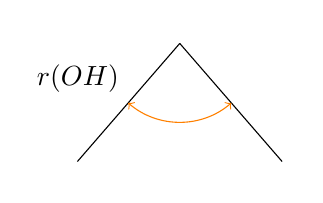
\begin{tikzpicture}
   \Odraw{0,1.5}
   \Hdraw{-1.3,0}
   \Hdraw{1.3,0}
%  \shade[inner color=blue,outer color=red] (0,0) rectangle (4,4);
%  \shadedraw[inner color=blue,outer color=red, draw=black] (0,0) rectangle (4,4);
  \draw(0,1.5) node[circle,minimum size=.4cm] (O) {};
  \draw(-1.3,0) node[circle,minimum size=.3cm,] (H1) {};
  \draw(1.3,0) node[circle,minimum size=.3cm,] (H2) {};
  %\draw(1.3,0) node[circle,minimum size=.2cm,draw,fill=blue] (H2) {};
  %\draw(.65,.8) node[circle,minimum size=.5cm,draw,fill=blue] (O) {};
 % \draw (A.center) -- (B.center);
\begin{pgfonlayer}{background}
 \draw (O.center) -- node[above left] {$r(\te{OH})$}(H1.center);
 \draw (O.center) --  (H2.center);
  \draw pic["$\anghoh$", draw=orange, <->, angle eccentricity=1.2, angle radius=1.cm]
    {angle=H1--O--H2};
\end{pgfonlayer}
 \end{tikzpicture}
\end{equation*}
 \caption{The geometry of $\tip$ water. O is red, H is blue. Each atom coincides with a site with charge $q$ and
  LJ-paramteres $\eps$ and $\si$.}
\label{Fig:Theo:TIP3Geo}
\end{figure} 

When there is no bond formation or breaking to be expected, the framework of
classical mechanics is often also suited to describe a system. That means that
the position of the atomic cores is again a sharply determinable quantity
and motion is governed by forces. All particles move in a classical potential.
We will only treat water molecules as classical particles, so we need a good
%% CHECK: Real source by Jorgensen? Or 1981 source?
classical model of water. We decided on the quite popular $\tip$ potential 
by Jorgensen \etal \cite{Jorgensen1983TIP3P}. The geometry can be
seen in Figure \ref{Fig:Theo:TIP3Geo}. The three sites of the $\tip$ potential
coincide with the atoms forming $\hto$. Each site has a charge $\qal$ with 
\ep{Coulomb interaction}
\begin{equation}
\EC(\ralbe)=\frac{1}{4\pi\eps_0}\frac{\qal\qbe}{\ralbe},
\label{Theo:TIP3EC}
\end{equation}
where $\al,\be$ are the site types and $\ralbe$ is the distance between
the sites $\al$ and $\be$ located at two different water molecules. Sites also
interact by Van-der-Waals forces which are described by a \ep{Lennard-Jones}
(LJ) potential \newcommand\ELJ{\enmat V^{\te{LJ}}_{\al\be}}
\newcommand\salbe{\enmat{\si_{\al\be}}}
\newcommand\ealbe{\enmat{\eps_{\al\be}}}
\begin{equation}
\ELJ(r)=4\ealbe\ed{\rb{\frac{\salbe}{\ralbe}}^{12}-\rb{\frac{\salbe}{\ralbe}}^{6}}.
\label{Theo:TIP3ELJ}
\end{equation}
The original $\tip$ model only had LJ interaction between the oxygen atoms. In
the CHARMM \cite{CHARMM2009} implementation which we use, the H atoms are LJ
sites as well.
Therefore, a $\tip$ water molecule $i$ moves in the potential of all other $\tip$ waters by
\begin{equation}
V_i(\r_i)=\sum_{j\neq i} \sum_{\al,\be} \ed{\EC(\ralbe(\r_i,\r_j)) + \ELJ(\ralbe(\r_i,\r_j))}.
\label{Theo:TIP3Potential}
\end{equation}
The first sum runs over all other water molecules and the second over all
pairs of sites. \eqref{Theo:TIP3Potential} contains only
intermolecular interaction. There would also be the possibility to include intramolecular degrees of freedom with
harmonic potentials for bond and angle stretching. This is not the case for $\tip$,
where all sites are fixed within the molecule, reducing the 9-dimensional coordinate
\mbox{$\r_i=\r_i\rb{\r_{\te O},\r_{\te H1},\r_{\te H2}}$} to a 6-dimensional one, \mbox{$\r_i=\r_i\rb{\r_{\te O},\Om}$}
with the orientational dependence described by $\Om\in\R^3$.

The parameters $\ealbe$, $\salbe$ and $\qal, \qbe$ as well as the geometric parameters
$\r(\te{OH})$ and $\anghoh$ define the $\tip$ potential. They are chosen to reproduce
(macroscopic) thermodynamic properties of a pure water system.
%% CHECK if heats. Wikipedia nennt eine andere Quelle dafür.
The CHARMM $\tip$
potential is fitted to yield good specific heats \cite{MacKerell1998CHARMMTIP3}.  

\subsection{QM/MM}
\label{Sec:Theo:QMMM}

We already motivated using both QM and MM calculations simultaneously due to
the speed of MM and the accuracy of QM results. The simultaneous use
demands some notion of coupling between the two systems. The original
QM/MM coupling scheme proposed by Warshel and Levitt \cite{Warshel1976QMMM}
is nowadays only one among several schemes.
%% CHECK: Dringend checken, ob das irgendwie stimmt.
We chose an approximation
in which the QM part is subject to the external potential defined
by the MM charges and the MM part interacts with the QM atoms by
the LJ potential \eqref{Theo:TIP3ELJ}. That way, the electrostatic
interaction is covered by the QM part while the MM part accounts for
VdW interaction.

\subsection{Energy Minima and Transition States}
\label{Sec:Theo:Minima}
Finding energy minima of the PES for QM or QM/MM systems is basically following
the path defined by the gradient (force)
\newcommand\RM{\enmat{\bo R^M}}
\begin{equation}
\bo F(\RM)=-\nabla V(\RM)
\label{Theo:ForceGradient}
\end{equation}
of the total system's energy $V(\RM)$, where $\RM$ is the vector containing
all atomic coordinates. Again, there is no knowing whether this leads to
a global or a local minimum.

%The gradient of the energy in a quantum mechanical system described by DFT can
%be calculated analytically\cite{VersluisZiegler1988}.

When working on a computer, \eqref{Theo:ForceGradient} must be integrated
in a discretised form. This is best done with step sizes depending on the
value of $\bo F$ and of course one needs tolerances that define convergence.
We used the $\dlfind$ algorithm \cite{Kaestner2009} with the default tolerances
to follow the minimum energy path.

Evaluating the gradient in \eqref{Theo:ForceGradient} is fortunately not
expensive in comparison to a single energy evaluation of the QM part. The gradient of
the MM region can be calculated straighforwardly from \eqref{Theo:TIP3Potential}.
For the QM region, there are schemes to obtain analytical results for the gradient
for a given wave function\cite{VersluisZiegler1988}.
%% CHECK: do they ignore QM/MM?

%% CHECK: Pre-reactive complex?
%\newcommand\ebased[2]{exp(-(\x-#1)^2/#2)} 
\begin{figure}[b!]
%\includegraphics{
% \tikzsetexternalprefix{TikzPics/Theo/}
% \tikzsetnextfilename{Fig.Theo.PES} 
% \begin{equation*}
% \begin{tikzpicture}
%   \draw[->] (-3.7,0) -- (5,0) node[right] {$\xi$};
%   \draw[->] (-3.4,-.3) -- (-3.4,4.5) node[above] {$E$};
%   \draw[domain=-2.4:4.1,smooth,variable=\x,blue] plot ({\x}, {1+3*\ebased{1}{1.5}-1*\ebased{2}{.6}+2*\ebased{4}{3}});%{4*\ebased{2}{3}});
%   \draw[domain=4.1:4.3,smooth,variable=\x,blue] plot ({\x}, {3.0});%{4*\ebased{2}{3}});
%   \draw[dotted] (2.3,-.1) node[below] {$\xi_{\te {MIN}}$} -- (2.3,4.3) ;
%   \draw (1.9,1.87) -- (2.7,1.87) node[right] {$E_{\te {MIN}}$};
%   \draw[dotted] (.9,-.1) node[below] {$\xi_{\te {TS}}$} -- (.9,4.3) ;
%   \draw (.5,3.93) -- (1.3,3.93) node[right] {$E_{\te {TS}}$};
%   \draw[dotted] (-2.4,-.1) node[below] {$\xi_{0}$} -- (-2.4,4.3) ;
%   \draw (-2.6,1.004) node[left] {$E_{0}$} -- (-2,1.004) ;
% \end{tikzpicture} 
% \end{equation*}
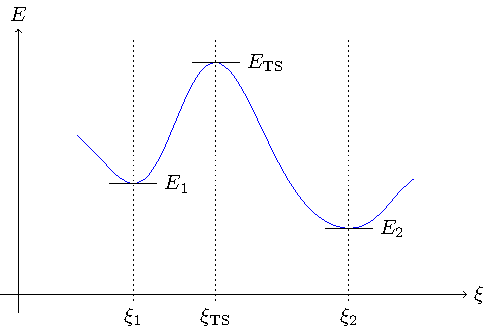
\includegraphics[width=.5\textwidth]{TikzPics/TikzCreation/TheoTS/TheoTS.pdf}
 \caption{A cut of a PES along reaction coordinate $\xi$. The reaction coordinate starts
 at some initial minimum $\xi_1$ with energy $E_1$ and follows a path of minimum
 energy to a neighboring minimum.
 The second minimum with $E_{2}$ is located at $\xi_{2}$. The transition state
 between the two with $E_{\te{TS}}$ is a maximum at $\xi_{\te {TS}}$.}
\label{Fig:Theo:PES}
\end{figure} 

We will also calculate a \ep{transition state} (TS). This
is the state of maximum energy along a \ep{reaction path}, that is a path that
starts at some initial optimum geometry with initial \ep{reaction coordinate}
$\xi_0$ and then follows the direction corresponding to the lowest eigenvalue of the
Hessian matrix to a saddle point (commonly called the transition state) and
after that reaches a new minimum by continuing on its route along the gradient. In Figure
\ref{Fig:Theo:PES}, an example of such a path between reaction coordinates
$\xi_1$ and $\xi_{2}$ is plotted.

%% CHECK: ZITAT. Außerdem Theorie checken!
In this work, we obtain transition states with the \ep{dimer method}
\cite{HenkelmanJonsson1999}. It uses two images of the system with a slight offset, then
rotates them to find the eigenvector to the minimum eigenvalue of the Hessian
matrix \eqref{Theo:Hessian}. It follows these minimum eigenvalue directions by an
iterative scheme until a saddle point is reached. This is the transition state.

Transition states are important for calculating activation energies as well as
reaction and tunneling rates. The former govern reaction rates while the latter
are also interesting for the analysis of molecule formation on ice surfaces since at
temperatures as low as in the interstellar medium, tunneling has a significant
contribution to the dynamics of these systems.

\subsection{Technical Details}

%% CHECK: Sollte nwchem noch rein?
Before proceeding to actual calculations, we want to mention the programs and tools 
used for these. As we already mentioned, the optimisations are carried out with
$\dlfind$ \cite{Kaestner2009}, as are the dimer method and the calculation of 
Hessian matrices. DFT calculations are performed with TURBOMOLE\cite{TURBOMOLE}.
Force field calculations are performed by CHARMM \cite{CHARMM2009}. These programs were interfaced
via ChemShell \cite{chemshell,MetzKaestnerSokolEtAl2013}, which also provided
the QM/MM coupling.

For the post-HF calculations in the benchmark, we used the MOLPRO \cite{MOLPRO_brief}
package.

All molecular visualisations are created with VMD \cite{HUMP96}.

%% CHECK: Mehr Details zum JUSTUS?
The calculations were performed on the bwForCluster JUSTUS of the German federal country
of Baden-Württemberg. Shared memory parallel calculations with up to 16 CPUs
were performed. The main limit was the maximal computation time of six days.


%\subsection{The Fletcher Surface}
%\label{Sec:Theo:Fletcher}

\section{Benchmarking}
\newcommand\htohto{\mbox{\enmat{\hto-\hto}}}
\newcommand\htoo{\mbox{\enmat{\hto-\hspace{.2pt} ^3\te{O}}}}
\newcommand\htoh{\mbox{\enmat{\hto-\te H}}}
\label{Sec:Bench}

In the previous section, we introduced the basic notions of the theoretical
structure underlying our computations. We mentioned already that the choice
of DFT functionals and basis sets is of great importance to the accuracy of our calculations. Unfortunately, not much can be said a priori about
which functional combined with which basis set should be used to describe a certain system.
There are recommendations as some functionals were fitted to best represent a certain
group of elements or reactions, but in order to determine the reliability of
future results, there is no way around literature research and own benchmark
tests.

We already
discussed the functionals we want to test in Section \ref{Sec:Theo:Functionals}, and we
have reason to hope that at least the \pbez, $\pw\dt$ and $\bns\dt$ functionals will be sufficiently
accurate to describe water-water interaction, as they are recommended by Anacker and Friedrichs \cite{Anacker2014}.
The basis sets we want to compare alongside the functionals are those mentioned
in Section \ref{Sec:Theo:Basis}.

In order to perform a benchmark study we use the three interaction energies of
the $\htoh$, $\htohto$ and $\htoo$ systems.
The reference calculations were in all cases performed with the MOLPRO \cite{MOLPRO_brief} package
at the $\ccsdtf$ \cite{KniziaAdlerWerner2009} level of theory with the
$\vtz$\cite{YousafPeterson2008} basis set, for which we found energy minima.
%minima\footnote{In the $\htoo$ case, a first minimum was calculated at the
%$\mrcif/\vtz$ \cite{ShiozakiKniziaWerner2011} level of theory, where it was
%found that the wavefunction can be well described by a single-reference method.
%From there, the $\ccsdtf$ minimisation was carried out.}.
For $\htoo$, the $\ccsdtf$ calculations were preceded by \ep{multi-reference} 
calculation at the $\mrcif/\vtz$\cite{ShiozakiKniziaWerner2011} level of theory
including Davidson correction\cite{LanghoffDavidson1974} to find an optimum
geometry, which turned out to be suitable for single-reference treatment.

At each optimum geometry, an additional calculation was carried out to find a CP
corrected energy. For $\htoh$ and $\htohto$, this calculations was also at the $\ccsdtf/\vtz$ level
of theory, while for the $\htoo$ interaction again an $\mrcif/\vtz$ calculation was
required due to the necessity of a multireference treatment of the case where the
$^3\te O$ radical is set as a dummy atom. In all cases, the $\vtz$ basis set is 
large enough to require only small CP corrections of $0.05 - 0.18 \ \kmo$. 
%We used these minima as initial geometries for two different
%types of reference calculations:
%% CHECK: Sollte man Benchmark i. überhaupt erwähnen? Meine Schlussfolgerung: Nein.
%\begin{enumerate}[i.]
%  \item Energy reference: No minimisation was performed. Instead, the $\ccsdtf/\vtz$ geometries
%    were used and the energy values are compared.
%  \item Geometry reference: The initial geometries were further optimized to arrive at a minimum
%    geometry and energy corresponding to the DFT method.
%\end{enumerate}

We performed energy minimisations at the DFT level of theory with different basis sets. The initial
geometry was always the reference geometry provided by the $\ccsdtf$ calculation. The results can be compared
to the coupled-cluster data with respect to optimum geometry and energy deviations. We will discuss
these for the three test systems separately.

The deviation in interaction energy is calculated by 
\newcommand\ecc{\enmat{\eint_{\te {CC}}}}
\begin{equation}
\Dl\eint=\eint\dft-\ecc.
\label{Bench:RefEnergy}
\end{equation}
$\eint\dft$ stands for the interaction energy \eqref{Theo:InteractionEnergy} of
the system computed with a certain DFT functional and basis set, and $\ecc$ is
the CP corrected interaction energy with $\ccsdtf/\vtz$.

The deviation of optimum geometry \mbox{$\bo R^M\dft=(\r^1\dft,\ldots,\r^M\dft)$} from the reference optimum geometry 
\mbox{$\bo R^M\cc=(\r^1\cc,\ldots,\r^M\cc)$} can be quantified by the \ep{root mean square deviation} (RMSD). It
is given by
\newcommand{\DRMSD}{\Dl_{\te{RMSD}}}
\begin{equation}
\Dl_{\te{RMSD}}(\bo R^M\dft;\bo R^M\cc)=\sqrt{\frac 1 M \sum_{k=1}^M \abs{\r^k\dft-\r^k\cc}^2}.
\label{Bench:RMSD}
\end{equation}
We will give $\DRMSD$ in $\Ang$.   

%% CHECK: Source?
Note that, obviously, the coupled cluster results are approximations just as the DFT results, however
there is good reason to assume that they are more accurate. For the following comparisons, we will
therefore consider the coupled cluster results as if they were the correct values for this
interaction.

%% CHECK: Speedup-table?
Another remark before starting the discussion is the accuracy with which
numerical integration was carried out. In the \mbox{TURBOMOLE} code, we used an
m4 integration grid with keyword ``\$scfconv 8''. The results have been compared
to the more accurate m5 grid and ``\$scfconv 9'', which did not result in
a change in energy.
Therefore, we recommend the less accurate technique due to it being
computationally faster while being very close to the more accurate alternative.

\subsection{$\htoh$ Interaction}

\tikzsetexternalprefix{TikzPics/Benchmark/}
\tikzsetnextfilename{Fig.Bench.H2O+H.NoD3}
\pgfplotsset{xtick style={draw=none}}
\begin{figure}[b!]
\centering
\begin{tikzpicture}
\begin{axis}[
    height=8cm,
    width=.48*\textwidth,
    ybar,
    xmin=.5,
    xmax=9.5,
    ymin=-.7,
    ybar=0pt,
    axis x line*=bottom,
    enlarge x limits=0.015,
    enlarge y limits=0.15,
    legend style={legend pos=south west,font=\small,legend columns=1},
    ylabel={interaction energy deviation $\Delta \eint$ / kJ/mol},
    xticklabels={\btlyp,\bns,\bhlyp,\blyp,\bp,\pbe,\pbez,\tpssh,\pw},
    xtick=data,
    grid=minor,
    xticklabel style={rotate=90},
    bar width = .008*\textwidth,
    minor xtick={1.5,...,8.5},
    yticklabel pos=left,
    grid style={dotted,gray},
    ymajorgrids=true,
    ]
\addplot[green!20!black,fill=green!80!white] coordinates {(1,-.17957936646) (2,.36521188354) (3,-.07314159646) (4,-.13145395146) (5,-.02562004646) (6,-.61493977646) (7,-.15329811146) (8,.02935792354) (9,-.32041118646) };
\addplot[blue!20!black,fill=blue!80!white] coordinates {(1,-.09364675146) (2,.38435177854) (3,-.01343772646) (4,-.05111365146) (5,.03597418354) (6,-.44399347146) (7,-.07471689646) (8,.01756942854) (9,-.20565058146) };
\addplot[red!20!black,fill=red!80!white] coordinates {(1,.19741617854) (2,.35121796854) (3,.18210951354) (4,.39813565354) (5,.23267664354) (6,-.19932312646) (7,.09974757854) (8,.23782262354) (9,.03978115854) };
\addplot[yellow!20!black,fill=yellow!80!white] coordinates {(1,.06989564354) (2,.35788673854) (3,.11838862854) (4,.18512883854) (5,.12862807854) (6,-.28819630146) (7,.04897040854) (8,.12219560354) (9,-.03386411646) };

%\addplot[green!20!black,fill=green!80!white] coordinates {(1,-1.38867462646) (2,.35885817354) (3,-.79392011146) (4,-1.88993508646) (5,-2.70903857646) (6,-1.89731274146) (7,-.85296760646) (8,-7.27761861646) (9,-5.38880766146) (10,-.34732256146) };
%\addplot[blue!20!black,fill=blue!80!white] coordinates {(1,-.45181746146) (2,.40364920354) (3,-.14531659146) (4,-.86748662146) (5,-3.06760311146) (6,-.56095949646) (7,-.09096874146) (8,-8.76869257646) (9,-6.56655445146) (10,-.21066528646) };
%\addplot[red!20!black,fill=red!80!white] coordinates {(1,.13821115354) (2,.35153302854) (3,.15884758354) (4,.31267562854) (5,-2.18406985146) (6,-.85294135146) (7,-.24025467146) (8,-7.37633741646) (9,-5.39749806646) (10,-.02593510646) };
%\addplot[yellow!20!black,fill=yellow!80!white] coordinates {(1,-.18921495146) (2,.38823751854) (3,.03639426354) (4,-.31846831646) (5,-2.69564852646) (6,-.73300851146) (7,.01846209854) (8,-8.12079794146) (9,-6.01869136646) (10,-.09808384646) };
\legend{def2-SVPD,def2-TZVP,def2-TZVPD,def2-QZVP}
\end{axis}
\end{tikzpicture}
%\captionsetup{format=hang}
%\setcapmargin[4cm]{1cm}
\caption{The $\htoh$ benchmark results for different basis sets without dispersion correction.
Energies are plotted as differences to the reference energy from $\ccsdtf/\vtz$ calculations,
see \eqref{Bench:RefEnergy}.}
\label{Fig:Bench:H2O+H:NoD3}
\end{figure}

\textbf{Reference energy.} For $\htoh$, we found \mbox{$\ecc=-0.40\ \kmo$}, so
we have an only weakly bonded system. The CP correction contributes $+0.05\ \kmo$ to
the energy.

\textbf{Basis set.} For basis set comparison, we focus on Figure
\ref{Fig:Bench:H2O+H:NoD3}. The basis sets grouped from most attractive to
least attractive interaction energies are $\svpd$, $\tzvp$, $\qzvp$ and
$\tzvpd$.
For most functionals, $\tzvp$ is the most accurate functional.

Figure \ref{Fig:Bench:H2O+H:NoD3} does not contain our results for the def2-SVP basis
set since they are much worse than all other results -- up to $-20\ \kmo$ and
usually more than $-5\ \kmo$ of deviation. However, the addition of diffuse
functions effects quite a remarkable improvement to the def2-SVP results, such
that def2-SVPD calculations are well comparable to results obtained by basis
sets of more than double-$\zeta$ order.

It is also noteworthy that def2-QZVP does not seem to offer a clear advantage over the
other three basis sets in Figure \ref{Fig:Bench:H2O+H:NoD3}. It tends to yield
similar accuracy as def2-TZVPD, while usually being inferior to def2-TZVP for
most functionals. def2-QZVP takes on average 1.44 times as long to complete an
energy and gradient calculation iteration as def2-TZVPD, which in turn takes
on average only 1.02 times as long as an energy and gradient calculation with
$\tzvp$.
%From a first glance
%at the ``better'' functionals in this case, one could therefore consider
%the def2-TZVP and def2-TZVPD basis sets as good compromises between
%accuracy and computational cost.

\tikzsetexternalprefix{TikzPics/Benchmark/}
\tikzsetnextfilename{Fig.Bench.H2O+H.D3}
\begin{figure}[b!]
\centering
\begin{tikzpicture}
\begin{axis}[
    height=8cm,
    width=.48*\textwidth,
    ybar,
    xmin=.5,
    xmax=9.5,
    ybar=0pt,
    axis x line*=bottom,
    enlarge x limits=0.015,
    enlarge y limits=0.15,
    legend style={legend pos=south west,font=\small,legend columns=1},
    ylabel={interaction energy deviation $\Delta \eint$ / kJ/mol},
    xticklabels={\btlyp\dt,\bns\dt,\bhlyp\dt,\blyp\dt,\bp\dt,\pbe\dt,\pbez\dt,\tpssh\dt,\pw\dt},
    xtick=data,
    grid=minor,
    xticklabel style={rotate=90},
    bar width = .008*\textwidth,
    minor xtick={1.5,...,8.5},
    yticklabel pos=left,
    grid style={dotted,gray},
    ymajorgrids=true,
    ]
 \addplot[green!20!black,fill=green!80!white] coordinates {(1,-2.39332220146) (2,.33675146354) (3,-.76816395646) (4,-2.85861331146) (5,-5.18753683146) (6,-1.37496951646) (7,-.86554375146) (8,-.85577689146) (9,-.66041343646) };
\addplot[blue!20!black,fill=blue!80!white] coordinates {(1,-2.17766363146) (2,.32630197354) (3,-1.22998940646) (4,-4.40490153646) (5,-6.08159834646) (6,-1.20436452646) (7,-.78775018646) (8,-.86803797646) (9,-.54581036146) };
\addplot[red!20!black,fill=red!80!white] coordinates {(1,-2.12935443146) (2,.32170734854) (3,-.51228272646) (4,-3.21961956146) (5,-5.29358077646) (6,-.95937912146) (7,-.61265559146) (8,-.64757474146) (9,-.29990603146) };
\addplot[yellow!20!black,fill=yellow!80!white] coordinates {(1,-1.96625837146) (2,.35990837354) (3,-.57660747646) (4,-3.79917243146) (5,-5.74679458646) (6,-1.04856735646) (7,-.66372156646) (8,-.76354307646) (9,-.37368258146) };

%\addplot[green!20!black,fill=green!80!white] coordinates {(1,-1.97799435646) (2,.32338766854) (3,-1.22313685146) (4,-3.62034962646) (5,-3.92406746646) (6,-2.72187727146) (7,-1.68002636146) (8,-9.09123525146) (9,-7.27662092646) (10,-.69927083646) };
%\addplot[blue!20!black,fill=blue!80!white] coordinates {(1,-2.78000584146) (2,.32165483854) (3,-1.43427956146) (4,-4.40482277146) (5,-6.08157209146) (6,-1.46258245146) (7,-.92795188646) (8,-10.45730915646) (9,-8.34535695646) (10,-.56957113646) };
%\addplot[red!20!black,fill=red!80!white] coordinates {(1,-1.53727792646) (2,.32107722854) (3,-1.13329224146) (4,-3.21954079646) (5,-5.29355452146) (6,-1.65534666146) (7,-1.02512164146) (8,-9.05471454646) (9,-7.20799035646) (10,-.30591842646) };
%\addplot[yellow!20!black,fill=yellow!80!white] coordinates {(1,-2.45502145146) (2,.35329211354) (3,-1.26023516646) (4,-3.79922494146) (5,-5.74687335146) (6,-1.38919972646) (7,-1.00191222146) (8,-9.77473166646) (9,-7.77722501146) (10,-.39245490646) };
\legend{def2-SVPD,def2-TZVP,def2-TZVPD,def2-QZVP}
\end{axis}
\end{tikzpicture}
\caption{The $\htoh$ benchmark results for different basis sets and
functionals including dispersion correction.
Energies are plotted as differences to the reference energy from $\ccsdtf/\vtz$ calculations,
see \eqref{Bench:RefEnergy}.}
\label{Fig:Bench:H2O+H:D3}
\end{figure}

\textbf{Functionals and dispersion correction.} Again, we focus on the data in
Figure \ref{Fig:Bench:H2O+H:NoD3}. Comparing functionals with the $\tzvp$ basis set,
the most accurate results are obtained by $\bhlyp$, $\tpssh$ and $\bp$, mediocre
results are obtained by $\blyp$, $\pbez$ and $\btlyp$. The $\pw$ functional
has its best result at the $\tzvpd$ basis set.

The results here seem to be very accurate in
absolute deviation, while relative deviations are often greater than 50\%.
Therefore, we can generally say that the description of $\htoh$ seems to be
tricky with the functionals and basis sets we used in this test. 
%% CHECK: Accuracy ccsd(t)?
%Still, the deviations are within the error bonds of a $\ccsdtf$ calculation,
%so it is hard to favour a functional of the given choice.
A few functionals need special remarks, but rather for their deficiencies. The
first one are the $\tpss$ and $\tpss\dt$ functionals. They predict much too
attractive energies for this benchmark, beyond $-7\ \kmo$ and $-9\ \kmo$,
respectively.
%% CHECK: Vergleich, ob das jedesmal etwa derselbe Abstand ist (basis- und dispersionsabhängig).
They predict
a wrong optimum geometry, where the H radical is at a distance of around $2.20\ \Ang$
from the O atom in the water molecule, which is much less than the reference
value of $3.34\ \Ang$. 

The opposite problem happens for $\bns$ and $\bns\dt$ optimisations. Here, the attraction is
considered close to being repulsive, with interaction energy values around
\mbox{$\eint_{\bns}\approx -0.03\ \kmo$}. While the resulting deviation of around
$0.37\ \kmo$ does not look too dramatic in Figures \ref{Fig:Bench:H2O+H:NoD3} and
especially Figure \ref{Fig:Bench:H2O+H:D3}, it is a qualitative mistake. The
separation between radical H and water O is around $5.80\ \Ang$, which is close to describing two isolated
systems.

The inclusion of the D3 dispersion correction is
not beneficial to the interaction energy values of $\htoh$, which can be seen
by comparing Figure \ref{Fig:Bench:H2O+H:NoD3} to Figure
\ref{Fig:Bench:H2O+H:D3}. Indeed, while most functionals without dispersion
corrections have errors of between $-0.2$ and $+0.2\ \kmo$ for at least one
basis set, the D3 corrected versions deviate stronger than $-5\ \kmo$.
The contribution of dispersion in $\htoh$ is therefore strongly overestimated
by the D3 correction. The best results for dispersion corrected functionals are
obtained by $\pw\dt/\tzvpd$ with a deviation of $-0.30\ \kmo$.


\textbf{Optimum geometry.} Comparing RMSD data of different functionals yields similar results as the energy comparison.
Functionals without the D3 correction
predict very accurate geometries with \mbox{$\DRMSD < 0.01\ \Ang$} for all but
$\tpss$ and $\bns$.
Despite worse energy results, many D3 corrected versions still find accurate optimum geometries.
Exceptions are $\btlyp\dt$, $\blyp\dt$, $\bp\dt$, which find optima similar
to the already mentioned $\tpss$ optimum, with the H radical too close to the water O.
%% CHECK: Im Original stand bhlyo, aber das glaub ich nicht. Bhlyp-d3
% vermutlich.
The $\bhlyp\dt$ functional generally yields good geometries, only for the
$\tzvp$ basis set it also predicts the H radical too close to the water O.

Concerning the change of optimum geometry with respect to the choice of basis
set, most basis sets lead to the same optimum geometry for nearly all
functionals. Again, the \mbox{$\svp$} basis set and the $\tzvpp$ basis set often
predict wrong, i.e. too attractive, geometries. 

% Let us now look at the different functionals. The $\bns$ functional
% seems to offer a very good approximation to $\ecc$  with and without dispersion
% correction. This is unfortunately not due to the functional's accuracy but instead
% it appears that the functional
% considers the $\htoh$ interaction to be repulsive in the region where most functionals
% find an energy minimum, so it finds a less attractive optimum geometry at
% a much larger distance between the water oxygen and the hydrogen atom.
% A more satisfactory result is produced with the $\pw$ functional. The energies 
% are very accurate both for $\pw$ and $\pw\dt$ and they do not vary strongly with basis set size.
% They are most accurate for the def2-TZVPD basis set with a deviation
% of only $\Dl\eint=-0.025 \kmo$ (no D3 correction) and $\Dl\eint=-0.255 \kmo$ (D3 corrected).
% %The def2-TZVPD basis set is computationally much
% %faster than the def2-QZVP basis set (which takes roughly 1.5 times
% %the computation time of the smaller basis set). 
% For basis sets
% larger than def2-SVPD the $\btlyp$, $\bhlyp$ and $\pbez$ functionals yield very good
% results as well, although the dispersion corrected version are significantly less accurate.
% The $\tpss$ and $\tpssh$ functionals should not be used to describe this interaction,
% while $\btlyp$ and $\blyp$ can be considered quite good -- not as good as
% $\pw$, $\bhlyp$ or $\pbez$ but much better than $\tpss$ and $\tpssh$ -- while they become
% worse with additional dispersion.
% 
% So from the $\htoh$ data, one can already conclude that the $\tpss$ and $\tpssh$
% functionals should not be expected to yield good energy values for hydrogen adsorption,
% which may however still occur due to error cancellation. The $\bns$ functional
% is probably also not fit to describe such a system accurately. Furthermore, the def2-SVP basis
% set is not fit to describe $\htoh$ interaction. Since they are sufficiently accurate
% while not too expensive, we will especially evaluate the def2-TZVP basis set family
% for $\htohto$ interaction.
%% CHECK: Table mit Computation times?
%% CHECK: RMSD table?

\tikzsetexternalprefix{TikzPics/Benchmark/}
\tikzsetnextfilename{Fig.Bench.H2O+H2O.BasisCompare}
\begin{figure}[h]
\centering
\begin{tikzpicture}
\begin{axis}[
    height=8cm,
    width=.493*\textwidth,
    ybar,
    xmin=.5,
    xmax=3.5,
    ybar=0pt,
    ymax=2.5,
    axis x line*=bottom,
    enlarge x limits=0.015,
    enlarge y limits=0.15,
    %legend pos=south east,
    legend style={legend pos=north west,font=\small,legend columns=3},
    ylabel={interaction energy deviation $\Delta \eint$ / kJ/mol},
    xticklabels={\bhlyp,\pbez,\pw\dt},
    xtick=data,
    grid=minor,
    %xticklabel style={rotate=90},
    bar width = .010*\textwidth,
    minor xtick={1.5,2.5},
    minor ytick={-4,...,2},
    yticklabel pos=left,
    grid style={dotted,gray},
    ymajorgrids=true,
    ]


\addplot[green!20!black,fill=green!80!white] coordinates {(1,-1.9936404330) (2,-2.2264697730) (3,-2.3673015930) };
\addplot[blue!20!black,fill=blue!80!white] coordinates {(1,-3.4503203430) (2,-3.9391359330) (3,-4.0300832530) };
\addplot[brown!20!black,fill=brown!80!white] coordinates {(1,-1.9095719230)
(2,-2.4086269630) (3,-2.5282447430) }; \addplot[red!20!black,fill=red!80!white] coordinates {(1,-.1324234830) (2,-.2683193630) (3,-.3517577530) };
\addplot[orange!20!black,fill=orange!80!white] coordinates {(1,.2438106670) (2,.1062344670) (3,.0347158470) };
\addplot[yellow!20!black,fill=yellow!80!white] coordinates {(1,-.5243581230) (2,-.9162402530) (3,-.9979458130) };
\addplot[purple!20!black,fill=purple!80!white] coordinates {(1,.2676502070) (2,.1384230970) (3,.0622835970) };
\legend{def2-SVPD,def2-TZVP,def2-TZVPP,def2-TZVPD,def2-TZVPPD,def2-QZVP,def2-QZVPD}

\end{axis}
\end{tikzpicture}
\caption{The $\htohto$ benchmark results for $\bhlyp$, $\pbez$ and $\pw\dt$ and all
basis sets used in the study (excluding \mbox{def2-SVP}). Energies are plotted as differences
to the reference energy from $\ccsdtf/\vtz$ calculations, see \eqref{Bench:RefEnergy}.}
\label{Fig:Bench:H2O+H2O:BasisCompare}
\end{figure}


\subsection{$\htohto$ Interaction}

\textbf{Reference energy.} The reference energy for the $\htohto$ dimer is at
\mbox{$\ecc=-20.80\ \kmo$}, where the CP correction contributes $+0.18\ \kmo$.

\textbf{Basis sets.} We use three promising functionals to investigate the difference
between basis sets in Figure \ref{Fig:Bench:H2O+H2O:BasisCompare}. Again, the
def2-SVP basis set is not considered, since it yields errors between $-12\ \kmo$ and $-15\ \kmo$ for all three
functionals. The figure shows that while increasing the $\zeta$-order of the basis set
improves the results, inclusion of additional diffuse functions seems to
be even more beneficial. The basis set def2-SVPD is more accurate than def2-TZVP and
def2-TZVPD is more accurate than def2-QZVP.
%% CHECK! Does that make sense? Citation?
This may well be due to reduction of the BSSE, which depends on the ability
of basis sets to describe electrons far from the core.
The inclusion of polarisation functions as in def2-TZVPP also
affects the results positively, however not to the extent of additional
diffuse functions. The def2-TZVPPD basis set is again an improvement
to the def2-TZVPP basis set, it is also slightly more accurate than the
def2-TZVPD basis set. Indeed, for all three functionals the def2-TZVPPD and
def2-QZVPD results are strikingly close to one another, which could
be an indication that the basis set truncation error is low and that
the intrinsic quality of the methods is reached. In that case, the
three functionals analysed in Figure \ref{Fig:Bench:H2O+H2O:BasisCompare} are
all capable of yielding excellent approximations to our coupled-cluster data,
and the results at the def2-TZVPD basis set are already close to the
methods' intrinstic error.  

Concerning speedup, here $\tzvpd$ takes on average $1.16$ times as long as
$\tzvp$ for a single energy and gradient calculation, and $\qzvp$ takes $2.18$
times as long as $\tzvpd$.

The results so far speak in favour of the def2-TZVPD basis set. Due 
to the size of the quantum mechanical part of the QM/MM system we will later consider,
it is computationally too expensive to use $\tzvpd$ for the whole
QM part. We will therefore use a hybrid basis set with the more important atoms
described by the def2-TZVPD basis set and the less important ones by the
def2-TZVP basis set. We will describe this further subdivision of the QM domain
in more detail in Section \ref{Sec:Ads:Model}.

We should therefore determine functionals that are both good for def2-TZVP and def2-TZVPD,
while their accuracy for def2-TZVPD is more important since the adsorption site will
be closer to the def2-TZVPD atoms. 

\textbf{Functionals and dispersion correction.} In Figure
\ref{Fig:Bench:H2O+H2O:TZVPCompare}, we take a look at the differences between dispersion corrected and not dispersion
corrected results in the def2-TZVP and def2-TZVPD basis sets. The stronger
attraction between the two $\hto$ molecules prevents errors as for the
$\bns$ functional in the previous section, so all functionals expect attractive
interaction. Inclusion of the D3 dispersion correction again predicts
stronger attraction, while the additional diffuse functions of the def2-TZVPD
basis set weaken the attraction. These effects can combine to yield good
results, for example for $\bns\dt$ or $\pw\dt$.
%the high accuracy of $\pw\dt$ with the def2-TZVPD basis set. 

%Dispersion corrections , this may well be due to the more important role of dispersion for this interaction. 
The inaccuracy of some functionals may be due to the bad treatment of
dispersion in DFT. But inclusion of the D3 correction does not resolve the issue for cases
where the interaction is already too attractive. This
is most striking for the def2-TZVP basis set, which predicts too attractive
interaction for all functionals but $\bns$. Generally, every functional has its
most accurate results -- either in the standard or the dispersion corrected version --
at the def2-TZVPD basis set. Excellent
results at the $\tzvpd$ level are obtained by $\bhlyp$, $\pbez$ and $\pw\dt$,
but they are all not too accurate in the $\tzvp$ basis set.  

Good compromises between the $\tzvp$ and $\tzvpd$ basis sets
are therefore given by $\btlyp$, $\tpss$, $\tpssh$ and $\pw$, which all give
mediocre results in both basis sets. $\bhlyp$, $\pbez$ and $\pw\dt$ are highly
accurate for def2-TZVPD but not very good with def2-TZVP. $\bns\dt$ is somewhat
between those functionals, being less accurate for def2-TZVPD but still better
for def2-TZVP than e.g. $\pbez$. All other functionals are not accurate enough
for def2-TZVP or def2-TZVPD.

% Another
% result that reappears is the good accuracy of the $\bhlyp$ and $\pbez$ functional
% without dispersion correction in the def2-TZVPD basis set, however both are
% not too accurate with def2-TZVP. Another very good functional is 
% the already mentioned $\pw\dt$, which is also only strikingly good with
% def2-TZVPD. 

\tikzsetexternalprefix{TikzPics/Benchmark/}
\tikzsetnextfilename{Fig.Bench.H2O+H2O.TZVPCompare}
\begin{figure}[h]
\centering
\begin{tikzpicture}
\begin{axis}[
    height=8cm,
    width=.48*\textwidth,
    ybar,
    xmin=.5,
    xmax=10.5,
    ybar=0pt,
    axis x line*=bottom,
    enlarge x limits=0.015,
    enlarge y limits=0.15,
    legend style={legend pos=north east,font=\small,legend columns=2},
    ylabel={interaction energy deviation $\Delta \eint$ / kJ/mol},
    xticklabels={\btlyp,\bns,\bhlyp,\blyp,\bp,\pbe,\pbez,\tpss,\tpssh,\pw},
    xtick=data,
    grid=minor,
    xticklabel style={rotate=90},
    bar width = .008*\textwidth,
    minor xtick={1.5,...,9.5},
    yticklabel pos=left,
    grid style={dotted,gray},
    ymajorgrids=true,
    ]
\addplot[blue!20!black,fill=blue!80!white] coordinates {(1,-2.4712713930) (2,1.8105515370) (3,-3.4503203430) (4,-1.5251462130) (5,-1.4308382530) (6,-5.0817010230) (7,-3.9391359330) (8,-2.3940816930) (9,-2.2228465830) (10,-2.6678163230) };
\addplot[red!20!black,fill=red!80!white] coordinates {(1,1.4702867370) (2,5.7188708370) (3,-.1324234830) (4,3.0175463970) (5,2.6200456970) (6,-.7830223830) (7,-.2683193630) (8,1.5256322770) (9,1.5457961170) (10,1.0097740370) };
\addplot[blue!20!black,pattern color=blue!80!white,pattern = horizontal lines] coordinates {(1,-5.5127031030) (2,-3.4044266030) (3,-5.8857341430) (4,-5.2560342230) (5,-4.9150342830) (6,-6.9246970030) (7,-5.8901449830) (8,-4.9479580530) (9,-4.7306191630) (10,-4.0300832530) };
\addplot[red!20!black,pattern color=red!80!white,pattern = horizontal lines] coordinates {(1,-1.5693596330) (2,.6348001270) (3,-2.5674172030) (4,-.7562947930) (5,-.8699789430) (6,-2.5687824630) (7,-2.2220064230) (8,-.9511594030) (9,-.9633417230) (10,-.3517577530) };
%\addplot[blue!20!black,fill=blue!80!white] coordinates {(1,-2.2911688300) (2,1.8945608000) (3,-3.3056620300) (4,-1.3177384500) (5,-1.2830293400) (6,-4.9496451100) (7,-3.7824003200) (8,-2.2352456800) (9,-2.0561340700) (10,-2.4866635600) };
%\addplot[red!20!black,fill=red!80!white] coordinates {(1,1.6138948500) (2,5.9163017000) (3,.0413778800) (4,3.1551158600) (5,2.9033304100) (6,-.6073831700) (7,-.1202479000) (8,1.6705531400) (9,1.6996436800) (10,1.2347726500) };
%\addplot[blue!20!black,pattern color=blue!80!white,pattern = horizontal lines] coordinates {(1,-5.3662069400) (2,-3.1298060400) (3,-5.7434387800) (4,-5.0291977600) (5,-4.7869166200) (6,-6.8055060400) (7,-5.7431237200) (8,-4.8009367900) (9,-4.5759839500) (10,-3.8439420400) };
%\addplot[red!20!black,pattern color=red!80!white,pattern = horizontal lines] coordinates {(1,-1.4527941700) (2,.9033820400) (3,-2.3888899400) (4,-.5200065300) (5,-.7710043300) (6,-2.4600935000) (7,-2.0844369600) (8,-.8217289900) (9,-.8236718600) (10,-.1117937900) };
\legend{def2-TZVP,def2-TZVPD,def2-TZVP+D3,def2-TZVPD+D3}
\end{axis}
\end{tikzpicture}
\caption{The $\htohto$ benchmark results for the def2-TZVP and def2-TZVPD basis sets.
The results with dashed bars include dispersion corrections. Energies are plotted as differences
to the reference energy from $\ccsdtf/\vtz$ calculations, see \eqref{Bench:RefEnergy}.}
\label{Fig:Bench:H2O+H2O:TZVPCompare}
\end{figure}

%% CHECK: Sollte das hier kommen? Sollen wir nicht später darauf zurückkommen oder es früher
% erwähnen?
\textbf{Optimum geometry.} For $\htohto$, the RMSD values are 
unproblematic for any basis set beyond $\svp$ (where an entirely wrong geometry is predicted). The worst RMSD is
reached by $\bns\dt/\tzvpd$, it is of \mbox{$0.076\ \Ang$}, which is just a
slight displacement of H atoms. Especially $\btlyp$ and $\pw$ both with and
without dispersion corrections predict RMSDs of less than $0.008\ \Ang$ to the
reference geometry, $\bhlyp$ is roughly at $0.010\ \Ang$ and the rest is
between $0.02$ and $0.05\ \Ang$. Therefore, $\htohto$ interaction geometries
are well described by any functional in a basis set bigger than $\svp$.

% With these hybrid basis set considerations, we can therefore nominate seven functionals
% that may describe water-water interaction in our context sufficiently accurate. If we exclude
% those that have proven very inaccurate for $\htoh$ interaction in these basis sets, we are
% left with only five, $\btlyp$, $\bhlyp$, $\pbez$, $\tpssh$ and $\pw\dt$. We might be able
% to narrow this selection down by considering the third benchmark. 

\subsection{$\htoo$ Interaction}

\textbf{Reference energy.} It already became clear at the beginning of this
section that the $\htoo$ interaction is more tricky for post-HF methods because
some geometries in the optimisation process are not well described by a single
Slater determinant. At the optimum geometry, a single-reference approach is
fortunately possible, so our results for this benchmark have the full
credibility of the $\ccsdtf$ method. Only the CP correction is taken from an
$\mrcif$ calculation, but it is as small as \mbox{$0.10\ \kmo$} and therefore
the error here is unlikely to deteriorate our results. The CP corrected
interaction energy is \mbox{$\ecc=-6.72\ \kmo$}.


\tikzsetexternalprefix{TikzPics/Benchmark/}
\tikzsetnextfilename{Fig.Bench.H2O+O.FuncCompare}
\begin{figure}[h]
\centering
 \begin{tikzpicture}

\begin{axis}[
    height=8cm,
    width=.48*\textwidth,
    ybar,
    xmin=.5,
    xmax=6.5,
    ybar=0pt,
    axis x line*=bottom,
    enlarge x limits=0.015,
    enlarge y limits=0.15,
    legend style={legend pos=south west,font=\small,legend columns=2},
    ylabel={interaction energy deviation $\Delta \eint$ / kJ/mol},
    xticklabels={\btlyp,\bhlyp,\pbez,\tpssh,\pw,\pw\dt},
    xtick=data,
    grid=minor,
    xticklabel style={rotate=90},
    bar width = .008*\textwidth,
    minor xtick={1.5,...,5.5},
    yticklabel pos=left,
    grid style={dotted,gray},
    ymajorgrids=true,
    ]
\addplot[green!20!black,fill=green!80!white] coordinates {(1,-.3260083350) (2,-.8335962500) (3,-1.4244387700) (4,-.4892356700) (5,-1.0877183950) (6,-2.0006572550) };
\addplot[blue!20!black,fill=blue!80!white] coordinates {(1,-.1081968550) (2,-.2511553300) (3,-.9848250500) (4,-.0743016500) (5,-.5862478950) (6,-1.5014446850) };
\addplot[red!20!black,fill=red!80!white] coordinates {(1,.4817004850) (2,.0664251500) (3,-.5893722400) (4,.5068527750) (5,-.0768746400) (6,-.9915725850) };
\addplot[orange!20!black,fill=orange!80!white] coordinates {(1,.5734354550) (2,.1101397250) (3,-.4387210500) (4,.5473904950) (5,-.0140726800) (6,-.9310548100) };
\addplot[yellow!20!black,fill=yellow!80!white] coordinates {(1,.4925700550) (2,.1261815300) (3,-.4793375350) (4,.3330971850) (5,-.0581285700) (6,-.9751894650) };
\addplot[purple!20!black,fill=purple!80!white] coordinates {(1,.7346674100) (2,.2591105950) (3,-.3162939850) (4,.5508824100) (5,.1289383050) (6,-.7880963350) };
\legend{def2-SVPD,def2-TZVP,def2-TZVPD,def2-TZVPPD,def2-QZVP,def2-QZVPD}
\end{axis}
\end{tikzpicture}
\caption{The $\htoo$ benchmark results for the def2-TZVP and def2-TZVPD basis sets.
Energies are plotted as differences
to the reference energy from $\ccsdtf/\vtz$ calculations, see \eqref{Bench:RefEnergy}.}
\label{Fig:Bench:H2O+O:FuncCompare}
\end{figure}

\textbf{Basis sets.} Consider Figure \ref{Fig:Bench:H2O+O:FuncCompare}. In
contrast to the previous two systems, the $\svpd$ basis set tends to yield the
worst results. It always gives the most attractive energy. More reliable
results seem to require triple-$\zeta$ basis sets. And again, bigger basis sets
than $\tzvpd$ are not necessarily more accurate. For $\btlyp$, $\bhlyp$ and
$\tpssh$, the reference value is somewhere between $\tzvp$ and $\tzvpd$.
In the last two test systems, six functionals have shown a good overall
performance.

\textbf{Functionals and dispersion correction.}
While this was not so clear in the previous benchmarks, here the $\pw$
functional is superior to the $\pw\dt$ alternative. For basis sets
bigger than $\tzvp$, $\pw$ is a strikingly accurate functional in this benchmark.
However, the most accurate seems to be $\bhlyp$, with good results even for
the $\tzvp$ basis set.

\textbf{Optimum geometry.} Of the functionals used in Figure
\ref{Fig:Bench:H2O+O:FuncCompare}, none has an RMSD greater than $0.01\ \Ang$.
Therefore, they all yield good approximations to the optimum geometry. This
does not apply to all functionals in this benchmark, many of those excluded
here have RMSD values greater than $0.5\ \Ang$. 

\subsection{Summary}

We have already decided on the $\tzvp/\tzvpd$ hybrid basis. Both basis sets
have proven to be able to yield good results, especially the $\tzvpd$ basis
is in many cases a good compromise between accuracy and computational cost.
Since the adsorbate molecules can be placed close to only described by $\tzvpd$, a functional's results for
the $\tzvpd$ basis set are the most important ones, while results in the
$\tzvp$ basis set should still be reasonable but not necessarily too accurate.

Under these conditions, we find that $\pbez$, $\bhlyp$ and $\pw\dt$ should be
very good functionals for describing our system. Of these, especially $\bhlyp$
seems to have a great accuracy for both $\htoh$ and $\htoo$. $\pbez$ is also
quite accurate in both cases. For $\pw\dt$, the interaction with oxygen
may become problematic. 
%$\pw$ is even better for both $\htoh$ and $\htoo$,
%but it is considerably worse for water-water interaction, therefore the
% $\pw\dt$ functional seems preferable in a highly water-dominated system, especially
%since the (reference) water-water interaction energy is of $-20.80\ \kmo$.

%% CHECK: Anacker und Friedrich schlagen die Funktionale gar nicht wirklich vor, verwenden sie nur.
%   in einem anderen paper schlagen sie m11 vor.
The functionals $\btlyp$, $\tpssh$ and $\pw$ are also good options for
functionals. While the results for $\htohto$ interaction are not the most
accurate ones in the $\tzvpd$ basis set, their higher accuracy with $\tzvp$
makes them good candidates. Additionally, $\pw$ was better in describing both
$\htoh$ and $\htoo$ interaction than its dispersion corrected counterpart.
%despite not being recommended by Anacker and Friedrich\cite{Anacker2014}.
%They are however slightly inferior to $\bhlyp$ and $\pbez$.

For everything that follows, we will therefore only use results obtained
with $\bhlyp$, $\pbez$, $\pw\dt$, $\btlyp$, $\tpssh$ or $\pw$. Especially on
adsorption under interstellar condition, there is not much experimental
data available, therefore our only indication of good results may be
the agreement between the different functionals that seemed to yield credible
results by the standards of this benchmark.
  
%% CHECK: Interaction geometries?
\section{The Gas Phase}
\label{Sec:Gas}

Before we progress to the ice surface, we can use this section
to get to know some key properties of the molecules we want to
study as adsorbates on the ice surface. The gas-phase systems
we wish to study are small enough to be admissible for $\ccsdtf$
calculations. Therefore, the results presented in this section can
be used to further evaluate the functionals we considered most
reliable in the previous benchmark.

\subsection{Pure Molecule Energy Data}
\label{Sec:Gas:Energy}
Absolute energy values for different functionals can not be compared
properly. Instead, we need to compare energy differences to
a reference value. We study only molecules with O and H atoms
in them, so for a molecular species X with $M_{\te{H}}$ H atoms and 
$M_{\te O}$ O atoms, we define a standard energy of formation
by
\begin{equation}
E^0_\X=E_\X - M_{\te H} \frac {E_{\htw}} 2 - M_{\te O} \frac {E_{\tripot}} 2.
\label{Gas:FormationEnergy} 
\end{equation}
$\tripot$ is the triplet oxygen. The spin multiplicity of a molecule will
only be given if the choice is not obvious. This is the case for the
pure oxygen species $\singo$, $\tripo$, $\singot$ and $\tripot$. All other
species have singlet or doublet spin.

If two electronic
structure methods agree well, they should obviously agree well with respect to
$E^0$.
We include $\zpe$ corrections into $E^0$. For each functional, 
the correction is calculated at the corresponding optimum geometry
for the functional without dispersion correction. Note that this means
%% CHECK: Stimmt das überhaupt? Müsste aus Stetigkeitsgründen nicht auch
%  die ZPE PES minimal sein, da ja die zweite Ableitung auch null ist?
%  --> Nein, denn die zweite Ableitung der ZPE-Korrektur ist wohl nicht null.
that we only have the $\zpe$ corrected value of the energy
minimum of the not $\zpe$ corrected PES. But evaluating the ZPE
corrected PES is computationally expensive and will get exceedingly expensive
when the system size enlarges to the water surface later on.

An energy adjusted by \eqref{Gas:FormationEnergy} has two problems. For
once, we can not say how accurately the energies for $\htw$ and $\tripot$
themselves are predicted. This leads to the second problem that inaccurate
data for these will possibly make the entire set of results for a functional
seem less accurate instead of only a few data points. We have to bear this in
mind for the comparison. 

\begin{table*}[h!]
  \centering
  \caption{Energies for DFT functionals, according to \eqref{Gas:FormationEnergy}.
  All values are ZPE corrected with the same method (including \ccsdtf). All
  energies in $\kmo$.}
    \begin{tabular}{l|rrrrr|r}
       & & & & & & \\[-10pt]
         & \btlyp & \bhlyp & \pbez & \tpssh & \pw  & \ccsdtf \\[2pt]
    \hline \hline
       & & & & & & \\[-10pt]
    $\te{H}$ & 217.04 & 213.17 & 204.96 & 222.13 & 212.72 & 216.45 \\
    $\hto$ & $-$215.65 & $-$224.54 & $-$222.74 & $-$197.51 & $-$220.11 & $-$238.28 \\
    $\htot$ & $-$98.26 & $-$97.16 & $-$104.82 & $-$85.65 & $-$101.84 & $-$129.08 \\
    $\ho$ & 42.89 & 16.85 & 43.01 & 51.30 & 46.06 & 36.49 \\
    $\hot$ & 21.75 & 19.85 & 19.16 & 25.28 & 21.96 & 14.75 \\
    $^1\te{O}$ & 519.48 & 482.52 & 543.69 & 538.46 & 521.61 & 451.63 \\
    $^3\te{O}$ & 252.00 & 204.88 & 254.89 & 246.85 & 253.28 & 245.13 \\
    $^1\ot$ & 162.16 & 177.97 & 171.07 & 163.27 & 160.38 & 120.91 \\[2pt]
    \hline \hline
       & & & & & & \\[-10pt]
    MAD   & 22.92 & 25.24 & 26.77 & 30.77 & 22.94 &  \\
    MAX   & 67.86 & 57.05 & 92.06 & 86.84 & 69.98 &  \\
    MIN   & 0.60  & $-$40.26 & $-$11.49 & 1.72  & $-$3.73 &  \\
    MEAN  & 22.92 & 9.44  & 23.90 & 30.77 & 22.01 &  \\
    
    \end{tabular}%
  \label{Tab:Gas:Energies}%
\end{table*}%

Table \ref{Tab:Gas:Energies} includes data for all functionals we decided upon
in the benchmark section. Note that the formerly considered $\pw\dt$ functional
is not included, since the dispersion correction only affects intermolecular
interaction. Our calculations however treated isolated molecules, for which
$\pw$ covers the results of both functionals.

To get estimates of the overall performance of the functionals,
we give the \ep{mean absolute deviation} (MAD) and minimum (MIN)
and maximum (MAX) deviations as well as the overall mean deviation
from the $\ccsdtf$ calculation for each functional. The MAD agreement is
best for $\pw$ and $\btlyp$. We can also see immediately
that $\btlyp$ and $\tpssh$ always yield greater formation energies
than the $\ccsdtf$ calculations. Indeed, only $\bhlyp$ yields 
more exothermic formation energies than the reference calculations.

As we can see in Table \ref{Tab:Gas:Energies}, the predictive power
of the DFT functionals varies strongly among the molecular species.
Especially the case of $\singo$ and $\singot$ seems to be problematic, but
the agreement is also not very good for $\htot$. The $\pbez$ functional
is off by $92.06~\kmo$ for the case of $\singo$, followed
by a disagreement of $86.84~\kmo$ for $\tpssh$ and disagreements
of $69.96$ and $67.86~\kmo$ for $\pw$ and $\btlyp$, respectively.
The best agreement is achieved by $\bhlyp$ with $30.90~\kmo$ of
difference. However, the $\bhlyp$ functional predicts 
$E^0$ very badly for $\singot$, with an error of $40.26~\kmo$,
while the other functionals differ by less than $10~\kmo$, and it is also
the only functional to differ by more than $50\%$ from the reference energy
of $\ho$. Generally, all functionals predict too high values for $E^0$
and show strong deviations from the reference calculation for at least one
molecular species.
Since the values are not too far off for $\htw$ while showing
considerable problems with molecules composed solely of oxygen,
this could be an indication that the energetic description of $\tripot$
is challenging to DFT functionals in general. Then again, the rather good
agreement to the reference data for all functionals but $\bhlyp$ in the case
of $\tripo$ does not support this claim if we do not expect
a cancellation of error. 

Further comparison shows that for most molecules, the functionals
closest to the $\ccsdtf$ energies are $\btlyp$ and $\pw$, which
also yield similar results. This mainly means that they provide
energy values that are not as high as those of other functionals. 

\subsection{Reactions}
\label{Sec:Gas:Reaction}
We already described gas-phase reactions in Section \ref{Sec:Theo:Interaction}
by \eqref{Theo:GasReactionScheme}. For simplicity, we drop the $(\te g)$ subscript.

We calculated DFT energies in the $\tzvpd$ basis set with
the $\btlyp$, $\bhlyp$, $\pbez$, $\tpssh$ and $\pw$ 
functionals. We also calculated $\ccsdtf/\vtz$ energy data. The energies are
given at the optimum geometry obtained by $\dlfind$ for each method. All
results were supplemented by a $\zpe$ correction. 

%% CHECK: MAD angleichen!
%% CHECK: Experimentelle Daten. zB:
% Cuppen http://scitation.aip.org/content/aip/journal/jcp/134/8/10.1063/1.3532087
%  RomanzinIoppoloCuppenEtAl2011
%  HO+H   -> H2O   : 5.3 eV= 511.4 kmo
%  HO2+H  -> H2O2  : 3.8 eV= 366.6 kmo
%  O2+H   -> HO2   : 2.0 eV= 190 kmo
% Hiraoka http://iopscience.iop.org/article/10.1086/305572/meta
%  Reaction performed on N2O Matrix.
%  HO+H   -> H2O   : -498.73


\newcolumntype{D}{>{\raggedleft\arraybackslash}p{1.4cm}}
% Table generated by Excel2LaTeX from sheet 'Tabelle2'
\begin{table*}[htb]
  \centering
  \caption{Reaction energies for DFT functionals. $E^{\zpe}$ and $E$ are data with and without
  $\zpe$ correction, respectively. We also give the value of the $\zpe$ correction $\Dl E^{\zpe}$.
  The closest energy to $\ccsdtf$ is highlighted in boldface.
  All energies in $\kmo$.}
    \begin{tabular}{lll|lDDDDD|r}
      & & & & & & & & & \\[-10pt]
        & & &     & \btlyp & \bhlyp & \pbez & \tpssh & \pw  & \ccsdtf \\[2pt]
    \hline \hline
      & & & & & & & & & \\[-10pt]
    $\ho$&\defskip$+\ \te{H}$&\defskip$\chemar\hto$ & $E^{\zpe}$ & $-475.58$ &
    $-454.56$ & $-470.70$ & $-470.94$ & $\bo{-478.89}$ & $-491.23$ \\
      & & & $E$   & $-509.17$ & $-489.42$ & $-504.76$ & $-504.53$ & $-512.99$ &
      $-525.29$
      \\
      & & & $\Dl{E}^{\zpe}$ & 33.58 & 34.87 & 34.05 & 33.59 & 34.09 & 34.06 \\[2pt]
    \hline
       & & & & & & & & &  \\[-10pt]
    $\hto$&\defskip$+\singo$&\defskip$\chemar\htot$ & $E^{\zpe}$ & $-$402.09 &
    $\bo{-355.15}$ & $-$425.77 & $-$426.60 & $-$403.33 & $-$342.42 \\
    & &    & $E$   & $-415.75$ & $-$370.59 & $-$440.19 & $-$439.92 & $-$417.56 & $-$355.80
    \\
    & &    & $\Dl{E}^{\zpe}$ & 13.66 & 15.44 & 14.41 & 13.31 & 14.23 & 13.38 \\
    \hline
       & & & & & & & & &  \\[-10pt]
    $\ho$&\defskip$+\ \ho$&\defskip$\chemar\htot$ & $E^{\zpe}$ & $-$184.03 &
    $-$130.86 & $-$190.84 & $-$188.24 & $\bo{-193.96}$ & $-202.06$ \\
      & & & $E$   & $-$209.22 & $-$158.07 & $-$216.83 & $-$213.19 & $-$219.86 & $-$227.13 \\
      & & & $\Dl{E}^{\zpe}$ & 25.19 & 27.21 & 25.99 & 24.94 & 25.90 & 25.07 \\[2pt]
    \hline
       & & & & & & & & &  \\[-10pt]
    $\hot$&\defskip$+\ \te{H}$&\defskip$\chemar\htot$ &
    $E^{\zpe}$ & $\bo{-337.05}$ & $-$330.18 & $-$328.94 & $-$333.06 & $-$336.51
    & $-$360.28 \\
      & & & $E$   & $-$369.45 & $-$364.20 & $-$362.04 & $-$365.28 & $-$369.52 & $-$392.71 \\
      & & & $\Dl{E}^{\zpe}$ & 32.40 & 34.02 & 33.11 & 32.22 & 33.01 & 32.44 \\[2pt]
    \hline
       & & & & & & & & &  \\[-10pt]
    $\ho$&\defskip$+\ \tripo$&\defskip$\chemar\hot$ & $E^{\zpe}$ & $-$273.14 &
    $-$201.88 & $-$278.73 & $\bo{-272.87}$ & $-$277.38 & $-$266.88 \\
      & & & $E$   & $-$287.98 & $-$218.17 & $-$294.10 & $-$287.56 & $-$292.69 & $-$281.88 \\
      & & & $\Dl{E}^{\zpe}$ & 14.84 & 16.29 & 15.36 & 14.69 & 15.31 & 15.00 \\[2pt]
    \hline
       & & & & & & & & &  \\[-10pt]
%     $^1\te{O}\tgas$&\defskip$+\ \te{H}\gas$&\defskip$\chemar\hot$ & $E^{\zpe}$ & $-$357.45 & $-$371.28 & $-$356.87 & $-$360.12 & $-$351.14 & $-$322.61 \\
%       & & & $E$   & $-$384.60 & $-$399.86 & $-$384.50 & $-$387.18 & $-$378.72 & $-$350.98 \\
%       & & & $\Dl{E}^{\zpe}$ & 27.14 & 28.58 & 27.63 & 27.06 & 27.58 & 28.36 \\[2pt]
%     \hline
%        & & & & & & & & &  \\[-10pt]
    $\tripot$&\defskip$+\ \te{H}$&\defskip$\chemar\hot$ & $E^{\zpe}$ & $-$195.30 &
    $-$193.32 & $-$185.80 & $-\bo{196.85}$ & $-$190.76 & $-$201.70 \\
      & & & $E$   & $-$222.37 & $-$221.89 & $-$213.34 & $-$223.80 & $-$218.26 & $-$229.48 \\
      & & & $\Dl{E}^{\zpe}$ & 27.07 & 28.57 & 27.54 & 26.95 & 27.51 & 27.78 \\[2pt]
     \hline \hline
      & & & & & & & & &  \\[-10pt]
      \multicolumn{3}{r|}{\multirow{4}{*}{$\ezp_{\dft} - \ezp_{\ccsdtf}$}} &
       MAD   & 19.36 & 41.30 & 26.58 & 23.19 & 19.58  &  \\
      & & & MIN   & $-59.67$ & $-$12.72 & $-$83.35 & $-$84.18 & $-$60.91 & \\
      & & & MAX   & 23.22 & 71.20 & 31.34 & 27.22 & 23.76  & \\
      & & & MEAN  & $-1.27$ & 37.66 & $-4.01$ & $-4.28$  & $-3.83$ \\[2pt]
     %\hline
    \end{tabular}%
  \label{Tab:Gas:Reactions}%
\end{table*}%

The studied reactions are
%% boxes for the species
\newcommand\ronebox[1]{\makebox[.8cm][l]{\enmat{#1}}}
\newcommand\rtwobox[1]{\makebox[.7cm][l]{\ \enmat{#1}}}
\newcommand\prodbox[1]{\makebox[1.55cm][l]{\enmat{#1}}}
\begin{subequations}
\begin{align}
   \label{Gas:HO+H->H2O}
   \ronebox{\ho}+\rtwobox{\te{H}}\prodbox{\chemar\hto,} \\ 
   \label{Gas:H2O+O->H2O2}
   \ronebox{\hto}+\rtwobox{^1\te{O}}\prodbox{\chemar\htot,} \\
   \label{Gas:HO+HO->H2O2}
   \ronebox{\ho}+\rtwobox{\ho}\prodbox{\chemar\htot,} \\
   \label{Gas:HO2+H->H2O2}
   \ronebox{\hot}+\rtwobox{\te{H}}\prodbox{\chemar\htot,} \\
   \label{Gas:HO+O->HO2}
   \ronebox{\ho}+\rtwobox{^3\te{O}}\prodbox{\chemar\hot,} \\
%    \label{Gas:1O2+H->HO2}
%    \ronebox{^1\ot}+\rtwobox{\te{H}}\prodbox{\chemar\hot,} \\
   \label{Gas:3O2+H->HO2}
   \ronebox{^3\ot}+\rtwobox{\te{H}}\prodbox{\chemar\hot.}
\end{align}
\label{Gas:Reactions}
\end{subequations}

%Note that these reactions are again schemes that would require photons for
%conservation of energy, as discussed in Section \ref{Sec:Theo:Interaction}.

The $\singo$ in \eqref{Gas:H2O+O->H2O2} is in an excited state
compared to the ground state $\tripo$, with an excitation energy difference
of $206.50~\kmo$ according to the $\ccsdtf$ results in Table
\ref{Tab:Gas:Energies}. The reaction with $\hto$ to the more stable
$\htot$ will therefore be barrierless. All the other reactions are cases of
radical recombination, which means that they can be predicted to be barrierless
as well. For the same reasons, all reactions are also strongly exothermic.

Table \ref{Tab:Gas:Reactions} contains all the relevant information on
reaction energies. We give $\zpe$ corrected data and the energy
values without $\zpe$ correction as well as the value of the correction
itself. Alongside the DFT results, we also give the $\ccsdtf/\vtz$ results.

We give again the MAD, MIN, MAX and MEAN deviations.
The most accurate functionals by MAD are again $\pw$
%% CHECK: Noch wahr ohne die eine kritische Reaktion?
and $\btlyp$, with values of $20.70$ and $21.29~\kmo$, respectively,
but even these have deviations of up to $-60.91$ and $-59.67~\kmo$,
respectively.

The $\bhlyp$ functional shows an intersting behaviour. It usually
predicts the reactions to be less exothermic reactions than the other
functionals do.
For that reason, it usually agrees less with the reference energy.
Only for the case of reaction \eqref{Gas:H2O+O->H2O2}, this is beneficial. This
reaction does involve the $\singo$ atom, for which $\bhlyp$ described the
formation energy most accurately. The opposite is the case for reaction
\eqref{Gas:HO+HO->H2O2}, where the agreement between $\bhlyp$ and the reference
data is much worse than the one of the other functionals. And again, for the
formation energy $\bhlyp$ was not as accurate as the other functionals for
$\ho$.
%% CHECK: Dieser Abschnitt ist Unsinn. Natrülich überträgt sich die Genauigkeit
% aus Tabelle 1 auf Tabelle 2. Subtrahiere auf beiden Seiten die entsprechenden
% H2 und O2 Energien und du hast die Differenz zwischen formation energies.
% It
% seems to be the case that if Table \ref{Tab:Gas:Energies} implies that a functional describes a molecular species well or badly, a reaction
% energy containing this molecular species will also be accurate or inaccurate.
% This can be seen as an indication that the descprition of the accuracy of the
% functionals for the different molecular species in Table \ref{Tab:Gas:Energies}
% is not too strongly contaminated by the functional's respective errors in the
% description of $\htw$ and $\tripot$.

The agreement between $\ccsdtf$ and DFT functionals is never better than a
difference of $5~\kmo$. Still, for most cases we can find at least one
functional within $10~\kmo$ of errror. When we later analyse these reactions on
a surface, we can hope that a functional that provided good results in the
gas phase will have a tendency to provide good results on the surface. However,
there is no certainty, therefore this ``most accurate functional by tendency'' is
only the best guess we can make. A thorough research could be done with
an extended benchmark.

While the results here do not clearly identify functionals for which the
agreement between $\ccsdtf$ reaction energies and the functional's reaction
energies should be particularly good, they show that it is in
principle possible to describe the reactions \eqref{Gas:Reactions} by DFT.
Still, the results for $\ccsdtf$ must be considered the most accurate
and the DFT results are mere approximations. The approximation is of
clearly lesser quality than for interaction energies.
%  But we have no way to predict how the accuracy of these calculations is changed
%  by the interplay of reaction and surface interaction. We will come back to
%  that in the discussion of the reaction energies in the next section.

\section{Adsorption and Reactions on the Ice Surface}
\label{Sec:Ads}
%\newcommand\hoht{\enmat{\te{HO}+\te H_2}}

This section is all concerned with molecular adsorption on ice surfaces
and the reaction processes of adsorbed species. We will first give an
account of what kind of surface model we use and how well the ideal
crystalline description is maintained by the QM/MM description of
the surface. Within QM/MM, the computation of the $\zpe$ correction 
will have to be discussed. Then, we will give $\zpe$ corrected adsorption
energies for different functionals and molecular species. We only consider
neutral molecules.
After that, based on the adsorption data, reaction energies are given
and compared among functionals as well as to gas-phase reaction
energies and experimental data.
% Finally, to show an outlook on
% possible further application of this model, a transition state for
% $\hoht$ on the surface will be given alongside a corresponding IRC
% calculation.

\subsection{The Surface Model}
\label{Sec:Ads:Model}

\subsubsection{The Fletcher Surface}
%% CHECK: Barnes mal lesen? Brauchen wir das Fletcher-Zitat?
Barnes \cite{Barnes1929} established a first description of water at
temperatures as low as $90\K$ in 1929. He could not locate the hydrogen atoms
due
%% CHECK: Scattering?
to their low X-ray scattering power\cite{Fletcher1966}, but he was able
to experimentally verify that the oxygen atoms are aligned hexagonally
on layers. The hydrogen atoms were then mostly described by statistical
distributions. While at high temperatures the exact location of the hydrogen
atoms will always be unordered due to thermal fluctuations, crystalline
water at very low temperatures may very well have a more regular structure.
We follow an approach presented by Fletcher\cite{Fletcher1992} that minimizes
surface free energy at low temperatures.

\begin{figure}[ht]
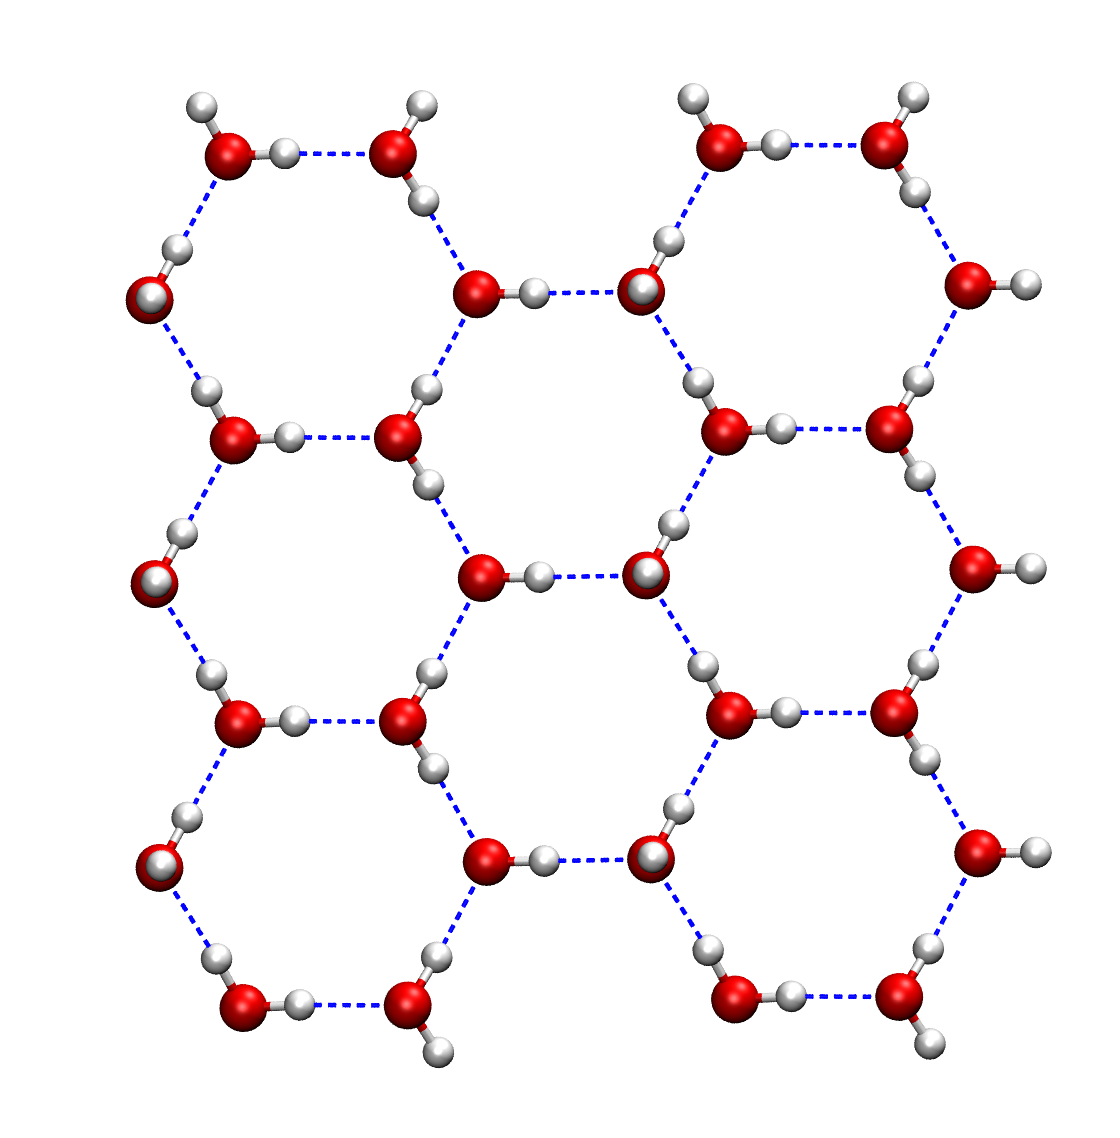
\includegraphics[width=.48\textwidth]{./img/FletcherAboveGlossyNoCueing.png}
\caption{The Fletcher surface. Hexagonal O (red) structure with vertical lines 
of identical H (white) orientation. H-bonds are indicated by dashed blue lines.
The O atoms are not all in the same plane.}
\label{Fig:Ads:Fletcher}
\end{figure}

It is best understood by consindering Figure \ref{Fig:Ads:Fletcher}. Starting
from a layer of hexagonally arranged O atoms (which are not arranged on a plane but 
alteratingly above and below the plane), one can connect each O atom to its
four nearest neighbors. On these designated hydrogen bonds, H atoms can be placed close
to one of the two O atoms taking part in the bond. This leads to a multitude
of possible arrangements. Fletcher's approach is to draw parallel
lines into the lattice to group the molecules in rows. Molecules in the
same row have the same orientation. In Figure \ref{Fig:Ads:Fletcher}, these
rows can be defined by vertical lines.

This ordering comes from first considering only the surface molecules. These
have a broken hydrogen bond outward, which may or may not have a hydrogen
atom on it. When grouping those broken bonds with hydrogen atoms and those
without hydrogen atoms in alternating rows, the structure described above is
extended to the full system.

Such a crystalline surface must be considered as an idealisation. First of all,
since we are interested in an ice surface on a grain, the interaction between
the water molecules and the grain at the grain surface will surely lead to
changes in the water crystal, probably both in O position as well as in H
orientation.
Research in that respect was presented by Cabrera Sanfelix
\etal\cite{CabreraSanfelix2003} on a graphite surface, where a water dimer
adsorbed on the surface has different bond angles than the gaseous water dimer.
Therefore, an undisturbed crystalline surface will only be reasonable if the
water ice is several monolayers thick, which is unlikely since one only
encounters ``dirty'' ices in the interstellar
medium\cite{BoogertGerakinesWhittet2015}.
A second idealization is that the crystalline structure of water ice can only be true to the perfect hexagonal structure if a layer like
in Figure \ref{Fig:Ads:Fletcher} is within the crystal, i.e.\ there are more
such layers above and below. Then, there is a balance of force. If the layers
above are removed to describe a surface layer, the forces from inside the
crystal will surely deform the ideal surface layer of Figure
\ref{Fig:Ads:Fletcher}.
We will see this effect in Section \ref{Sec:Ads:Optima}.

Instead of choosing a cuboid subdomain of the Fletcher surface -- which would be more adequate
to the surface's translational symmetry -- we will consider a hemisphere as depicted in Figure
\ref{Fig:Ads:QMMM}. We do so because the surface model shall be used in future studies
to investigate reactions. These depend on energy dissipation processes throughout the
surface, which will propagate spherically from a reaction site. The symmetry of the model
is chosen to be adequate to that, with the designated reaction site at the
central ring.

\subsubsection{The QM/MM Region}
\label{Sec:Ads:QM/MM}
%% CHECK: what is prismatic surface? Thing in Fletcher?
%\tikzsetexternalprefix{TikzPics/Adsorption/}
%\tikzsetnextfilename{Fig.Ads.QMMM}

\begin{figure*}[ht]
\centering
%\newline
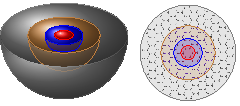
\includegraphics[width=\textwidth]{TikzPics/TikzCreation/SurfaceQMMM/SurfaceQMMMAside.pdf}
\newline
%\caption{The QM/MM division of the Fletcher surface. The upper picture shows the surface from above,
%the picture below is a schematic representation. The gray and the brown area make up the MM region,
%where water molecules are described by the $\tip$ potential. In the gray region, they are frozen. 
%The blue and brown region make up the QM region. Atoms in the blue region are described by the
%$\tzvp$ basis set. The central ring in the red region uses the $\tzvpd$ basis set.}
\caption{The QM/MM decomposition of the Fletcher surface. The picture to the right shows the surface from above,
the picture to the left is a schematic representation. The gray and the brown area make up the MM region,
where water molecules are described by the $\tip$ potential. In the gray region, they are frozen. 
The blue and red region make up the QM region. Atoms in the blue region are described by the
$\tzvp$ basis set. The central ring constituting the red region uses the $\tzvpd$ basis set.}
\label{Fig:Ads:QMMM}
\end{figure*}

%% NUMBERS:
%             ATM -  MOL
%  ALL:       3453 - 1151
%  ACTIVE:     783 -  261
%  FROZEN:    2670 -  890
%  QM:         108 -   36
%  CENTRAL:     36 -    6
%  ACTIVE MM:  675 -  225
%  MM:        3345 - 1115
We start from an infinite fully-ordered water $I_h$ crystal with a Fletcher
surface. We choose a normal basal surface as in Figure \ref{Fig:Ads:Fletcher},
not a prismatic surface. We define a central ring, that is one of the hexagonal
water rings of the surface. We take a hemispherical cut of radius $25~\Ang$
centered at the center of mass of the central ring. The hemispherical cut does
not separate $\hto$ molecules internally, instead an $\hto$ molecule is fully
incorporated in the system if its O atom is within the cutoff radius. The full
number of QM/MM water molecules in the system is 1151, with 1151 O atoms and
2302 H atoms.

The decomposition into QM/MM domains is described in Figure \ref{Fig:Ads:QMMM}.
At a sphere of radius $8~\Ang$ we separate the system into two domains. The
domain within this sphere is the QM domain and the domain outside of it
is the MM domain. 
The QM region then contains three layers of molecules. On the surface layer,
there is the central hexagonal ring of water molecules and the six
rings adjacent to it. The second layer has a water ring and the six
molecules forming hydrogen bonds with the O atoms of the ring. On 
the third layer, there is only one ring left. This would total
to 24+12+6=42 QM molecules. However, the QM description is only
necessary for regions where chemistry takes place. In our study,
this will all happen close to the surface layer. Therefore, going three
layers deep with the QM domain is not necessary and the the six
atoms of the lowest ring are also treated by MM. This makes the system slightly
less symmetric, but for the problems discussed here, the decrease in
computation time is enough to make up for that: calculations with 42 QM molecules
take on average 1.4 times as long as calculations with 36 QM molecules.
Therefore, we decide on a total of 36 QM molecules. Of these, only the central ring at
the surface is described by the $\tzvpd$ basis set, the rest
uses the $\tzvp$ basis set. 

As for the MM domain, it is again separated at $15~\Ang$ of the system center.
Those molecules within that radius can change their position (active molecules) in the optimisations we
later carry out. The rest of the MM molecules is fixed in position (frozen molecules) to yield
%% CHECK: envelope? shell?
boundary conditions. The $10~\Ang$ thick envelope of frozen molecules may not be
necessary as a boundary, but on the other hand it has virtually no effect on
computation time to include these additional MM atoms, and if necessary they
can beturned into further active atoms. There is a total of 1115 MM molecules,
of which 225 are active MM molecules and 890 frozen MM molecules.

The geometry of the original Fletcher surface has to be changed to fit the requirements
of the $\tip$ potential. In the original formulation the hydrogen atoms
are placed directly on the hydrogen bonds, that is connecting lines between each oxygen atom
and its four nearest neighbors. This process yields bond angles of $109.50\degree$
with a in principle variable bond length. The latter can be easily adjusted
to the $\tip$ requirements by simple stretching. This does not change the bond angles which
are still in disagreement with the bond angles of the $\tip$ potential
fixed at $104.52\degree$. This is mended by simply taking a perfect
Fletcher surface with adjusted bond lenghts $\abs{\r_{\te O - \te H1}}=\abs{\r_{\te O - \te H2}}=0.9572~\Ang$
and changing the angles to the $\tip$ value while maintaining
the orientation of the water dipole moment, that is the vector $\r_{\te O - \te H1}+\r_{\te O - \te H2}$
stays the same for each molecule. This means symmetrical bending of all bond angles with
respect to the dipole moment.

We must also remark on the MM force field used for adsorbates. Since our QM
region is rather big, we assume that the MM parameters for the adsorbates are
of minor importance if they stay above the central ring, but they should still
be chosen sensible. We studied only adsorbates composed of H and O. We decided on
an isolated description of the atoms in the adsorbate, with the $\tip$ LJ
potential according to atomic species and zero electric point charge. Since the
interaction of atoms within the adsorbate molecule is described by QM alone and
is independent of the coupling, this approach seems sensible. The water LJ
parameters should still be reasonable for the isolated atoms.
Only the point charges may become a greater source of error if the atoms
leave the central ring and get closer to the MM region.

\subsubsection{Setting Up the Model}

Now we talked about how to define the surface geometry and how to decompose
the system into QM and MM domains. To give guidance for a general approach to
set up a surface model, we want to repeat the steps we took.

\begin{enumerate}
  \item \textbf{Geometry.} Set up the lattice for oxygen atoms with hexagonal
  rings. Include the hydrogen atoms to arrive at the perfectly ordered Fletcher
  surface. If desired, this ordered surface can lose some order by changing the
  hydrogen orientation. It may be even further disordered by a short molecular
  dynamics calculation applying a classical force field and a finite
  temperature, which should lead to some form of ASW. When the surface satisfies the
  requirements, take a hemispherical cut. You can then add adsorbates or 
  perform other manipulations to adjust the system to your requirements.
  \item \textbf{Subdomains.} Select QM atoms and MM molecules. Divide
  the MM molecules into frozen and active molecules.
  \item \textbf{Force field.} Decide on a force field for the MM region.
  We used $\tip$ and believe that the details of the force field have only
  a minor impact on the result of the calculation due to the large
  QM region, but for smaller QM regions, its effect may be more considerable.
  Note that there are also force field parameters required for the adsorbates.
  \item \textbf{DFT.} Decide on the details of your DFT calculations. Our
  benchmark favours $\tzvpd$, therefore we recommend a $\tzvp$/$\tzvpd$ basis
  set and the functionals discussed at the end of Section \ref{Sec:Bench}.
  \item \textbf{QM/MM.} Set up the communication between QM and MM region. Note
  that you may require MM parameters for your QM atoms and that on the other
  hand your QM calculations should support point charges.
\end{enumerate}
Following this approach was very easy for us, since we used the
ChemShell interface. It supports a QM/MM interface where the QM and MM
theories can be defined independently of each other. They are then coupled to
yield a hybrid theory, which is given to $\dlfind$ alongside the initial geometry.

\subsection{First Geometry Optimisations}
\label{Sec:Ads:Optima}

To verify the agreement between the theoretically assumed Fletcher surface and the
methods we want to use, we calculated RMSD values \eqref{Bench:RMSD} between
the ideal Fletcher surface and the surface after QM/MM optimisation.
Note that the factor $\frac 1 M$ in \eqref{Bench:RMSD} is not defined by the
full number of QM/MM atoms in the system but by the number of active QM/MM atoms.

% Table generated by Excel2LaTeX from sheet 'Tabelle1'
\begin{table}[t]
  \centering
  \caption{RMSD values for the \ep{all classical} calculation with $\tip$ and
  QM/MM calculations with different functionals. Deviations to perfect Fletcher
  surface, $\tip$ optimised surface and $\btlyp$ QM/MM optimised surface,
  respectively.}
%       \begin{tabular}{lr|lr}
%     \tip  & \multicolumn{3}{l}{0.179 $\Ang$} \\[.2 pt]
%     \hline
%     \hline
%     \bhlyp & 0.182 $\Ang$ & \pw\dt & 0.187 $\Ang$\\
%     \btlyp & 0.183 $\Ang$ & \pbez & 0.193 $\Ang$\\
%     \pw   & 0.183 $\Ang$ & \tpssh & 0.191 $\Ang$ \\[.2 pt]
%     \hline
%     \end{tabular}
    \begin{tabular}{l|rrr}
    & to Fletcher & to $\tip$ & to $\btlyp$ \\[.2 pt]
    \hline
   % \tip  & 0.179 $\Ang$ \\[.2 pt]
    \tip & 0.179 $\Ang$ & 0.000 $\Ang$ & 0.101 $\Ang$ \\
\btlyp & 0.183 $\Ang$ & 0.101 $\Ang$ & 0.000 $\Ang$ \\
\bhlyp & 0.182 $\Ang$ & 0.096 $\Ang$ & 0.010 $\Ang$ \\
\pbez & 0.193 $\Ang$ & 0.103 $\Ang$ & 0.031 $\Ang$ \\
\tpssh & 0.191 $\Ang$ & 0.103 $\Ang$ & 0.025 $\Ang$ \\
\pw & 0.183 $\Ang$ & 0.102 $\Ang$ & 0.013 $\Ang$ \\
\pw\dt & 0.187 $\Ang$ & 0.101 $\Ang$ & 0.015 $\Ang$ \\
\hline
    \end{tabular}
  \label{Tab:Ads:RMSD.Methodcompare}%
\end{table}%

Data for the RMSD values are presented in Table \ref{Tab:Ads:RMSD.Methodcompare}. 
We include the pure MM optimisation with $\tip$. Generally, the results can be
considered to be good. For all systems, the same effect is visible: the active
$\hto$ molecules sink slightly into the surface. We did already have reasons to
expect that, as explained in Section \ref{Sec:Ads:Model}.
%This can be expected, since
%the initial geometry is gained by cutting a perfect crystal at a plain, so the molecules
%that are now at the surface do not feel the attractive hydrogen bonds of the removed
%molecules anymore and move closer to the remaining molecules within the surface. 
This initial sinking in process leads to an RMSD of less than $0.2~\Ang$, and
the displacement is stronger the further a molecule is away from the frozen molecule region. Below
the surface layer, the displacements due to this effect are not very strong.

The RMSD among the DFT optima is very small, they deviate from the
$\btlyp$ optimum geometry by an RMSD of $0.031~\Ang$ and less. This is small
compared to the $\te O - \te H$ separation of $0.98~\Ang$ and the $\te O - \te
O$ separation of around $2.70~\Ang$. Even those functionals we excluded in the
benchmark yield optimum geometries within boundaries of an RMSD of $0.063~\Ang$ to $\btlyp$. Between the functionals of Table \ref{Tab:Ads:RMSD.Methodcompare} and the $\tip$ potential,
there is an RMSD of around $0.1~\Ang$. The source of this deviation is that the
DFT water does not have the $\anghoh$ bond angle restriction that $\tip$ water
has to satisfy.

We can therefore say that the QM/MM descriptions we decided on all find an
optimum geometry that is close enough to the ideal Fletcher geometry. 

%% Next part necesary?
\tikzsetexternalprefix{TikzPics/Adsorption/}
\tikzsetnextfilename{Fig.Ads.QMMMConvergence}
\begin{figure}[h]
\centering
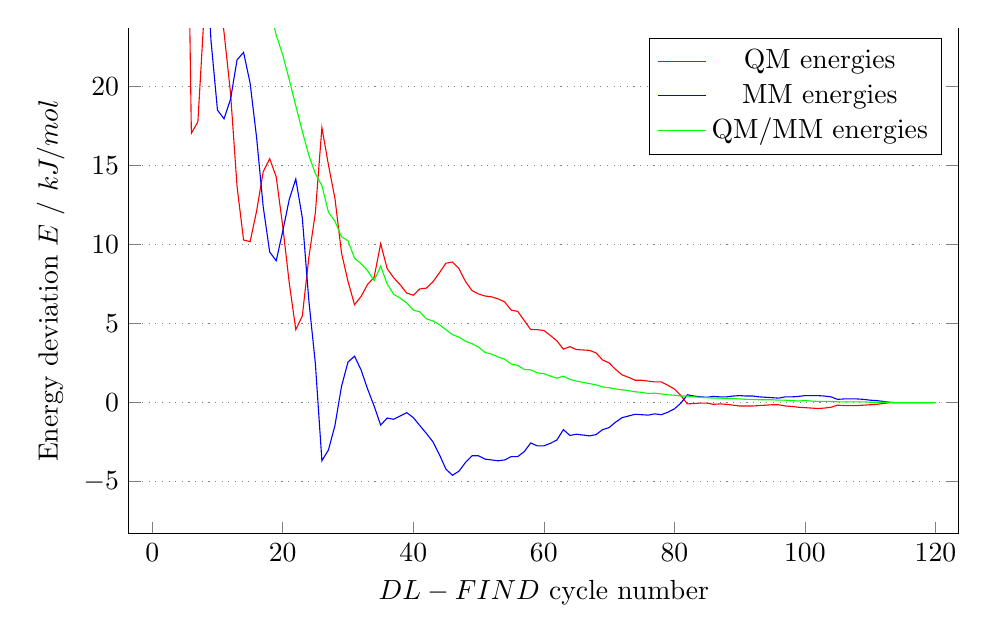
\begin{tikzpicture}
 \begin{axis}[
    height=8cm,
    width=\linewidth,
    axis x line*=bottom,
    enlarge x limits=0.03,
    xmin=0,
    xmax=120,
    enlarge y limits=0.15,
    ymax=20,
    xtick={0,20,40,60,80,100,120},
    ylabel={Energy deviation $\Dl E$ / $\kmo$},
    xlabel={$\dlfind$ cycle number},
    grid style={dotted,gray},
    ymajorgrids=true,
    ]
\addplot[red] coordinates {(0,225.924275) (1,221.644710) (2,187.276915) (3,138.232575) (4,72.201250) (5,45.421150) (6,17.039495) (7,17.774635) (8,24.942250) (9,27.488985) (10,26.543805) (11,23.445715) (12,19.586230) (13,13.678855) (14,10.291960) (15,10.186940) (16,12.129810) (17,14.597780) (18,15.437940) (19,14.282720) (20,11.158375) (21,7.561440) (22,4.620880) (23,5.487295) (24,9.189250) (25,12.024790) (26,17.407065) (27,15.044115) (28,12.917460) (29,9.478055) (30,7.666460) (31,6.196180) (32,6.721280) (33,7.482675) (34,7.929010) (35,10.055665) (36,8.480365) (37,7.902755) (38,7.456420) (39,6.931320) (40,6.800045) (41,7.193870) (42,7.246380) (43,7.640205) (44,8.217815) (45,8.821680) (46,8.900445) (47,8.480365) (48,7.666460) (49,7.088850) (50,6.878810) (51,6.747535) (52,6.695025) (53,6.563750) (54,6.379965) (55,5.854865) (56,5.776100) (57,5.198490) (58,4.620880) (59,4.620880) (60,4.568370) (61,4.253310) (62,3.911995) (63,3.386895) (64,3.544425) (65,3.360640) (66,3.334385) (67,3.308130) (68,3.150600) (69,2.704265) (70,2.520480) (71,2.100400) (72,1.759085) (73,1.601555) (74,1.417770) (75,1.417770) (76,1.365260) (77,1.312750) (78,1.312750) (79,1.102710) (80,.866415) (81,.446335) (82,-.078765) (83,-.052510) (84,-.026255) (85,-.026255) (86,-.105020) (87,-.078765) (88,-.105020) (89,-.157530) (90,-.210040) (91,-.210040) (92,-.210040) (93,-.183785) (94,-.157530) (95,-.131275) (96,-.131275) (97,-.210040) (98,-.236295) (99,-.288805) (100,-.315060) (101,-.341315) (102,-.367570) (103,-.341315) (104,-.288805) (105,-.157530) (106,-.183785) (107,-.183785) (108,-.183785) (109,-.157530) (110,-.131275) (111,-.105020) (112,-.052510) (113,0) (114,0) (115,0) (116,0) (117,0) (118,0) (119,0) (120,0) };
\addplot[blue] coordinates {(0,42.979435) (1,42.506845) (2,37.518395) (3,31.427235) (4,39.408755) (5,48.598005) (6,58.548650) (7,46.471350) (8,30.403290) (9,22.946870) (10,18.509775) (11,17.958420) (12,19.192405) (13,21.686630) (14,22.159220) (15,20.216350) (16,16.750690) (17,12.418615) (18,9.530565) (19,8.979210) (20,10.843315) (21,12.864950) (22,14.151445) (23,11.683475) (24,6.458730) (25,2.467970) (26,-3.675700) (27,-2.993070) (28,-1.444025) (29,1.023945) (30,2.572990) (31,2.940560) (32,2.074145) (33,.866415) (34,-.210040) (35,-1.417770) (36,-.971435) (37,-1.050200) (38,-.840160) (39,-.630120) (40,-.945180) (41,-1.444025) (42,-1.942870) (43,-2.467970) (44,-3.281875) (45,-4.200800) (46,-4.594625) (47,-4.332075) (48,-3.780720) (49,-3.360640) (50,-3.360640) (51,-3.570680) (52,-3.623190) (53,-3.675700) (54,-3.623190) (55,-3.413150) (56,-3.413150) (57,-3.098090) (58,-2.546735) (59,-2.730520) (60,-2.730520) (61,-2.572990) (62,-2.362950) (63,-1.706575) (64,-2.074145) (65,-1.995380) (66,-2.047890) (67,-2.100400) (68,-2.021635) (69,-1.706575) (70,-1.575300) (71,-1.233985) (72,-.945180) (73,-.840160) (74,-.735140) (75,-.761395) (76,-.787650) (77,-.708885) (78,-.761395) (79,-.603865) (80,-.393825) (81,-.026255) (82,.498845) (83,.420080) (84,.367570) (85,.341315) (86,.393825) (87,.367570) (88,.367570) (89,.420080) (90,.446335) (91,.420080) (92,.420080) (93,.367570) (94,.341315) (95,.315060) (96,.288805) (97,.367570) (98,.367570) (99,.393825) (100,.446335) (101,.446335) (102,.446335) (103,.420080) (104,.367570) (105,.210040) (106,.236295) (107,.236295) (108,.236295) (109,.210040) (110,.157530) (111,.131275) (112,.078765) (113,.026255) (114,0) (115,0) (116,0) (117,0) (118,0) (119,0) (120,0) };
\addplot[green] coordinates {(0,268.903710) (1,264.151555) (2,224.795310) (3,169.659810) (4,111.610005) (5,94.019155) (6,75.588145) (7,64.245985) (8,55.345540) (9,50.435855) (10,45.053580) (11,41.404135) (12,38.778635) (13,35.365485) (14,32.451180) (15,30.403290) (16,28.880500) (17,27.016395) (18,24.968505) (19,23.261930) (20,22.001690) (21,20.426390) (22,18.772325) (23,17.170770) (24,15.647980) (25,14.492760) (26,13.731365) (27,12.051045) (28,11.473435) (29,10.502000) (30,10.239450) (31,9.136740) (32,8.795425) (33,8.349090) (34,7.718970) (35,8.637895) (36,7.508930) (37,6.852555) (38,6.616260) (39,6.301200) (40,5.854865) (41,5.749845) (42,5.303510) (43,5.172235) (44,4.935940) (45,4.620880) (46,4.305820) (47,4.148290) (48,3.885740) (49,3.728210) (50,3.518170) (51,3.176855) (52,3.071835) (53,2.888050) (54,2.756775) (55,2.441715) (56,2.362950) (57,2.100400) (58,2.074145) (59,1.890360) (60,1.837850) (61,1.680320) (62,1.549045) (63,1.680320) (64,1.470280) (65,1.365260) (66,1.286495) (67,1.207730) (68,1.128965) (69,.997690) (70,.945180) (71,.866415) (72,.813905) (73,.761395) (74,.682630) (75,.656375) (76,.577610) (77,.603865) (78,.551355) (79,.498845) (80,.472590) (81,.420080) (82,.420080) (83,.367570) (84,.341315) (85,.315060) (86,.288805) (87,.288805) (88,.262550) (89,.262550) (90,.236295) (91,.210040) (92,.210040) (93,.183785) (94,.183785) (95,.183785) (96,.157530) (97,.157530) (98,.131275) (99,.105020) (100,.131275) (101,.105020) (102,.078765) (103,.078765) (104,.078765) (105,.052510) (106,.052510) (107,.052510) (108,.052510) (109,.052510) (110,.026255) (111,.026255) (112,.026255) (113,.026255) (114,0) (115,0) (116,0) (117,0) (118,0) (119,0) (120,0) };
\legend{QM energies, MM energies, QM/MM energies};
 \end{axis}
\end{tikzpicture}
\caption{The QM/MM energy changes during a typical optimisation. The 
energies are deviations from their value at the optimum geometry.
Functional: $\bhlyp$.}
\label{Fig:Ads:QMMMConvergence}
\end{figure}

We can also compare the behaviour of the QM and MM part during the optimisation
process starting at the initial crystalline geometry. Figure \ref{Fig:Ads:QMMMConvergence}
gives a typical example with the $\bhlyp$ functional. The QM, MM and
QM/MM energies are given as differences to their values at the energy minimum.
At the perfectly crystalline system, the energy difference is too high for the
plot axis, it goes up to $226~\kmo$ for the QM part and $43~\kmo$ for the MM part. 
%This is again an implication that the actual
%optimum geometry has to be tighter bound and that the effect is strongest for
% the QM region, although the high energies in the QM region must also be due to the
%physically wrong $\tip$ geometry.
After the first few iterations, one can see
that the energy changes in both domains are of the same order of magnitude. The
overall energy seems to converge more or less smoothly. There is a codependence
visible where a more attractive interaction in the MM region is accompanied by
a less attractive interaction in the QM region and vice versa. We take this as
an implication that the interaction between the two region works well and that
neither one of them is outbalanced by too strong energy gradients in the other
one. We also see this as an indication that active MM atoms should be included
in a geometry optimization to allow proper deformations of the QM region.

\subsection{ZPE Corrections}
\label{Sec:Ads:ZPE}

Now we have established a model that should be able to describe $\tripo$, 
H and $\hto$ adsorption to some satisfaction. We can compute optimum geometries
and their energies for different adsorbates and gain the adsorption energy
according to \eqref{Theo:AdsorptionEnergy}. Before we do so, it is necessary
to give a few words on the ZPE correction in this case.

With the QM/MM coupling, we can still compute analytical
gradients\cite{VersluisZiegler1988}, but analytical Hessians are
no longer available. There is no way around computing finite differences, so
two atomic diplacements per coordinate per atom, leading to six displacements
per atom. Computations for more complicated systems, especially $\sur\hot$
calculations with their doublet character, require a sensible choice of atoms
to be displaced. On the other hand of course, enough atoms should be displaced
such that the finite difference maintains good results.

Obviously, the MM atoms do not need to be displaced. If their electrons are not
described by quantum mechanics then neither should their atomic cores get a
quantum mechanical correction. As for the QM region, we come back to the argument that
the atoms relevant to adsorption are the central ring of six $\hto$ molecules plus adsorbate,
that is those atoms that we describe with the $\tzvpd$ basis set. The idea
here is that when an adsorbate comes into the system and is adsorbed within the
central ring, then its impact on the vibrational ground state of the system
will mostly affect the atoms within the ring. The effect on atoms further
away should be considerably less. However, the question if the cutoff for this effect
should only include the central ring must be further investigated. The
upshot is obvious: With $M$ being the number of atoms in the adsorbate, these $18+M$ atoms
need $108+6M$ displacements (plus one initial geometry). This is much less than
the original $648+6M$ displacements for $108+M$ QM atoms.

We will call this selective correction the $\zpering$ correction in contrast to
the $\zpeall$ correction for all QM atoms. Corresponding energies are then called
$\ering$ and $\eall$, respectively, and the corrections are $\Dl\eall$ and $\Dl\ering$. 

We can compare the two corrections in the next section.


%% CHECK: Formation energies gegeneinander plotten? Eigentlich nicht sinnvoll,
%   da die QM Geometrien ja nicht unabhängig von den MM Geometrien sind.

\subsection{Adsorption}
\label{Sec:Ads:Adsorption}
\newcommand\avg{\enmat{E_{\te {avg}}^{\te{ads}}}}
%If we assume the $\zpeall$ correction 
%to be accurate, we can evaluate the $\zpering$ correction when comparing
%results for the $\btlyp$ functional in Table \ref{Tab:Ads:AdsB3lyp}.
Of the molecules relevant in Section \ref{Sec:Gas}, we examine adsorption
%% CHECK: Conformation wirklich richtig? Chemisorption richtig? Unterschiede
%   zu Physisorption behandeln?
energies for all species but $\singo$, since it is chemisorbed by the surface
to form some conformation of $\htot$. This is a result of the barrierless
and very exothermic reaction \mbox{$\hto+\singo\chemar\htot$}, as described in
\eqref{Gas:H2O+O->H2O2}.

%% CHECK: Vllt lieber die Corrections als die Energiewerte?
%\renewcommand\eads[1]{E_{\sur\te X}^{\te{ads}{#1}}}
\begin{table}[htb]
  \caption{Different choices for the ZPE correction. For a reference, the corresponding 
  adsorption energies are given for the $\btlyp$ functional. All energies in $\kmo$.}
  \centering
    \begin{tabular}{l|rrrr}
       & & & & \\[-10pt]
     & $E_{\btlyp}$   & $\Dl\eall_{\btlyp}$ & $\Dl\ering_{\btlyp}$ & $\Dl\ering_{\pbez}$ \\[2pt]
    \hline
       & & & & \\[-10pt]
    $\sur\te{H}$ & $-$1.71 & 5.03  & 3.28  & 2.84 \\
    $\sur\htw$ & $-$2.65 & 8.42  & 6.80  & 6.81 \\
    $\sur\hto$ & $-$48.01 & 15.98 & 14.84 & 14.45 \\
    $\sur\htot$ & $-$41.76 & 9.28  & 10.09 & 9.51 \\
    $\sur\ho$ & $-$44.99 & 13.60 & 12.11 & 12.05 \\
    $\sur\hot$ & $-$65.48 & 13.17 & 11.66 & 11.59 \\
    $\sur\tripo$ & $-$16.17 & 2.69  & 3.35  & 3.04 \\
    $\sur\singot$ & $-$8.41 & 2.46  & 3.86  & 4.96 \\
    $\sur\tripot$ & $-$2.62 & 3.06  & 3.90  & 3.86 \\[2pt]
    \hline
    \end{tabular}%
% \begin{tabular}{l | r|r|r|}
% & & & \\[-10pt]
%     & \ph{$^{\zpeall}$}$\eads{}$ & $\eads{,\zpering}$ & $\eads{,\zpeall}$ \\[2pt]
%     \hline
%        & & & \\[-10pt]
%     $\sur\te H$ & -1.69 & 1.62  & 3.43 \\
%     $\sur\te H_2$ & -2.65 & 4.19  & 5.91 \\
%     $\sur\hto$ & -48.00 & -33.14 & -32.06 \\
%     $\sur\htot$ & -41.76 & -31.62 & -32.39 \\
%     $\sur\te{HO}$ & -44.98 & -32.85 & -31.39 \\
%     $\sur\te{HO}_2$ & -65.48 & -53.79 & *** \\
%     $\sur^3\te O$ & -16.15 & -12.77 & -13.38 \\
%     $\sur^1\te O_2$ & -8.42 & -4.50 & -5.76 \\
%     $\sur^3\te O_2$ & -2.48 & 1.49  & 0.83 \\[2pt]
%     \hline
%     \end{tabular}
  \label{Tab:Ads:AdsB3lyp}%
\end{table}%

%% CHECK: Wird das noch was?
%Also note that the $\hot$ calculation did not finish within the six days
%of computation on the JUSTUS cluster for the $\zpeall$ correction. It did
%only finish 307 of 333 displacements.  

Before discussing adsorption data, we want to discuss the relevance of the
$\zpe$ correction and the differences between $\zpeall$ and $\zpering$
as well as the differences between the $\zpering$ correction for $\btlyp$ and
$\pbez$, which we hope to represent the variability of the
$\zpe$ correction for different functionals.

In general, the value of the correction term varies from
adsorbate to adsorbate. All three corrections lie roughly between $2$
and $16~\kmo$. That makes them -- if there is no cancellation
of error of some other sort -- necessary for the correct description
of adsorption processes, since the uncorrected adsorption energies
themselves lie between $-1.71$ and $-65.48~\kmo$. Usually, the ZPE correction
is between $15\%$ and $30\%$ of the uncorrected energy. The exceptions are
$\sur{\te H}$, $\sur{\htw}$ and $\sur{\tripo}$, which we will discuss later. The
value of the ZPE correction is also typically greater than the variation of the
uncorrected adsorption energy of different functionals, as we can see when
comparing to Table \ref{Tab:Ads:AdsForFuncs}.

The $\zpeall$ and $\zpering$ energies
do not deviate strongly in absolute value, all of them less than $2~\kmo$
and all but $\sur$H and $\sur$HO by less than $1.5~\kmo$. All corrections are
positive.
% and in most cases the deviation is of less than 25\% between
%the two. Only for $\sur$H and $\sur^1\ot$ the deviations are greater than 35\%.
It seems safe to say that the $\zpering$ correction may not be extremely
close to the $\zpeall$ correction, but it shows the same qualitative
behaviour. 
%And since there is no knowing whether or not $\zpeall$ is
%accurate either, 
It seems alright to use the correction of the smaller system with an error to
the correction for the full system of $\pm 2~\kmo$.

Comparing the correction terms for $\btlyp$ and $\pbez$, we generally find
good agreement. With the exception of $\sur\singot$, the energies
differ by less than $0.6~\kmo$.
%The case of $\sur^1\ot$ is also
%interesting because it is the only case where the $\pbez$ correction
%predicts a greater value than the $\btlyp$ correction.
Given the uncertainty between $\zpering$ and $\zpeall$, the differences
between the  $\pbez$ correction and the $\btlyp$ correction are negligible.
It seems reasonable to generalize what we already discovered for the gas
phase result of Section \ref{Sec:Gas}: the ZPE correction does
not change greatly between different functionals. We will therefore
use the $\zpeall$ correction for the $\btlyp$ functional for all
following data.

Talking about the differences between $\zpe$ corrected adsorption energies
and those without correction, there are the interesting cases of 
$\sur$H, $\sur\htw$ and $\sur\tripot$. In all three cases, the uncorrected
$E$ predicts weakly attractive interaction, while the corrected $\eall$
and $\ering$ both predict repulsive interaction. That means that
the binding site found by the uncorrected DFT method is probably not the
desired optimum.
In such a case, it would of
course be interesting whether there is an optimum geometry for the $\zpe$
corrected functional that is still attractive. One should assume so,
since it would seem unphysical if the surface and one of the
molecules would repel one another. The problem here may be more the
$\btlyp$ functional than the $\zpe$ correction alone. Due to the computational
cost of a single ZPE correction, an optimization on a ZPE corrected
PES will be very difficult to achieve.

Still, the $\zpe$ correction in such a weakly adsorbed case is probably
erroneous since the minimum is probably very shallow. This means
that approximating the PES by a harmonic potential does not reproduce the PES
correctly.

This result implies that the adsorbates $\sur{\te H}$, $\sur{\htw}$ and
$\sur{\tripot}$ are only very weakly bound to the surface in this 0 K limit.

% We can further evaluate the significance of the ZPE correction by comparing
% it to the variation in (uncorrected) adsorption energy among 
% the different functionals.

\newcommand\tableskip{\hskip 0pt}
\newcommand\leftattable{\raggedright\hskip 53pt}
\newcommand\righttable{\raggedleft}
\newcommand\righttablestop{\hskip-53pt}
\newcommand\footnotebox{\tableskip\tableskip\makebox[.93\textwidth][r]}
%% CHECK: b3lyp muss ja evtl nicht nochmal a	usgegraben werden. Dafür
% vllt pw6b95.
%% CHECK: More Experiments?
%% CHECK: Deviation from average value? 
% Table generated by Excel2LaTeX from sheet 'Tabelle1'
\begin{table*}[ht]
  \centering
  \caption{Comparison of adsorption energies for different density functionals. All
  energies are given with $\zpeall$ correction for $\btlyp$. $\pws$ is shorthand
  for $\pw$. Energies can be compared to the average $\avg$ and experimental data.
  MAD, MIN, MAX and MEAN are give with respect to $\avg$.
  Energies in $\kmo$.}
    %\begin{tabular}{l|L{2cm}L{2cm}L{2cm}L{2cm}L{2cm}}
    \begin{tabular}{l|rrrrrr|r|r}
    & & & & & & & & \\[-10pt]
          & \btlyp & \bhlyp & \pbez & \tpssh & \pws & \pws\dt & $\avg$ &experimental, $E_\te{des}$\\[2pt]
    \hline
       & & & & &  & & & \\[-10pt]
    $\sur\te{H}$ & 3.32  & 3.77  & 3.37  & -5.05 & 3.29  & 1.27 & 1.66 & \\
    $\sur\htw$ & 5.77  & 5.11  & 3.57  & 4.55  & 4.65  & 2.47 & 4.35 & \\
    $\sur\hto$ & $-$32.03 & $-$35.07 & $-$36.90 & $-$30.92 & $-$33.51 & $-$41.17 & $-34.93$ & $-$$48.00\pm0.50$\fakefna\\
    $\sur\htot$ & $-$32.47 & $-$35.99 & $-$37.64 & $-$31.04 & $-$34.85 & $-$44.33 & $-36.05$ &\\
    $\sur\ho$ & $-$31.39 & $-$32.88 & $-$35.69 & $-$31.10 & $-$32.78 & $-$39.66 & $-33.92$ & $-$$13.77$ to $-$$39.58$\fakefnb\\
    $\sur\hot$ & $-$52.30 & $-$49.10 & $-$56.97 & $-$54.10 & $-$51.08 & $-$57.80 & $-53.56$ & \\%  $13.80\pm0.50$\fakefnb,\\
    %% CHECK: This value is only for the bare silicate
    %& & & & & & & $15.38\pm0.75$\fakefnb \\
    $\sur\tripo$ & $-$13.48 & $-$5.16 & $-$11.25 & $-$13.22 & $-$12.85 & $-$18.13 & $-12.35$ &
    $-13.80\pm0.50$ or $-15.38\pm 0.75$\fakefnc \\
    $\sur\singot$ & $-$5.95 & $-$7.51 & $-$11.44 & $-$9.44 & $-$7.44 & $-$12.53 & $-9.05$ & \\
    $\sur\tripot$ & 0.45  & $-$0.65 & $-$1.52 & $-$0.52 & 26.68 & 7.04 & $-0.56^\dagger$ & $-$7.52\fakefnd\\[2pt]
    \hline \hline
    & & & & & &  \\[-10pt]
    MAD   & 2.06  & 1.93  & 1.74  & 2.29  & 4.17  & 4.85   \\
    MIN   & -1.13 & -0.14 & -3.42 & -6.72 & -0.50 & -8.28  \\
    MAX   & 3.58  & 7.19  & 1.71  & 5.02  & 27.23 & 7.60   \\
    MEAN  & 1.81  & 1.88  & -1.12 & 0.40  & 4.06  & -3.16  \\
    \end{tabular}
    \\[5pt]
    \footnotebox{
    \fakefna\footnotesize Adsorption on Au grain covered in crystalline water. For other grain materials between $42.15$ and $49.79~\kmo$. Fraser $\etal~$ 2001\cite{Fraser2001}}\\
    %% CHECK: Überhaupt relevant, wenn nicht auf asw oder crystalline?
    \footnotebox{
    \fakefnb\footnotesize Adsorption on an amorphous silicate. He, Vidali 2014 \cite{HeVidali2014}}\\
    %% CHECK: Paper anschauen, LESEN
    \footnotebox{
    \fakefnc\footnotesize Adsorption on porous amorphous water ice and amorphous silicate, respectively. He $\etal~$ 2015 \cite{He2015}}\\
    \footnotebox{
    \fakefnd\footnotesize Adsorption on an amorphous silicate. He, Jing, Vidali 2014 \cite{HeJingVidali2014}}\\
    \footnotebox{
    $^\dagger$\footnotesize Average excluding both $\pws$ and $\pws\dt$.}\\
    %\makebox[10cm]{\ragggedleft Text}\\
    %\leftattable Text\\
    %\righttable\righttablestop Text
    %\raggedleft\fakefna\footnotesize Value for an Au grain. Value for other substrates between $42.15$ and $49.79~\kmo$.
  \label{Tab:Ads:AdsForFuncs}%
\end{table*}%

Let us now turn to Table \ref{Tab:Ads:AdsForFuncs}, where ZPE corrected adsorption
energies are given. Where there is experimental data available, it is given
in the last column. So far, not many studies exist on measuring 
adsorption under interstellar conditions. We therefore also include some data
for $\ho$, $\tripo$ and $\singot$ adsorption on bare amorphous silicates, which were gathered in order to
gain a better understanding of water ice formation on bare silicates \cite{HeVidali2014,HeJingVidali2014}.
Other data include $\hto$ adsorption on an Au surface covered in crystalline water
%% CHECK: Es müsste \tripot sein, da Bildungsenergie für \singot größer ist als für \tripot
%    Nein, ich glaube nicht, da die Adsorptionsenergie stärker ist für \singot, das heißt ein
%    adsorbiertes O wird eine \singot-Struktur suchen. Wahrscheinlich passiert das, bevor es desorbiert.
ice\cite{Fraser2001} and $\tripot$ adsorption on porous amorphous water ice \cite{He2015}.
%% CHECK: Wie sinnvoll ist das?
%Although the experiments on bare silicates do not quite resemble our system,
%we consider the data they provide to give good guidance since they are at least
%influenced by adsorption on the freshly formed water ice surfaces on the probes.
We have an estimation of the difference between adsorption on water ice and
on the bare grain by comparing the experimental data for $\sur\tripo$, where the difference
is below $3~\kmo$ including the error bars. While this does not have to apply to all
adsorbates, a difference of similar magnitude is at least plausible, such that
the experimental values for adsorption energies on bare grains should be a rough estimate
to the adsorption energies on water surfaces on grains.

% Also note that the experiments were measurements of the desorption energy. They are
% typically temperature-dependent. We did not include any dynamical effects into our
% computations, which means they are basically data at $0~\K$. At such low temperatures,
% the difference should  

% If we compare this data directly to the $\zpe$ corrections, we should bear in mind that the
% $\zpe$ corrections given so far are only values for the $\btlyp$ functional. It
% is however well possible that the corresponding corrections of other functionals
% are of similar magnitude, given that for many adsorbates, the adsorption energy
% does not vary too strongly between the functionals. Still, the difference
% between most attractive and most repulsive functional is often greater than
% either $\zpe$ correction. As long as there is no evidence that one
% of the functionals is more accurate than the others, the error
% from the uncertain choice of functional is of the same dimension as the error
% introduced by neglect of the $\zpe$ correction. Nonetheless, the $\zpe$
% correction should be included in calculations since it seems to introduce
% additional repulsion into the system. Especially if it does really expose
% bad choices of optimum geometry, i.e. binding sites, as for the case
% of $\sur^3\ot$ for $\btlyp$.

Table \ref{Tab:Ads:AdsForFuncs} also contains a column with average values
for each adsorbate.
For $\sur\tripot$, $\pw$ and $\pw\dt$ are excluded from the average because of
the two very unphysical values. We will use this average energy
when discussing reactions.

%% CHECK: Sehr schwammig hier.
When there is no experimental data available, we can only compare the
functionals to one another. For both $\sur\te H$ and $\sur\htw$, the
problem of repulsive interaction due to ZPE correction seems to affect
most functionals. $\tpssh$ disagrees with the others by still maintaining
a negative sign for $\sur$H, but for $\sur\htw$, all functionals agree.
This is at least an indication that the physisorption of H and $\htw$ is
very fragile and that rather oxygen and hydrogenated oxygen species
have longer residence times than hydrogen.
For $\tripot$, the case is a little puzzling. $\pw$ predicts a strong
repulsion between surface and $\tripot$, which is supported by
$\pw\dt$. This looks like an error in some computation script, however we were
unable to find such an error. We must therefore consider $\pw$
to be unreliable for $\tripot$ adsorption. The other
functionals predict very weak attraction, only $\btlyp$ predicts
a very weak repulsion. We thus infer that $\tripot$ is
probably only weakly bound to the surface, too, and must have a short
residence time.
% $^3\ot$, which was also
% critical in our discussion of the ZPE correction, is not the unanimously
% considered repulsive. The $\pw$ method predicts strong repulsion,
% which is to some extent supported by $\pw\dt$, but the rest of the functionals
% seems to still predict a weak attraction or in the $\btlyp$ case a very
% weak repulsion.

While each functional does have its ``slips'' for some adsorbates, the first four functionals of
Table \ref{Tab:Ads:AdsForFuncs} seem to be in good accord. 
For many cases, one of the two $\pw$ functionals is furthest from an average
value of all six functionals. This is especially true for O and $\ot$.
Since it is either $\pw$ or $\pw\dt$, this could be an indication
that neither the $\pw$ nor the D3 dispersion correction are universally
reliable for the study at hand.

Comparing the results to experimental findings, the agreement is more qualitative
than quantitative. As already mentioned, the systems described by experiment
differ from the idealized system we study. Most noteworthy is that the data for $\sur\hto$
is far off while the experiment yielding the results should be the one closest
to our model. The agreement would be better if we neglected $\Dl\eall=15.98$,
with extremely good results for $\btlyp$ (cf. Table \ref{Tab:Ads:AdsB3lyp}).
It is even the case that the experimental values mostly lie somewhere between
the $\zpe$ corrected energy value and the uncorrected one for many functionals.
There are a number of potential sources of error. One could be the already
discussed problem of the ZPE correction to describe shallow minima. Still,
the ZPE correction represents a physical necessity and its inclusion can not
be questioned generally.
%% CHECK: Das nötig?
Another source of error is the system's strongly
idealized geometry, which is not only due to the QM description but also to
the water geometry of the MM description, which would make it difficult to
allow for systems with distorted bond angles as described by Cabrera Sanfelix $\etal~$ 
\cite{CabreraSanfelix2003} for the case of adsorption of a water dimer on graphite.
We will come back to possible improvements to the model in the final section.

% Compared to the experimental data, the case of $\tripot$ seems to be difficult
% to describe for all functionals. They predict weak adsorption, while the data by
% He \cite{He2015}, which is for an amorphous surface, predicts adsorption
% energies around $-13.8~\kmo$. While this could be dependent on the surface
% geometry, particularly bad  

On the other hand, the broad agreement between $\btlyp$, $\bhlyp$, $\pbez$
and $\tpssh$ allows for the assumption that the energies calculated for the
model at hand may be accurate to within a few $\kmo$. Since we chose
the functionals because they were best able to describe interaction
energies in Section \ref{Sec:Bench}, this hope becomes more plausible.
However, due to their rather bad performance for O species, the $\pw$
functionals have lost some credibility.


% Again, there is no knowing 
% what results are accurate. But if a single functional does not agree well with
% the rest of them, as is the case for $\pw\dt$, one could argue that it may
% at least be a little more off than the others. Also, the result
% of repulsive $\sur^3\ot$ interaction is odd, especially since $\pw\dt$ 
% expected too attractive interaction for the $\htoo$ benchmark.

% Concerning the other four functionals, one cannot make out many patterns
% in their behavior. They agree within $\pm2.5~\kmo$ of an average value
% for half of the adsorbates, but they do not coincide well for $\sur$H, $\sur\hot$,
% $\sur^3$O and $\sur^1\ot$, either because of a single functional strongly
% disagreeing or because of all functionals predicting energies in a broader
% area. There is no thoroughly satisfactory conclusion to this. One can
% at least argue qualitatively that the results should be physically
% sensible and that the scatter of possible values could be used as an error
% bound for the actual data.

\subsection{Reactions}
\label{Sec:Ads:Reactions}

%% CHECK: Durchschnittswert in nem Bild präsentieren? Durchschnittswert wirklich clever?
\newcommand\btlyps{\enmat{\te{B3}}}
\newcommand\pbezs{\enmat{\te{PBE0}}}
\newcommand\erehyb{\enmat{\ere_{\te{hybrid}}}}
% Table generated by Excel2LaTeX from sheet 'Tabelle1'
\begin{table*}[htb]
  \centering
  \caption{Surface reaction energies with Eley-Rideal type reactions. All energies are $\zpe$ corrected with $\Dl E^{\zpeall}_\btlyp$.
  $\pws$ is short for $\pw$. The functionals most accurate for the gas-phase
  reactions are highlighted by boldface again (cf. Table
  \ref{Tab:Gas:Reactions}). The last column contains average values.
  The deviations of these are listed in the last four rows for each functional.}
    \begin{tabular}{lll|rrrrrr|r}
        & & & & & & & &\\[-10pt]
        & &    & \btlyp & \bhlyp & \pbez & \tpssh & \pws
    & \pws\dt &  \multicolumn{1}{r}{$\erehyb$}  \\[2pt]
    %& &    & \btlyp & \bhlyp & \pbez & \tpssh & \pws   & \pws\dt &  $\Dl \eall_{\btlyps}$ & $\ering_{\btlyps}$ & $\Dl \ering_{\pbez}$ \\[2pt]
    \hline 
    & & & & & & & &\\[-10pt]
        $\sur\ho$&\defskip$+\te{H}\gas$&\defskip$\chemar\sur\hto$ & $-$476.22 &
        $-$458.03 & $-$472.39 & $-$470.76 & $\bo{-480.13}$ & $\bo{-480.92}$ &
        $-$492.71
        \\
    $\sur\hto$&\defskip$+^1\te{O}\gas$&\defskip$\chemar\sur\htot$ & $-$402.54 &
    $\bo{-357.85}$ & $-$427.27 & $-$426.38 & $-$405.24 & $-$407.50 & $-344.17$
    \\
    $\sur\ho$&\defskip$+\ho\gas$&\defskip$\chemar\sur\htot$ & $-$185.12 &
    $-$137.04 & $-$194.02 & $-$187.84 & $\bo{-197.12}$ & $\bo{-200.16}$ &
    $-205.33$
    \\
    $\sur\hot$&\defskip$+\te{H}\gas$&\defskip$\chemar\sur\htot$ & $\bo{-317.22}$
    & $-$318.69 & $-$310.31 & $-$309.82 & $-$320.89 & $-$323.99 & $-343.39$ \\
    $\sur\ho$&\defskip$+^3\te{O}\gas$&\defskip$\chemar\sur\hot$ & $-$294.05 &
    $-$219.54 & $-$300.54 & $\bo{-295.71}$ & $-$296.15 & $-$296.10 & $-287.00$
    \\
    $\sur^3\te{O}$&\defskip$+\ho\gas$&\defskip$\chemar\sur\hot$ & $-$311.96 &
    $-$248.31 & $-$325.41 & $\bo{-313.50}$ & $-$316.45 & $-$318.00 & $-308.95$
    \\
%    $\sur^1\ot$&\defskip$+\te{H}\gas$&\defskip$\chemar\sur\hot$ & $-$403.80 &
    % $-$414.31 & $-$402.88 & $-$404.70 & $-$395.22 & $-$396.95 & $-367.42$ \\
    $\sur^3\ot$&\defskip$+\te{H}\gas$&\defskip$\chemar\sur\hot$ & $-$248.05 &
    $-$243.27 & $-$241.72 & $\bo{-250.31}$ & $-$268.95 & $-$256.14 & $-254.74$
    \\[2pt]
    
    \hline \hline
\multicolumn{2}{r|}{\multirow{4}{*}{$E_{\dft} - \erehyb$}} &
                            MAD   & 19.71 & 40.13 & 27.26 & 24.70 & 19.32 & 17.04 &  \\
    \multicolumn{2}{r|}{} &  MIN   & $-$58.37 & $-$13.68 & $-$83.10 & $-$82.21 & $-$61.07 & $-$63.33 &  \\
    \multicolumn{2}{r|}{} &  MAX   & 26.17 & 68.29 & 33.07 & 33.57 & 22.49 & 19.39 &  \\
    \multicolumn{2}{r|}{} &  MEAN  & 0.16  & 36.22 & $-$5.06 & $-$2.58 & $-$6.95 & $-$6.65 &  \\[5pt]
%
% \multicolumn{2}{r|}{} &    MIN   & $-$58.37 & $-$13.68 & $-$83.10 & $-$82.21 & $-$61.07 & $-$63.33 &  \\
% \multicolumn{2}{r|}{} &    MAX   & 26.17 & 68.29 & 33.07 & 33.57 & 22.49 & 19.39 &  \\
% \multicolumn{2}{r|}{} &    MEAN  & 1.05  & 37.11 & $-$4.16 & $-$1.68 & $-$6.06 & $-$5.76 &  \\[2pt]
%
% \multicolumn{2}{r|}{} &   MIN   & $-$58.37 & $-$46.72 & $-$83.10 & $-$82.21 & $-$61.07 & $-$63.33 &  \\
% \multicolumn{2}{r|}{} &   MAX   & 26.17 & 68.29 & 33.07 & 33.57 & 22.49 & 19.39 &  \\
% \multicolumn{2}{r|}{} &   MEAN  & 1.05  & 26.63 & $-$8.05 & $-$6.11 & $-$8.76 & $-$8.71 &  \\
        %\\[-10pt]
    \end{tabular}%
    %\\
    %\raggedleft\fakefna\footnotesize Correction value for $\btlyp$ calculation. Others differ in $\ho\gas$ $\zpe$ correction within $1.5~\kmo$.
  \label{Tab:Ads:React}%
\end{table*}%


With the adsorption energy data and corresponding gas-phase energies at the
$\tzvpd$ level, we can calculate reaction energies. We will only
consider reactions of the Eley-Rideal mechanism in which a molecule
from the gas phase approaches an adsorbed molecule to form
a new molecular species, as described in the introduction.
The product will for our study always be a single adsorbed molecule. With our data,
one could also investigate cases where two product molecules remain
of which none, one or both remain adsorbed on the surface.

We use ER versions of the gas-phase reactions \eqref{Gas:Reactions}, namely

\renewcommand\ronebox[1]{\makebox[1cm][l]{\enmat{#1}}}
\renewcommand\rtwobox[1]{\makebox[1.cm][l]{\ \enmat{#1}}}
\renewcommand\prodbox[1]{\makebox[1.65cm][l]{\enmat{#1}}}
\begin{subequations}
\begin{align}
   \label{Surf:HO+H->H2O}
   \ronebox{\sur\ho}+\rtwobox{\te{H}\gas}\prodbox{\chemar\sur\hto,} \\ 
   \label{Surf:H2O+O->H2O2}
   \ronebox{\sur\hto}+\rtwobox{\singo\gas}\prodbox{\chemar\sur\htot,} \\
   \label{Surf:HO+HO->H2O2}
   \ronebox{\sur\ho}+\rtwobox{\ho\gas}\prodbox{\chemar\sur\htot,} \\
   \label{Surf:HO2+H->H2O2}
   \ronebox{\sur\hot}+\rtwobox{\te{H}\gas}\prodbox{\chemar\sur\htot,} \\
   \label{Surf:HO+O->HO2}
   \ronebox{\sur\ho}+\rtwobox{\tripo\gas}\prodbox{\chemar\sur\hot,} \\
   \label{Surf:O+HO->HO2}
   \ronebox{\sur\tripo}+\rtwobox{\ho\gas}\prodbox{\chemar\sur\hot,} \\
%    \label{Surf:1O2+H->HO2}
%    \ronebox{^1\ot}+\rtwobox{\te{H}}\prodbox{\chemar\hot,} \\
   \label{Surf:3O2+H->HO2}
   \ronebox{\sur\tripot}+\rtwobox{\te{H}\gas}\prodbox{\chemar\sur\hot.}
\end{align}
\label{Surf:Reactions}
\end{subequations}

Note that both \eqref{Surf:HO+O->HO2} and \eqref{Surf:O+HO->HO2} are ER
versions of \eqref{Gas:HO+O->HO2}, but with different reactant adsorbates.

The reaction energies for \eqref{Surf:Reactions} are given in Table \ref{Tab:Ads:React}.
All reaction energies are computed according to \eqref{Theo:ReactionEnergySurface}.

For each molecule, we use the energy values at the optimized
geometries of each functional plus the $\zpeall$ correction with the $\btlyp$ functional. Note that we have an ambiguity in the choice
of $\zpe$ corrections for the reactions with $\ho\gas$. This is the only
case where the gaseous reactant does have a non-vanishing $\zpe$ correction.
This means that we can either use the correction term demanded by the
individual functional or always the one demanded by $\btlyp$. We chose
the $\btlyp$ correction for the $\ho\gas$ molecules, too, which makes the whole
ZPE correction more consistent. This choice may be challenged, however it 
changes the energy of the two reactions at hand by never more than $1.05~\kmo$,
and this biggest change appears for $\bhlyp$, which is generally not in good
agreement with the rest of the reaction energies anyway.

Recalling the strong deviations between DFT and $\ccsdtf$ gas-phase
reaction energies, we should not assume any DFT calculation to yield
ER reaction energies too close to the physically correct value. But we know
that we can decompose an ER reaction energy into a difference between
adsorption energies and the gas-phase reaction energy. We can expect that
the gas-phase reaction is described more accurately by $\ccsdtf$ than by
any of the DFT functionals. The benchmark in Section \ref{Sec:Bench}, on
the other hand, gives reason to assume that the adsorption energies, which
are basically interaction energies between the surface and the adsorbate,
are described rather accurately by DFT functionals. We do not know which
functional describes the adsorption best, so we take the average values
of Table \ref{Tab:Ads:AdsForFuncs}. Our recommendation of reaction
energy is then the hybrid

\begin{equation}
 \erehyb=\Dl\avg + \ere_{\ccsdtf}.
\end{equation}
For a reaction of ER type \eqref{Theo:SurfaceReactionScheme}, $\Dl\avg$
is
\begin{equation}
 \Dl\avg = \avg{_{,\Z}} - \avg{_{,\X}},
 \label{Ads:DlAds}
\end{equation}
with the values of $\avg$ given in Table \ref{Tab:Ads:AdsForFuncs}. 

We highlight the functionals that were closest to the $\ccsdtf$
results for the gas phase by boldface. In the cases where $\pw$ was closest,
we highlight both $\pw$ and $\pw\dt$. Since the adsorption energy does not vary too 
strongly between functionals, the functionals usually stay 
as close to the coupled-cluster results as they did in the gas phase. This
is clearly visible when comparing the MAD, MIN, MAX and MEAN deviations.
There are small shifts in approximative power among the functionals,
the boldface functionals are now not always the best approximations to
$\erehyb$.
But this is not really a matter of accuracy, since the change in difference
to the reference value depends only on the adsorption energy average $\avg$,
that is a functional can get closer to $\erehyb$ by over- or underestimating
its respective $\Dl\eads$ as in \eqref{Ads:DlAds}. This is merely a cancellation
of error. Therefore, the seemingly increased accuracy particularly in
$\pw\dt$ results are consequences of the strong deviations from the average
documented in the previous subsection.

We can only note that it would
of course also be possible to use a more consistent correction than the simple
average value, i.e. to decide on a single functional to yield $\Dl\eads$.
%We will not give the values here, but #
From the results so far we would
recommend $\btlyp$ to be this functional, since the $\zpe$ correction
was already determined by $\btlyp$ and since the $\btlyp$ results for
adsorption energy are closest to the average value when comparing the
overall MAD in Table \ref{Tab:Ads:AdsForFuncs}. 

% we must admit that we can not know which of
% the DFT reaction eneriges in table \ref{Tab:Ads:React} is close to the truth.
% To still make some qualitative inferences, we chose two approaches. The
% first one is that we highlight the most accurate functional in the
% gas phase for each reaction, cf. Table \ref{Tab:Gas:Reactions}. Since we do not
% know in which cases the D3 correction may be an improvement, we always
% highlight both values for the $\pw$ functional. We already explained that
% there is no evidence for functionals maintaining the accuracy of the gas
% phase results, but at least a functional with strong deficiencies in
% the gas phase is not particularly qualified to a surface reaction either, while
% a more accurate functional in the gas phase has a chance of acceptable results
% for adsorbed molecules. 
% 
% The second option for recommendations is an average adsorption energy for each reaction. There is
% also no reason to hope that the process of averaging should help to find
% an accurate value for the reaction energy, especially since the
% $\dft$ gas-phase reaction energies were often incongruent with the $\ccsdtf$ data.
%% CHECK: Langer Satz, unsinnig.
% The sample of reactions is also too small to claim that a functional
% that is close to the average in most cases should be close to the average
% value of DFT energies for all surface reactions composed of these molecular
% species.

% But to offer recommendations for reaction energies which may be of further
% use to simulations, it seems reasonable to provide a value that is somewhat
% representative to the data of all functionals. And since there is no
% clear implication which functional may yield energies closest to the actual
% rection energy for each case, the choice of taking a simple mean value comes naturally.

% We can calculate the MAD from the average values, which is minimal for the $\btlyp$ functional.
% With a maximum absolute deviation of $10.37~\kmo$, $\btlyp$ can be seen as not too strongly
% varying.

% Note that neither the average nor the most accurate gas-phase functional give recommendations
% of which functional to use for similar reactions. If one follows the gas-phase functional
% approach, each new reaction has to be evaluated by a gas-phase test before a functional
% for the surface reaction can be chosen. As for the average, the small set of
% reactions can not be representative of the large variety of surface reactions,
% even if one only allowed for molecular species composed of H and O. 

Since we assume that $\erehyb$ is reasonably accurate, we can now compare
different reactions. The adsorption energies of $\sur\ho$, $\sur\hto$ and
$\sur\htot$ differ by less than $2~\kmo$ among one another. Therefore,
the first three surface reactions must have similar reaction energies
to their gas-phase counterparts. They become more exothermic by between
$-1.48$ and $-3.58~\kmo$. The only reaction to become less exothermic
is \eqref{Surf:HO2+H->H2O2}, the difference being $+16.89~\kmo$. This
is because $\hot$ is very strongly
bound to the surface. With that, it is also no surprise that those
reactions that have $\hot$ as a product are much more exothermic, especially
reaction \eqref{Surf:3O2+H->HO2}, where the reactant is the only
very weakly bound $\sur\tripot$. This reaction is more exothermic
by $-53.02~\kmo$. This is also a special case where the bad description
of $\sur\tripot$ brings $\pw\dt$ close to the $\ccsdtf$ results.

We can see a big energy difference between the related reactions
\eqref{Surf:HO+O->HO2} and \eqref{Surf:O+HO->HO2}. \eqref{Surf:HO+O->HO2}
is $+21.95~\kmo$ less exothermic than \eqref{Surf:O+HO->HO2}. This, too,
is the difference in adsorption energy between the strongly bound $\ho$
and the weaker bound $\tripo$.

\section{Possible Application}

The data we offered so far are mainly energy differences. Of course, the
surface model can be used to derive other data relevant to astrochemistry,
such as reaction rates, diffusion rates or tunneling rates. These could be
further used as simulation input. We will not go into detail here but give a small
outlook meant to exemplify other investigations possible on the surface. 

\subsection{Binding Sites}
\newcommand\rmax{\enmat{r_{\te{max}}}}
\newcommand\rmin{\enmat{r_{\te{min}}}}
\label{Sec:Adv:Binding}


In the previous calculations, we did not investigate how strongly the optimum
geometry of adsorption dependends on an initial geometry and if there
are other local energy minima that molecules adsorbing to the surface can occupy.
It is well possible, especially for those molecules that have additional
internal and rotational degrees of freedom, that our search
algorithm did not even find the most attractive geometry possible.

In this binding site study, we want to look a little deeper into these problems. For
simplicity, we choose the $\sur\tripo$ system. $\tripo$ has spherical symmetry, 
therefore the binding energy depends only on the position of $\tripo$ in space
(and the corresponding surface deformation, which is assumed to be uniquely
defined by adsorbate position).
The average binding energy for
all functionals was \mbox{$\avg{^{\te{,ZPE}}}=-12.35~\kmo$}. The $\zpe$ correction was
\mbox{$\Dl\eall_{\btlyp}=2.69~\kmo$}, which means an uncorrected binding energy
of \mbox{$\avg=-15.04~\kmo$}.

\begin{figure}[b!]
%\hskip-2cm
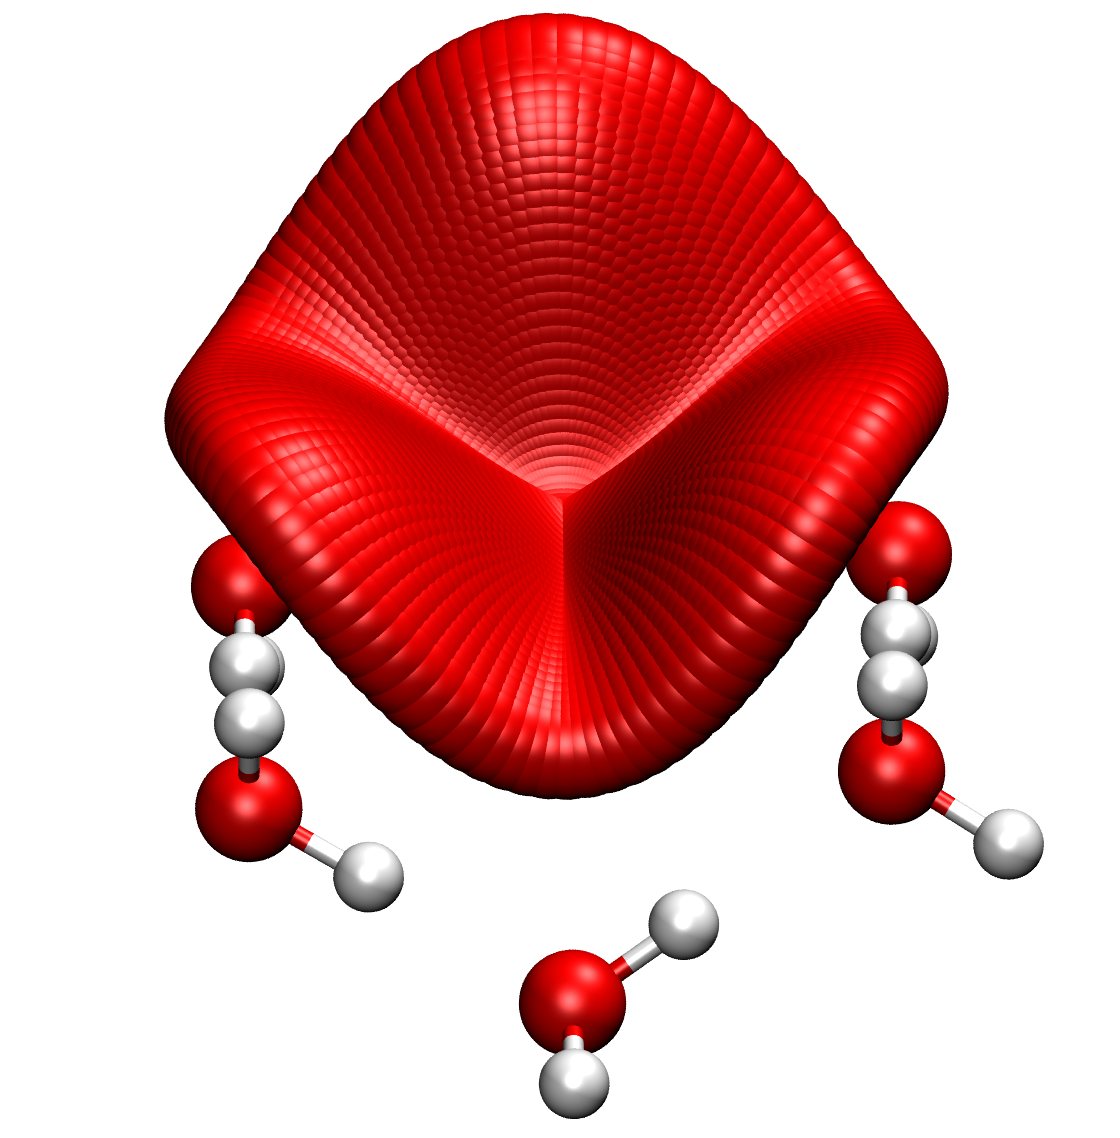
\includegraphics[width=.24\textwidth]{./img/SiteSnapshotMany.png}
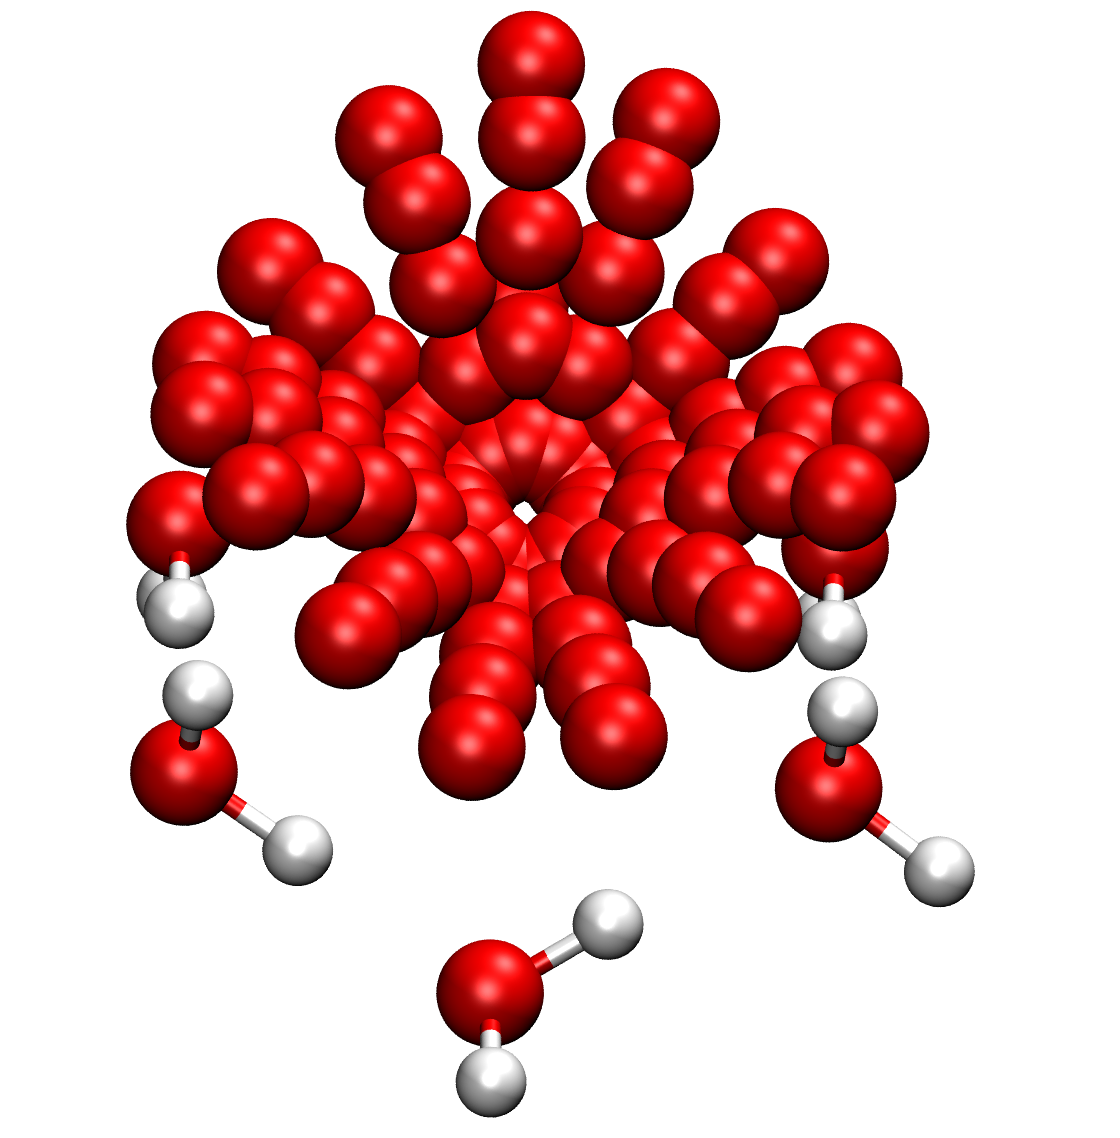
\includegraphics[width=.24\textwidth]{./img/SiteSnapshotOriginal.png}
\caption{The initial guesses for binding sites. The left is a visualization of the function
used, the right is the actual sites used as initial geometry. The molecules
below are the central ring.}
\label{Fig:Adv:BindingSitesGuess}
\end{figure}

We used the $\bhlyp$ functional with a $\zpe$ correction free adsorption energy 
of $-7.85~\kmo$, which is the weakest bound energy. For this energy,
there is reason to assume that there could be a more attractive binding site
somewhere in the central ring. To arrive at different binding sites, we used
a function to create initial data on the ring. Let the center of mass of the oxygen
atoms of the central ring be located at the origin $(0,0,0)^{\intercal}$ and let $y$ be
normal to the Fletcher surface. We can transform $(x,z)$ in polar coordinates with
$x=r \cos \phi$, $z=r \sin\phi$, $0 \leq r \leq \rmax$, $0 \leq \phi<2\pi$. The direction of the
unit vector $\bo e_x$ (that is $\bo e_r$ for $\phi=0$) and the value of $r_{\te{max}}$ are
chosen to ensure that there is an oxygen atom at the $xyz$ position
vector \mbox{$(\rmax,y < 0,0)^{\intercal}$}. In Figure
\ref{Fig:Adv:BindingSitesGuess}, the vector could be pointing towards the oxygen
%% CHECK: Kann man auch genauer bestimmen.
atom in the front. We found $\rmax=2.4~\Ang$.

In this coordinate system, we used the initial position
\begin{equation}
 y(r,\phi)=y_0+\rb{\vphantom{\frac 1 2}  A-B\cos\rb{3\phi}} \sin^2\rb{\frac{r}{\rmax}\frac\pi 2 }.
 \label{Adv:InitPos}
\end{equation}
This initial guess is
just to avoid unphysical starting positions with too far-off or too close $\tripo$
atoms. To that end, the parameters $y_0$, $A$ and $B$ are included, which we chose to be
$y_0=1.5~\Ang$, $A=1.5~\Ang$, $B=0.8~\Ang$.

We covered the area $(r,\phi) \in [0,\rmax] \times [0, 2\pi)$ with aequidistantly
distributed points according to $r_k=\rmin+k(\rmax-\rmin)/(N-1)$ and $\phi_l=2\pi l/M$,
$0 \leq k < N$ and $0 \leq l < M$, with $\rmin=0.4~\Ang$ and point numbers
$N=5$, $M=15$, leading to a total of 75 initial geometries. The aequidistant
distribution is chosen to cover as many local minima on the $x$-$z$ plane as
possible.

The oxygen atoms are added to the optimum geometry of the bare surface, where
the central ring is nearly undistorted.

\begin{figure}[b!]
%\hskip-2cm
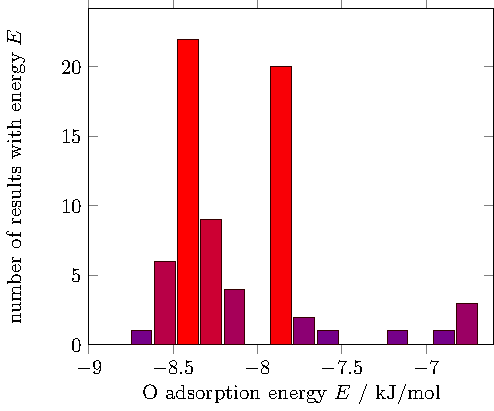
\includegraphics[width=.49\textwidth]{./TikzPics/TikzCreation/BindingEnergyDistribution/BindingEnergyDistribution.pdf}
\caption{Population of optimum geometry energies. Of the 75 initial guesses
according to \eqref{Adv:InitPos}, 71 converged to a minimum. One
geometry at $E=-5.01~\kmo$ is not included. Energies in $\kmo$.}
\label{Fig:Adv:BindingSitesEnergies}
\end{figure}

We then used the $\dlfind$ algorithm to find new energy minima. Of the 75
initial guesses, four did not converge in the six day computation time limit
of the JUSTUS cluster. The remaining initial positions were optimized
and yielded the energies plotted in Figure \ref{Fig:Adv:BindingSitesEnergies}.
One can see that most prominently, two adsorption energy values are found. One
around $-8.4~\kmo$ and one around $-7.85~\kmo$. In our first study, we only
found the less attractive geometry, which is directly above the center of mass
at $(0,2,0)^\intercal$, so close to the initial guess there. Other minima are
usually above lines connecting oxygen atoms. The most attractive geometries
profit of hydrogen bonds. The worst case, with an energy value of only
$-5.01~\kmo$, has the adsorbate positioned on a broken H bond. This minimum is
probably not very stable, it is only assumed by a single computation, all
others have energies of at least $-6.70~\kmo$. The strongest adsorption of
$-8.64~\kmo$ is also reached by only a single calculation. Therefore, we
conclude that there are two attractive energy minima to which more
than half of the initial geometries are drawn.

We recommend a central binding site at $(0,1.97,0)^\intercal$. This is not the
strongest binding site, but all optimum geometry searches starting close to it
converged there, so we can infer that there is no other energy minimum close by.
At greater distance from the center, we recommend further binding sites above
hydrogen atoms pointing out of the surface at a distance of 2.17~\Ang to the
hydrogen atom.

% We recommend the binding site $(0,2,0)^\intercal$ despite it being not the most
% attractive. The reason for that choice is that all other binding sites are
% located more or less above the central ring. This means that for simulations,
% they are not clearly within one ring or the other.

This becomes interesting when we consider hopping of adsorbates. In
Figure \ref{Fig:Adv:BindingSitesGuess}, the optima with $E<-8~\kmo$ lie to the
left and right. But then, due to quantum tunneling or temperature-dependent
vibrations, an O atom located above the center of mass can hop into another
optimum at the boundary of the ring, we may call it a transmission optimum, and
continue hopping into other rings from there. This mechanism should be
favourable for hopping ratios, but then there should be a preferred direction
of hopping on a Fletcher surface.

This may be interesting to study. However, one has to bear in mind that the
Fletcher surface is only an idealization in a zero temperature limit. Even at
temperatures in the cold ISM, the hydrogen atoms must give up their order. To
what extent this happens could be crucial to further analysis.


\subsection{Transition State}
\label{Sec:Adv:Trans}
\newcommand\hoht{\mbox{\enmat{\ho+\htw}}}
%% CHECK: Theory entry

\begin{figure}[b!]
%\hskip-2cm
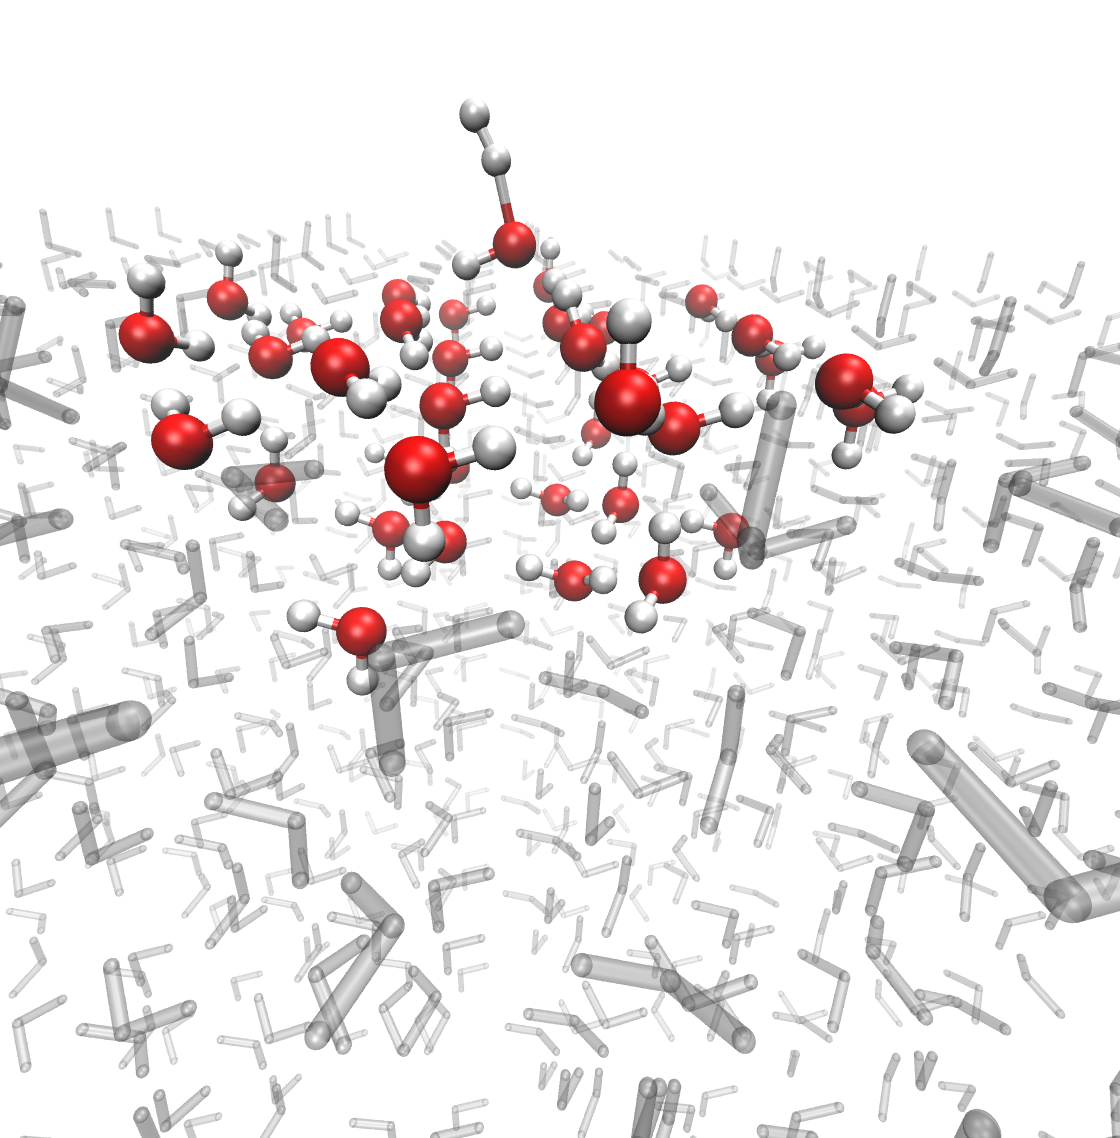
\includegraphics[width=.49\textwidth]{./img/FletcherAdsorption.png}
\caption{$\hoht$ transition state on Fletcher surface. Calculated with $\btlyp$.
Transparent atoms are in the MM region, red (O) an white (H) atoms in the QM
region.}
\label{Fig:Adv:TS}
\end{figure}

As mentioned before, transition states are important to reaction kinetics.
The energy difference between a system at the transition state and a system at
the optimum geometry yields the activation energy, a key ingredient to reaction
kinetics.

%% CHECK: Experimente? Zitate prüfen!
We studied the system $\hoht$, which is interesting for the reaction
\mbox{$\hoht\chemar\hto+\te H$}. This reaction is part of the water
formation scheme \cite{DishoeckHerbstNeufeld2013} and was studied
experimentally by Oba $\etal$\cite{ObaWatanabeHamaEtAl2012}.

We did not use any coupled-cluster references in this test but started
dircetly with DFT calculations. We used the $\btlyp$ functional because it was
closest to the average value for adsorption energies in the previous section.
We first calculated a gas-phase transition state using the dimer method (cf.
Section \ref{Sec:Theo:Minima}) and the $\tzvpd$ basis set. The transition
state geometry was placed on the relaxed Fletcher surface obtained with
$\btlyp$ and the hybrid $\tzvp/\tzvpd$ basis set. Unfortunately, the orientation
of the $\hoht$ subsystem on the surface is not clear. We assumed that the $\ho$
radical should be at least as close to the surface as the $\htw$ molecule, since
its adsorption energy is predicted to be far more attractive. We therefore
chose an initial geometry where the $\ho$ is placed above the center of the
central ring, the $\htw$ is slightly above it. To get a better guess for the
initial geometry, we then performed dimer method iteration with the smaller
$\svp$ basis set, despite it being not too good at describing geometries in the
benchmarks. Still, the dimer method typically requires more than one energy
evaluation per iteration cycle, which makes it computationally very expensive
for the hybrid basis set if the initial geometry is too far from the transition
state geometry. And indeed, it took $\svp$ 99 iteration cycles with a total of
405 energy and gradient evaluations to reach the transition state. The
subsequent optimization with the hybrid basis did, however, also require
87 iteration cycles with 477 energy and gradient evaluations. The RMSD between
the initial geometry and the $\svp$ transition state is $0.11~\Ang$
($0.91~\Ang$ for $\hoht$ alone) and the RMSD between the $\svp$
transition state and the hybrid basis transition state is $0.08~\Ang$
($0.22~\Ang$). As a comparison, the RMSD between the optimum geometry
(that is the energy minimum) and the transition state at the hybrid basis set
level is $0.06~\Ang$ ($0.90~\Ang$).

We can make some notes on the differences between our initial geometry and the
two transition states for different basis sets. The first one is that in this
case, $\svp$ seems to yield geometries that are reasonably close to the hybrid
basis geometry. That means that the geometries are not good
enough to consider the $\svp$ result a good approximation, but they are close
enough to serve as initial geometries. On the other hand, we can not be sure
whether the initial guess provided by $\svp$ is necessary at all, since the
majority of the convergence cycles occur at geometries that are already very
close to the transition state (when compared by RMSD value). This explains the
only slight difference in iteration cycles. The approach may still be sensible
for larger surface reactions. As a third note, the effect of orientation of the
adsorbate in the initial geometry may be an interesting topic for future
research.

\begin{figure}[t!]
%\hskip-2cm
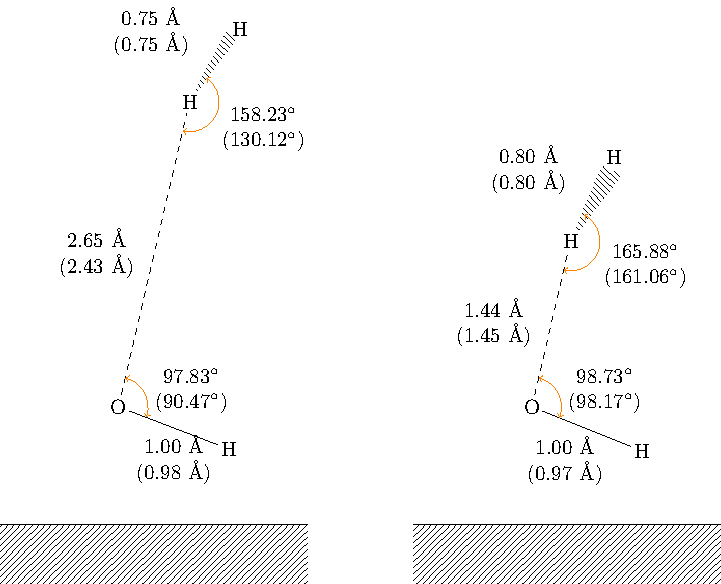
\includegraphics[width=.49\textwidth]{TikzPics/TikzCreation/HO.H2/HOH2.pdf}
\caption{Left: Optimum geometry for $\hoht$. Right: Transition state for $\hoht$.
Values are given for the adsorbate, values in parentheses are for the gas phase.
The
%% CHECK: Korrigiere fehlendes Surface-Optimum.
dihedral angles for the optimum geometry are 50.21$^{\circ}$ (33.58$^{\circ}$)
and for the transition state $2.58^{\circ}$ ($1.32^{\circ}$).}

\label{Fig:Adv:TSLengths}
\end{figure}


Relevant data for the bond distances and angles can be found in Figure
\ref{Fig:Adv:TSLengths} %, which does not give a good impression of
%surface deformation. 
Figure \ref{Fig:Adv:TS} shows the transition state
on the surface, where we have a better look at how the surface adjusts to
the adsorbate. Most notably, the H atoms pointing out of the surface are
tilted towards the O atom of $\ho$, while the H atom in $\ho$ is oriented
towards an $\hto$ molecule with a clipped hydrogen bond pointing out. The
$\htw$ molecule is too far from the surface to relevantly deform it.

Comparing gas-phase and adsorbate geometries for the transition state, we find
very good agreement. Both transition states are predicted nearly planar,
which is not true for the optimum geometry. Bond lengths do not change greatly
between transition state and optimum geometry, but the separation between the
two molecules decreases in the transition state. If we compare the gas-phase
geometry to the adsorbate geometry for the optimum, the disagreement is
stronger. The $\htw$ molecule has an increased separation from the $\ho$
radical. The ``upper'' H atom in $\htw$ tilts towards the surface. The stronger
deformation may be attributed to the fact that the interaction between $\ho$ and
$\htw$ is weaker in the optimum geometry and that therefore the surface affects
the optimum geometry stronger. 

\begin{figure}[t!]
%\hskip-2cm
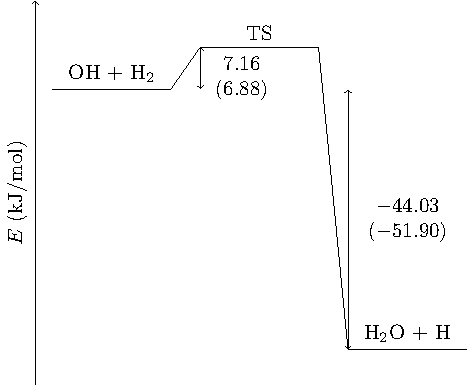
\includegraphics[width=.49\textwidth]{TikzPics/TikzCreation/HO.H2.Activation/HOH2Activation.pdf}
\caption{Energy diagram for the reaction $\ho + \htw \chemar \hto + \text H$ on
the surface. Values without parentheses use the $\zpering$ correction, values in
parentheses are uncorrected for ZPE.}
\label{Fig:Adv:ReactionEnergyDiagram}
\end{figure}
%% CHECK: Activation energy. Diagram with H2O+H?

A reaction energy diagram is presented in Figure
\ref{Fig:Adv:ReactionEnergyDiagram}. The influence of the
$\zpering$ correction is small for the transition state compared to the initial
$\ho + \htw$ energy, whereas the correction has a stronger effect on the prdocut
state, where it makes up $18\%$ of the energy.

We find the activation energy for the reaction \mbox{$\ho + \htw \chemar \hto +
\te H$} to be $7.16~\kmo$ and the reaction energy to be $-44.03~\kmo$. This does
not compare well to experimental data by Romanzin
\etal\cite{RomanzinIoppoloCuppenEtAl2011}, who found an activation energy of
$22.19~\kmo$ and a reaction energy of $-96.49~\kmo$. A source of error could be
the neglect of a finite temperature in the optimisation. Part of the problems
may also come from problems of DFT describing the breaking and rearrangement of
bonds of the given reactions, which we already encountered for gas-phase
reactions in Section \ref{Sec:Gas:Reaction}.


\section{Summary and Conclusion}
\label{Sec:Con}
We have designed a crystalline water $I_h$ Fletcher surface model for QM/MM
treatment. With this surface, we can give recommendations on the DFT functionals
that can be used in the QM part, which we base on an interaction energy
benchmark. The ZPE correction for the QM part was discussed and we compared
two different approaches, where we came to the conclusion that the
computationally less expensive $\zpering$ correction still provides results with
acceptable accuracy.

The adsorption energies calculated with the different functionals show not too
high disagreement among one another, however the ZPE corrected values yield
unphysical results for weakly adsorbed molecular species. We calculated average
values, which are the best recommendation we can give. The $\btlyp$ functional
is the functional closest to the average by MAD.

With the adsorption energies, we can calculate surface reaction eneriges of the
ER type based on gas-phase reaction energies at the $\ccsdtf/\vtz$ level of
%% CHECK: ccsdtf accuracy
theory. With the good results of the interaction energy benchmark and the
accuracy of $\ccsdtf$ for reaction energies, we can hope that the accuracy of
the surface reaction energies is good.

In two small investigations, we considered the
ability of the model to analyse different binding sites for a specific adsorbate
and the ability to describe transition states. We found two main classes of
binding sites for the $\tripo$ radical, and we found that the calculation of
transition states is computationally feasible.

Topics for further research could be the evaluation of orientation dependence
in both the adsorption of molecules and the calculation of transition states.
One could also look for a more systematic approach to analyse binding sites,
which may obtain a PES for some adsorbate.

Also, research in kinetic properties of surface reactions could be a next big
step. It can be hoped that insight into Langmuir-Hinshelwood type reactions can
be gained from the surface model, including diffusion rates for adsorbates as
well as surface reaction rates. One could also evaluate the influence of
tunneling on surface reactions and surface diffusion.

Since the crystalline surface is a rather strong idealisation, the model could
be further adjusted to include a grain surface. Such a model can describe
adsorption processes on ices only a few monolayers thick, thereby describing
early stages of water ice formation.

Additionally, less ordered surfaces are of interest to contemporary research. An
investigation of which of the results for the crystalline water $I_h$ surface
also apply to amorphous solid water and how strongly adsorption energies can
vary dependent on the surface composition should be interesting. The same goes
for incorporating impurities into the surface, most importantly CO$_2$.
Esepcially the accuracy of the $\zpering$ correction may greatly vary from surface type to
surface type, while additionally being not so well-defined for less symmetrical
surfaces.

In conclusion, the model established here is only a starting point for a
possibly wide range of theoretical research around the topic of interstellar
grain mantle composition and reactions. It seems appropriate to further advance
the application of \ep{ab initio} calculations in this field, which would help
both experimentalists and theoreticians to a better understanding of what
exactly is happening in interstellar clouds and possibly a more detailed
explanation of water formation in the interstellar medium within the next few
decades.

\section*{Acknowledgment}
I want to thank Professor J. Kästner for his support, Dr. Thanja Lamberts
for proofreading and Mr. Jan Meisner for his introduction to the topic, his
helpful suggestions and his company along the way.

%\clearpage
% \bibliographystyle{apalikenotitle}
\bibliographystyle{ieeetr}
%\bibliographystyle{plain}
%\bibliographystyle{abbr}

% \begin{thebibliography}
%\bibliography{MasterBib}
\bibliography{ShortTitles,MasterBib}{}
\end{document}